\chapter{Experiments and Research Results}
\label{chap:results}

\noindent\textbf{Reporting cutoff:} 16 September 2026.\\
\textbf{Purpose:} Advisor progress update, not a final performance claim.\\
\textbf{Analysis status:} Completed for the relogged artifacts. Root-cause
debugging was intentionally deferred.

\section{Relogged Campaign and Validity Audit}
\label{sec:results-validity}

The relogged campaign contains 66 estimator runs across seven featureless-floor
simulation datasets. Each condition was requested three times. The four dynamic
datasets contain baseline and nominal YOLO-filtered folders for both estimators
($4\times3\times4=48$ runs). The three static datasets contain baseline
ORB-SLAM3 and VINS-Fusion runs ($3\times3\times2=18$ runs). All directories
contain a trajectory, metadata, process-performance records, module records, and
a graceful-shutdown summary.

The validity audit distinguishes an operational estimator run from a valid
treatment comparison. All 66 runs initialized and produced usable log rows.
Two ORB-SLAM3 runs---\repo{dataset_static_nofloortexture_000/logging_20260916_02}
and \repo{logging_20260916_03}---have incomplete \repo{run_summary.csv} schemas:
their final inertial and map counters are absent. Their frame-level
\repo{performance.csv} records nevertheless reach \repo{imu_initialized=1},
\repo{inertial_ba1=1}, and \repo{inertial_ba2=1}, while
\repo{local_mapping.csv} records mapping activity. They are therefore retained
as operational runs; the missing summary fields are reported as a logging
anomaly rather than interpreted as estimator failure.

\begin{table}[htbp]
\centering
\caption{Relogged experiment progress and validity. ``Operational'' requires
graceful shutdown, estimator initialization, at least ten processed frames, and
a trajectory. Treatment validity additionally requires the intended filter to be
active and paired input counts and durations to differ by no more than 5\%.}
\label{tab:run-validity}
\small
\setlength{\tabcolsep}{4pt}
\begin{tabularx}{\textwidth}{>{\raggedright\arraybackslash}p{0.15\textwidth}rrrr>{\raggedright\arraybackslash}X}
\toprule
Run family & Attempted & Complete & Operational & Valid pairs & Interpretation \\
\midrule
Static baseline & 18 & 18 & 18 & -- & two incomplete ORB summaries \\
Dynamic baseline & 24 & 24 & 24 & -- & descriptive estimator logs \\
Dynamic ORB+YOLO & 12 & 12 & 12 & 1 of 12 & 11 input-mismatched pairs \\
Dynamic VINS+YOLO & 12 & 12 & 12 & 0 of 12 & filter inactive in every run \\
\midrule
Total & 66 & 66 & 66 & 1 treatment pair & preliminary campaign \\
\bottomrule
\end{tabularx}
\end{table}

Ground truth was extracted directly from each exact-name dataset rosbag's
\repo{/ground_truth/odometry} topic and associated with every repeat using source
header timestamps. Dataset association follows the containing folder name, not
the path recorded in \repo{run_metadata.csv}. The PC copies were used for
\repo{dataset_dynamic_nofloortexture_01_000} and
\repo{dataset_static_nofloortexture_001}; the other five bags were read from the
removable drive. That split was not a preference: both drive copies are
unreadable despite carrying complete metadata, as recorded in
\cref{tab:dataset-registry}. Each estimate is aligned to truth by a
rigid $SE(3)$ fit with scale fixed. Translational ATE RMSE and rotational geodesic
RMSE can therefore be reported. Relative pose error was added to the analysis
module after the cutoff and is reported in \cref{sec:rpe}; it required no
estimator re-runs.

The nominal VINS+YOLO treatment did not pass the mechanism check. Although its
metadata says \repo{filter=true}, all 12 runs report zero matched detection
frames, zero nonzero mask coverage, and zero removed dynamic tracks. These runs
remain useful for operational and compute inspection but cannot test semantic
filtering. ORB+YOLO recorded 9,706 matched and 10,764 missed detector frames over
20,470 mask-use rows, with no rejected masks. Its median mask coverage was zero
(IQR 0.0798), reflecting many frames without a used mask. Eleven of its 12
baseline/filter pairs differed in received image count by more than 5\%; only one
pair satisfies the predefined pairing rule. Consequently, no cross-treatment
accuracy conclusion is made.

\section{Non-Visual Baseline and Estimator Comparison}
\label{sec:results-proprio}

\subsection{Question, hypotheses, and conditions}

Until this experiment, every trajectory figure in this chapter reported visual
error against ground truth with nothing to compare it to, so a reader could see
how large the error was but not whether it was good. This section establishes the
dead-reckoning floor. The question is whether a non-visual estimator---wheel
odometry, IMU dead reckoning, or an EKF fusing them---provides usable
localization on the same recorded data, and whether the uncertainty each one
reports describes the error it actually makes.

Four hypotheses were registered before the metrics were computed:
\begin{itemize}
  \item[H1] Wheel-odometry drift is dominated by the measured yaw-rate scale
    error, so the two bags, whose scales err $+1.1\%$ and $-4.7\%$, should bow in
    opposite rotational directions.
  \item[H2] IMU-only dead reckoning diverges by orders of magnitude more than
    wheel odometry over the same interval.
  \item[H3] The EKF improves on both single-sensor estimators.
  \item[H4] All three report overconfident covariances, because a dead-reckoning
    noise model omits systematic scale error.
\end{itemize}

The independent variable is the estimator; everything else is held fixed within a
dataset. \Cref{tab:proprio-controls} records the controlled conditions. All five
estimators consume the same recordings and all visual runs replayed them under
identical settings.

The five datasets are not repeats of one condition. Only \repo{allsensor_000} and
\repo{allsensor_001} share a world. The remaining three vary two factors: object
placement, where \texttt{objonwallonly} restricts obstacles to the wall region and
clears the central floor, and floor texture, where \texttt{bayline} adds painted
bay lines to a surface that is otherwise featureless. No quantity is pooled across
worlds; each dataset is read as its own condition.

\begin{table}[htbp]
\centering
\caption{Controlled conditions for the estimator comparison. All five estimators
consume the same two recordings and are scored against the same ground truth over
the same interval.}
\label{tab:proprio-controls}
\small
\begin{tabularx}{\textwidth}{>{\raggedright\arraybackslash}p{0.26\textwidth}>{\raggedright\arraybackslash}X}
\toprule
Factor & Level \\
\midrule
Worlds & four: \repo{..._static_01_nofloortexture} (000, 001),
  \repo{..._static_nofloortexture_objonwallonly} (002),
  \repo{..._static_bayline_objonwallonly} (003),
  \repo{..._static_01_bayline} (004) \\
Floor & plain (000--002) versus bayline, i.e.\ painted lines (003, 004) \\
Scene dynamics & static \\
Floor & featureless \\
Datasets & five, \SIrange{81.8}{102.4}{\second} of simulated time and
  \SIrange{113.1}{142.3}{\metre} driven each \\
Dynamic filter & disabled in every run (\repo{filter=false}) \\
Replay rate & $0.5\times$ for both visual estimators \\
Ground truth & \repo{/ground_truth/odometry}, \SI{50}{\hertz}, header stamps \\
Alignment & rigid $SE(3)$, scale fixed, for cross-system comparison \\
Experimental unit, $n$ & one bag; $n=5$ across \emph{four} worlds. Only
  \texttt{static\_01} plain is repeated, and only twice \\
Visual configurations & VINS-Fusion; ORB-SLAM3 with loop closing enabled and
  disabled, one run each \\
\bottomrule
\end{tabularx}
\end{table}

\subsection{Validity}

All ten runs passed their predefined checks. The three baselines completed on
both bags with the planar assumption holding by a wide margin (maximum tilt
\SI{0.0018}{\degree} against a \SI{1}{\degree} threshold), the bicycle yaw-rate
model selected automatically on both, \repo{imu_orientation_used=NO} recorded in
every run, and the EKF applying 4\,355 and 4\,091 wheel corrections, matching the
wheel-odometry message counts exactly. Both VINS-Fusion runs processed every
image received (2\,639 and 2\,478), initialized once in \SI{0.33}{\second}, and
recorded no resets. Both ORB-SLAM3 runs shut down gracefully with no
tracking-loss events and inertial initialization at \SI{2.48}{\second} and
\SI{2.51}{\second}.

\begin{queried}[Queried]
ORB-SLAM3 receives fewer stereo pairs than are available on every dataset, while
VINS-Fusion receives all of them (2639, 2478 of 2479, 2628, 3102 and 3046). The
ORB shortfall is \SIrange{3.8}{11.9}{\percent} and varies by run as well as by
dataset: \SI{90.2}{\percent} and \SI{94.2}{\percent} of the available pairs on
\repo{allsensor_000} for the two configurations, \SI{96.2}{\percent} and
\SI{95.1}{\percent} on \repo{allsensor_003}. Its own counters report zero decode
failures, and the stereo timestamps are aligned to \SI{0}{\second} median offset
with \SI{100}{\percent} of pairs inside the \SI{20}{\milli\second} synchronisation
slop, so synchronisation is not what loses them.

The counter itself cannot say where they go: \repo{stereo_pairs_received} is
incremented inside the \emph{synchronised} callback, and the node keeps no count of
images arriving. What the source does show is an asymmetry in input buffering.
ORB-SLAM3 subscribes with \repo{rclcpp::SensorDataQoS()}, which is best-effort with
a depth of five, so a frame arriving while the tracking callback is busy is
discarded by the middleware and never recorded anywhere; VINS-Fusion subscribes
with \repo{KeepLast(100).reliable()} and buffers the same burst. \flag{The shortfall
is therefore most consistent with ORB-SLAM3 dropping frames at its own subscriber
under load, not with loss in transport.} The loop-closure-free runs support that
reading on three datasets, receiving more pairs than the enabled runs on
\repo{allsensor_000}, \repo{_001} and \repo{_002} while doing less work per frame,
though \repo{allsensor_003} runs the other way and the mechanism is not proven.
Trajectory accuracy over a shared interval is not obviously affected---ORB-SLAM3
is the more accurate of the two on some datasets despite the shortfall---but no
throughput, latency or per-frame compute comparison between the two estimators is
admissible until the loss is explained: the two estimators differ not only in
load but in input-queue policy, so such a comparison would measure the QoS choice
as much as the algorithm.
\end{queried}

\begin{queried}[Ruled out]
A plausible reading of these results is that the visual estimators lose to the EKF
because their input rate collapsed. The data does not support it. Source imagery
is regular at \SI{30.3}{\hertz} in simulated time on all five bags, with a median
inter-frame interval of \SI{0.0330}{\second} and no gap exceeding
\SI{0.1}{\second}; VINS-Fusion received and processed every frame on every
dataset, with zero skipped before the back end, and still trails the
cross-validated EKF on four of five. Frame loss is real for ORB-SLAM3 and remains
unexplained, but it cannot account for the margin, because the estimator with no
frame loss at all shows the same one.
\end{queried}

\begin{queried}[Queried]
ORB-SLAM3 was run in two configurations on every dataset, recorded as
\repo{logging_20260916_01} with loop closing enabled and
\repo{logging_20260916_02} with it disabled, and both are reported below as
separate systems. Within the enabled configuration the loop closer behaves very
differently per dataset (\cref{tab:orb-loop}), so those five trajectories are not
repeats of one condition and must not be pooled.

A counter reading \texttt{loop\_closures,0} does \emph{not} mean the loop closer
was inactive. On \repo{allsensor_000} it performed 447 place-recognition checks,
found 90 loop candidates and rejected all 90 on inertial geometry; on
\repo{allsensor_004} it found 114 and accepted none. The disabled runs are
distinguishable only in \repo{loop_closing.csv}, where every event carries
\texttt{current\_keyframe\_id}~$=-1$ and a duration below
\SI{0.003}{\milli\second}, the signature of a thread spinning with nothing queued
to it.
\end{queried}

\begin{table}[htbp]
\centering
\caption{Loop-closing activity in the enabled ORB-SLAM3 configuration
(\repo{logging_20260916_01}). Accepted closures are a small and dataset-dependent
fraction of candidates, and two datasets accept none at all despite the closer
running throughout. In the disabled configuration
(\repo{logging_20260916_02}) no keyframe ever reaches the loop closer on any
dataset.}
\label{tab:orb-loop}
\small
\begin{tabular}{lrrrr}
\toprule
Dataset & Place-recognition events & Candidates & Accepted & Global BA \\
\midrule
\repo{allsensor_000} & 537 & 90 & 0 & 0 \\
\repo{allsensor_001} & 379 & 2 & 2 & 2 \\
\repo{allsensor_002} & 274 & 11 & 1 & 1 \\
\repo{allsensor_003} & 591 & 64 & 1 & 0 \\
\repo{allsensor_004} & 713 & 114 & 0 & 0 \\
\bottomrule
\end{tabular}
\end{table}

\begin{queried}[Provenance gap]
\repo{run_metadata.csv} records 22 parameters and loop-closure state is not among
them, so the whole distinction rests on the directory name---and that name does
not mean the same thing everywhere in this chapter. In the relogged campaign of
\cref{sec:results-validity}, \repo{logging_20260916_01} through \repo{_03} are
three \emph{repeats} of one configuration, all with an active loop closer. In the
\repo{allsensor} campaign reported here, \repo{_01} and \repo{_02} are two
\emph{configurations}, loop closing enabled and disabled, with one run each. The
same suffix therefore encodes a repeat index in one section and an experimental
factor in the next. The metadata for the two bag-000 runs is identical apart from the experiment
identifier, output path and start time, and both name the same installed
configuration file, so nothing in the recorded provenance distinguishes an
enabled run from a disabled one. The distinction used in this chapter was
recovered from \repo{loop_closing.csv} after the fact. The logger should record
the loop-closing and global-BA switches explicitly before any further ORB-SLAM3
campaign.
\end{queried}

\subsection{Accuracy results}

\Cref{tab:proprio-accuracy} reports all five estimators. Aligned ATE is the only
column comparable across systems, because the visual estimators build their own
world frames while the baselines start from the ground-truth pose.

\begin{table}[htbp]
\centering
\caption{Estimator comparison on the five \repo{allsensor} bags, which span four
worlds and both floor conditions; they are not repeats of one another except for
\repo{allsensor_000} and \repo{allsensor_001}. Bold marks the best aligned ATE of
each dataset---the EKF on four of five, VINS-Fusion on \repo{allsensor_004}. ``Aligned ATE'' is
RMSE after a rigid $SE(3)$ fit with scale fixed, the convention used throughout
this chapter. ``Anchored'' columns are the direct difference from ground truth
with no alignment and are defined only for the estimators that start from the
ground-truth pose; the visual estimators' own world frames make that subtraction
meaningless, so those cells are set to --. Drift is the final position error as a
fraction of distance driven.}
\label{tab:proprio-accuracy}
\small
\setlength{\tabcolsep}{5pt}
\resizebox{\textwidth}{!}{%
\begin{tabular}{lllrrrrr}
\toprule
Dataset & World & Estimator & Aligned ATE & Anchored RMS & Anchored final &
  Drift & Final yaw \\
 & & & [\si{\metre}] & [\si{\metre}] & [\si{\metre}] & [\si{\percent}] &
  [\si{\degree}] \\
\midrule
\repo{allsensor_000} & \texttt{static\_01} & IMU dead reckoning & 21.697 & 39.353 &
  47.597 & 40.66 & $+2.19$ \\
 & plain & Wheel odometry & 2.801 & 4.732 & 4.767 & 4.07 & $-13.76$ \\
 & & VINS-Fusion & 0.616 & -- & -- & -- & -- \\
 & & ORB-SLAM3 & 0.579 & -- & -- & -- & -- \\
 & & ORB-SLAM3 (no LC) & 0.285 & -- & -- & -- & -- \\
 & & \textbf{EKF wheel+IMU} & \textbf{0.190} & 0.281 & 0.122 & \textbf{0.10} &
  $+0.19$ \\
\midrule
\repo{allsensor_001} & \texttt{static\_01} & IMU dead reckoning & 12.617 & 14.728 &
  23.741 & 20.99 & $+1.33$ \\
 & plain & Wheel odometry & 0.979 & 1.826 & 2.426 & 2.15 & $-12.95$ \\
 & & VINS-Fusion & 0.383 & -- & -- & -- & -- \\
 & & ORB-SLAM3 & 0.372 & -- & -- & -- & -- \\
 & & ORB-SLAM3 (no LC) & 0.516 & -- & -- & -- & -- \\
 & & \textbf{EKF wheel+IMU} & \textbf{0.308} & 0.351 & 0.303 & \textbf{0.27} &
  $+0.11$ \\
\midrule
\repo{allsensor_002} & \texttt{objonwallonly} & IMU dead reckoning & 13.237 &
  16.359 & 17.728 & 15.39 & $+1.36$ \\
 & plain & Wheel odometry & 1.485 & 2.888 & 4.332 & 3.76 & \flag{$-30.11$} \\
 & & VINS-Fusion & 0.558 & -- & -- & -- & -- \\
 & & ORB-SLAM3 & 0.602 & -- & -- & -- & -- \\
 & & ORB-SLAM3 (no LC) & 1.796 & -- & -- & -- & -- \\
 & & \textbf{EKF wheel+IMU} & \textbf{0.256} & 0.345 & 0.346 & \textbf{0.30} &
  $-0.68$ \\
\midrule
\repo{allsensor_003} & \texttt{bayline\_} & IMU dead reckoning & 45.562 & 62.903 &
  74.745 & \flag{53.16} & $-5.84$ \\
 & \texttt{objonwallonly} & Wheel odometry & 3.192 & 3.979 & 9.231 & 6.57 &
  \flag{$-37.17$} \\
 & bayline & VINS-Fusion & 0.784 & -- & -- & -- & -- \\
 & & ORB-SLAM3 & \flag{6.481} & -- & -- & -- & -- \\
 & & ORB-SLAM3 (no LC) & 0.515 & -- & -- & -- & -- \\
 & & \textbf{EKF wheel+IMU} & \textbf{0.423} & 0.668 & 1.240 & \textbf{0.88} &
  $-7.20$ \\
\midrule
\repo{allsensor_004} & \texttt{static\_01\_} & IMU dead reckoning & 26.709 & 41.476 &
  48.099 & 33.81 & $-1.35$ \\
 & \texttt{bayline} & Wheel odometry & 3.241 & 5.124 & 5.791 & 4.07 & $-17.68$ \\
 & bayline & \textbf{VINS-Fusion} & \textbf{0.425} & -- & -- & -- & -- \\
 & & ORB-SLAM3 & 1.237 & -- & -- & -- & -- \\
 & & ORB-SLAM3 (no LC) & 0.905 & -- & -- & -- & -- \\
 & & EKF wheel+IMU & 0.494 & 0.776 & 0.831 & 0.58 & $-5.30$ \\
\bottomrule
\end{tabular}}
\end{table}

H2 and H3 are supported on every dataset. IMU-only dead reckoning is 7.7 to 14.3
times worse than wheel odometry, and the EKF improves on both single sensors by an order
of magnitude everywhere.

H3's stronger form---that the EKF also beats the visual estimators---holds on four
of the five datasets but not universally, and the margin is much narrower than the
three-dataset version of this section reported. \flag{That earlier figure of
``3.0, 1.2 and 2.2 times'' was computed against ORB-SLAM3 with loop closing
enabled, which is not the best visual result available.} Measured against the best
visual estimator of each dataset, and using the cross-validated EKF so that no
in-sample tuning advantage is carried
(\cref{tab:proprio-xval}), the margins are 1.38, 1.41, 2.53, 1.31 and
\num{1.13}. On \repo{allsensor_004} the in-sample EKF at \SI{0.494}{\metre} is
beaten outright by VINS-Fusion at \SI{0.425}{\metre}; only the cross-validated
figure of \SI{0.377}{\metre} is ahead. The honest statement is that a
five-state proprioceptive filter is competitive with, and usually better than,
stereo visual-inertial SLAM in these scenes---not that it dominates it.

Two expectations about scene content are not supported. Clearing the central floor
did not penalise vision: the visual errors on \repo{allsensor_002} (0.558 and
\SI{0.602}{\metre}) sit close to \repo{allsensor_000} (0.616 and
\SI{0.579}{\metre}). \flag{Nor did adding the bay markings help it}---the two
\texttt{bayline} datasets give VINS-Fusion 0.784 and \SI{0.425}{\metre} against
0.616, 0.383 and \SI{0.558}{\metre} on the plain floors, which is no improvement.
That null result is weaker evidence than the factor's name implies: both floor
conditions rest on the same flat, untextured base and differ only by fourteen
painted bay outlines covering a small fraction of the floor
(\cref{fig:floor-treatments}), so what was varied is bay markings, not surface
texture.
What the textured datasets did change is the \emph{proprioceptive} side: both
carry the largest wheel yaw-rate scale errors of the five, and both degrade the
EKF accordingly (\cref{sec:h1-falsified}).

The mechanism is visible in the last two columns and is the substantive finding
of this section: \emph{the two proprioceptive sensors fail in complementary ways}.
The IMU holds heading to \SI{2.19}{\degree} and \SI{1.33}{\degree} while losing
position catastrophically; the wheels hold position to a few percent while losing
\SI{13}{\degree} of heading. The EKF is better than either in \emph{both}
quantities simultaneously, reaching \SI{0.19}{\degree} of final heading error---an
order of magnitude better than the gyroscope alone---because the wheel yaw rate is
used to observe the gyroscope bias rather than heading, so the filter never
inherits the wheels' own heading drift (\cref{sec:proprio-method}).

\begin{figure}[htbp]
  \centering
  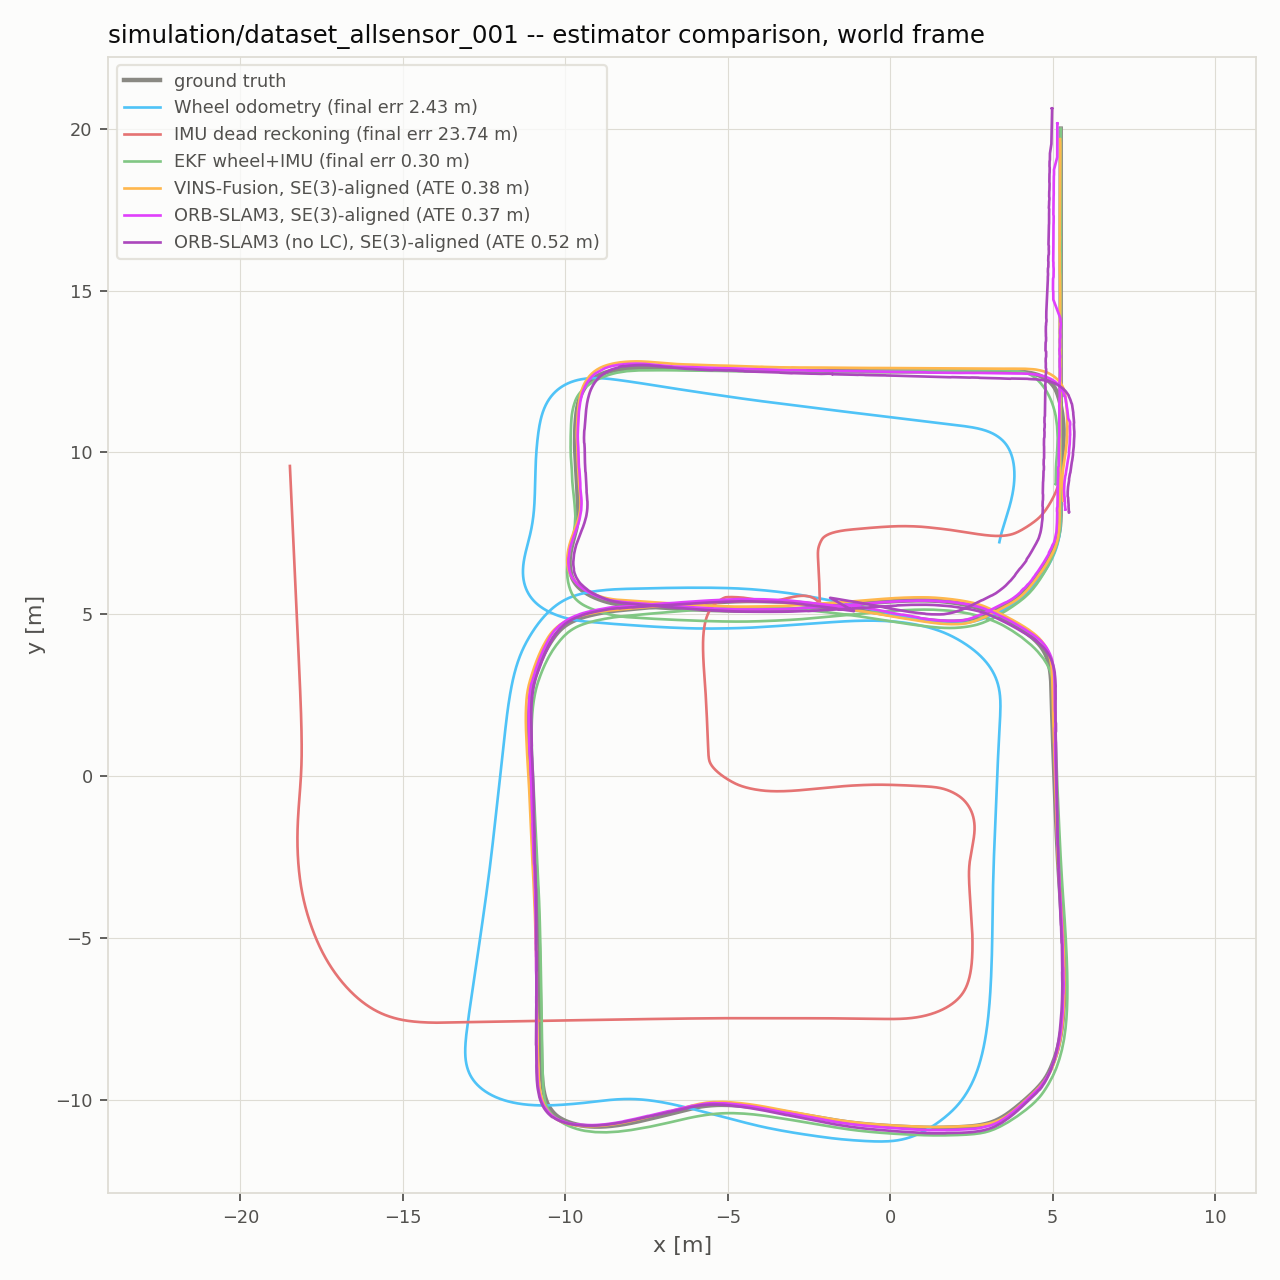
\includegraphics[width=0.82\textwidth]{../../../output/compare/simulation/exp-estimator-baseline/proprio_trajectories_dataset_allsensor_001_light.png}
  \caption{Estimator comparison on \repo{dataset_allsensor_001}, world frame. The
  baselines are drawn as estimated; the visual estimators are drawn after the same
  rigid $SE(3)$ alignment used for their metrics, because their own world frames
  are arbitrary. Ground truth is hidden beneath the EKF, VINS and ORB traces for
  most of the run. Wheel odometry (blue) bows consistently outward; IMU dead
  reckoning (red) leaves the building.}
  \label{fig:proprio-trajectories}
\end{figure}

\subsection{Falsification of H1, and the drift mechanism}
\label{sec:h1-falsified}

H1 is \flag{falsified} across all five datasets. If drift followed the fitted
yaw-rate scale, the bag with the most nearly correct scale would drift least. The
opposite holds (\cref{tab:h1}): \repo{allsensor_002} has the best scale of the
five, $+0.34\%$, and \SI{-30.11}{\degree} of heading error, while
\repo{allsensor_004} has the worst scale, $-7.50\%$, and only
\SI{-17.68}{\degree}. All five heading errors share a sign; the scale errors do
not.

\begin{table}[htbp]
\centering
\caption{Wheel-odometry heading drift against the fitted yaw-rate scale.
``Rotation'' is the total unsigned ground-truth rotation of the run, and
``error/rotation'' expresses the final heading error as a fraction of it. Scale
error and heading error correspond in neither sign nor magnitude. The last column
is the constant-offset prediction described below: the mean yaw-rate residual of
the run multiplied by its duration, which matches the measured error to within
\SI{1.4}{\degree} on every dataset, and to within \SI{0.5}{\degree} on three of
five.}
\label{tab:h1}
\small
\resizebox{\textwidth}{!}{%
\begin{tabular}{lrrrrr}
\toprule
Dataset & Yaw-rate scale & Final yaw error & Rotation & Error/rotation &
  Offset prediction \\
 & [\si{\percent}] & [\si{\degree}] & [\si{\degree}] & [\si{\percent}] &
  [\si{\degree}] \\
\midrule
\repo{allsensor_000} & $+1.10$ & $-13.76$ & 536 & $-2.566$ & $-13.81$ \\
\repo{allsensor_001} & $-4.73$ & $-12.95$ & 852 & $-1.519$ & $-13.37$ \\
\repo{allsensor_002} & $+0.34$ & \flag{$-30.11$} & 865 & $-3.481$ & $-31.03$ \\
\repo{allsensor_003} & $-6.25$ & \flag{$-37.17$} & 1123 & $-3.309$ & $-38.51$ \\
\repo{allsensor_004} & $-7.50$ & $-17.68$ & 895 & $-1.976$ & $-18.03$ \\
\bottomrule
\end{tabular}}
\end{table}

The proximate mechanism is nevertheless now identified, and it is simpler than a
scale error. The wheel model's yaw rate carries a small persistent \emph{offset}
against ground truth, averaged over all moving samples: \SI{-0.00277}{},
\SI{-0.00285}{} and \SI{-0.00624}{\radian\per\second} on the three bags. Because
heading is the time integral of that rate, an offset produces an error that grows
linearly with elapsed time rather than with rotation. Multiplying each offset by
its run duration reproduces the measured error to within \SI{1.4}{\degree} on all
five datasets (\cref{tab:h1}, last column), including the two textured-floor runs
that were recorded after the mechanism was proposed. The drift is accounted for.

\begin{queried}[Corrected]
An earlier reading of this experiment proposed that the offset came from the
bicycle model averaging the two kingpin angles, since $\tan$ of a mean is not the
mean of $\tan$. That explanation is \emph{wrong} and is withdrawn. Recomputing the
yaw rate as the mean of each wheel's own bicycle-equivalent rate changes the
residual from \SI{-0.00277}{} to \SI{-0.00288}{}, from \SI{-0.00285}{} to
\SI{-0.00296}{}, and from \SI{-0.00624}{} to \SI{-0.00630}{\radian\per\second}---
under \SI{4}{\percent} in every case, two orders of magnitude short of what the
observed drift requires. The averaging is not the source.
\end{queried}

What remains open is the origin of the offset itself. It is not a pure magnitude
error: splitting the residual by turn direction gives $+0.0109$ against $-0.0142$
on \repo{allsensor_000} and $+0.0075$ against
$-0.0292$~\si{\radian\per\second} on \repo{allsensor_002}, so the model
under-rotates in both directions \emph{and} carries a directional bias on top. On
\repo{allsensor_001}, whose route returns to its starting heading, both directions
are negative and only the bias is visible. A steering-angle zero offset, an
unmodelled slip angle, and a kingpin-geometry error are all consistent with what
has been measured so far and none has been tested.

This matters beyond wheel odometry, and the two textured-floor datasets turn what
was a caveat into a measurement. The EKF observes its gyroscope bias through
exactly this wheel yaw rate (\cref{sec:proprio-method}), so a persistent offset in
the wheel rate is absorbed into the estimated bias and reappears as heading error.
\Cref{tab:ekf-coupling} shows the two tracking each other across the five
datasets: where the wheel yaw-rate scale is within \SI{1.1}{\percent} of unity the
EKF holds heading to \SI{0.42}{\degree} or better, and where it is \SI{6}{} to
\SI{7.5}{\percent} low the EKF's heading error rises roughly tenfold.

\begin{table}[htbp]
\centering
\caption{The EKF's heading error follows the quality of the wheel yaw rate it uses
to observe its gyroscope bias. The filter is no better than its rate reference,
which is the cost of making the bias observable at all.}
\label{tab:ekf-coupling}
\small
\resizebox{\textwidth}{!}{%
\begin{tabular}{llrrrr}
\toprule
Dataset & Floor & Wheel yaw scale & Wheel yaw $\sigma$ & EKF yaw RMS & EKF ATE \\
 & & & [\si{\radian\per\second}] & [\si{\degree}] & [\si{\metre}] \\
\midrule
\repo{allsensor_000} & plain & 1.0110 & 0.0659 & 0.35 & 0.190 \\
\repo{allsensor_002} & plain & 1.0034 & 0.0705 & 0.30 & 0.256 \\
\repo{allsensor_001} & plain & 0.9527 & 0.0804 & 0.42 & 0.308 \\
\repo{allsensor_003} & bayline & 0.9375 & 0.1192 & \flag{3.54} & 0.423 \\
\repo{allsensor_004} & bayline & 0.9250 & 0.0613 & \flag{3.41} & 0.494 \\
\bottomrule
\end{tabular}}
\end{table}

An earlier version of this section, written when only the three plain-floor
datasets existed, recorded that the EKF held heading below \SI{0.7}{\degree}
everywhere and inferred that the absorbed error was small. \flag{That inference
does not survive the textured-floor datasets} and is withdrawn: the coupling is
the dominant term in the EKF's heading error whenever the wheel rate is poor, and
it sets a floor on the filter's accuracy that no amount of gyroscope quality can
lift.

One prediction of the original reasoning did survive, and is visible in
\cref{fig:proprio-covariance}: wheel-odometry error stays flat at roughly
\SI{6}{\milli\metre} for the first \SI{9.5}{\second}, the initial straight run,
and only grows once the first turn begins. Turning, not distance, starts the
error; the offset then sustains it.

\subsection{Covariance consistency}

H4 is supported emphatically. \Cref{tab:proprio-covariance} reports the average
normalised estimation error squared,
$\mathrm{NEES}=\mathbf{e}^{\top}\mathbf{P}^{-1}\mathbf{e}$ with
$\mathbf{e}=[\Delta x,\Delta y,\Delta\theta]$, which a correctly scaled covariance
makes average 3.0, together with the fraction of the run for which the truth lies
inside the reported $k\sigma$ bounds.

\begin{table}[htbp]
\centering
\caption{Covariance consistency of the non-visual estimators. A consistent filter
gives $\mathrm{ANEES}=3.0$ and $\sigma$-coverages of 0.683, 0.954 and 0.997. Every
estimator is overconfident by roughly two orders of magnitude. Neither VINS-Fusion
nor ORB-SLAM3 writes a pose covariance, so neither can be tested here.}
\label{tab:proprio-covariance}
\small
\begin{tabular}{llrrrrl}
\toprule
Dataset & Estimator & ANEES & $1\sigma$ & $2\sigma$ & $3\sigma$ & Verdict \\
\midrule
\repo{allsensor_000} & Wheel odometry & 569.4 & 0.309 & 0.390 & 0.408 & overconfident \\
 & IMU dead reckoning & 311.0 & 0.005 & 0.022 & \flag{0.043} & overconfident \\
 & EKF wheel+IMU & 64.7 & 0.426 & 0.767 & 0.879 & overconfident \\
\midrule
\repo{allsensor_001} & Wheel odometry & 263.9 & 0.015 & 0.131 & 0.187 & overconfident \\
 & IMU dead reckoning & 339.9 & 0.001 & 0.009 & \flag{0.021} & overconfident \\
 & EKF wheel+IMU & 123.2 & 0.194 & 0.439 & 0.537 & overconfident \\
\midrule
\repo{allsensor_002} & Wheel odometry & 729.4 & 0.140 & 0.143 & 0.145 & overconfident \\
 & IMU dead reckoning & 244.7 & 0.017 & 0.045 & \flag{0.147} & overconfident \\
 & EKF wheel+IMU & 114.5 & 0.193 & 0.350 & 0.501 & overconfident \\
\midrule
\repo{allsensor_003} & Wheel odometry & 406.7 & 0.260 & 0.343 & 0.459 & overconfident \\
 & IMU dead reckoning & \flag{1504.3} & 0.010 & 0.018 & \flag{0.035} & overconfident \\
 & EKF wheel+IMU & 79.1 & 0.034 & 0.291 & 0.476 & overconfident \\
\midrule
\repo{allsensor_004} & Wheel odometry & 785.0 & 0.154 & 0.157 & 0.162 & overconfident \\
 & IMU dead reckoning & 289.5 & 0.004 & 0.017 & \flag{0.044} & overconfident \\
 & EKF wheel+IMU & 78.6 & 0.254 & 0.330 & 0.570 & overconfident \\
\midrule
\multicolumn{2}{l}{\emph{consistent reference}} & 3.0 & 0.683 & 0.954 & 0.997 & -- \\
\bottomrule
\end{tabular}
\end{table}

The IMU case is the starkest: its $3\sigma$ envelope contains the truth for
between \SI{2.1}{\percent} and \SI{14.7}{\percent} of each run, and its worst
ANEES, 1504 on \repo{allsensor_003}, is the largest figure in the experiment.
A consumer weighting this estimate by its stated covariance---a costmap, a
pose-graph edge, a relocaliser gate---would trust it tens of times more than it
deserves. Wheel odometry on \repo{allsensor_002} is the single worst case in the
experiment, ANEES 785 on \repo{allsensor_004} with $3\sigma$ coverage of 0.162, which is
consistent with
the heading offset of \cref{sec:h1-falsified}: the covariance model contains no
term for a persistent rate bias, so the larger that bias, the further the claimed
uncertainty falls behind the real error. The EKF is the least bad on every
dataset, at $3\sigma$ coverage between 0.476 and 0.879, and
\cref{fig:proprio-covariance} shows why: its NEES is genuinely near 3 during the
opening straight and only departs once turning begins, which is the same moment
the unmodelled heading error appears.

\begin{figure}[htbp]
  \centering
  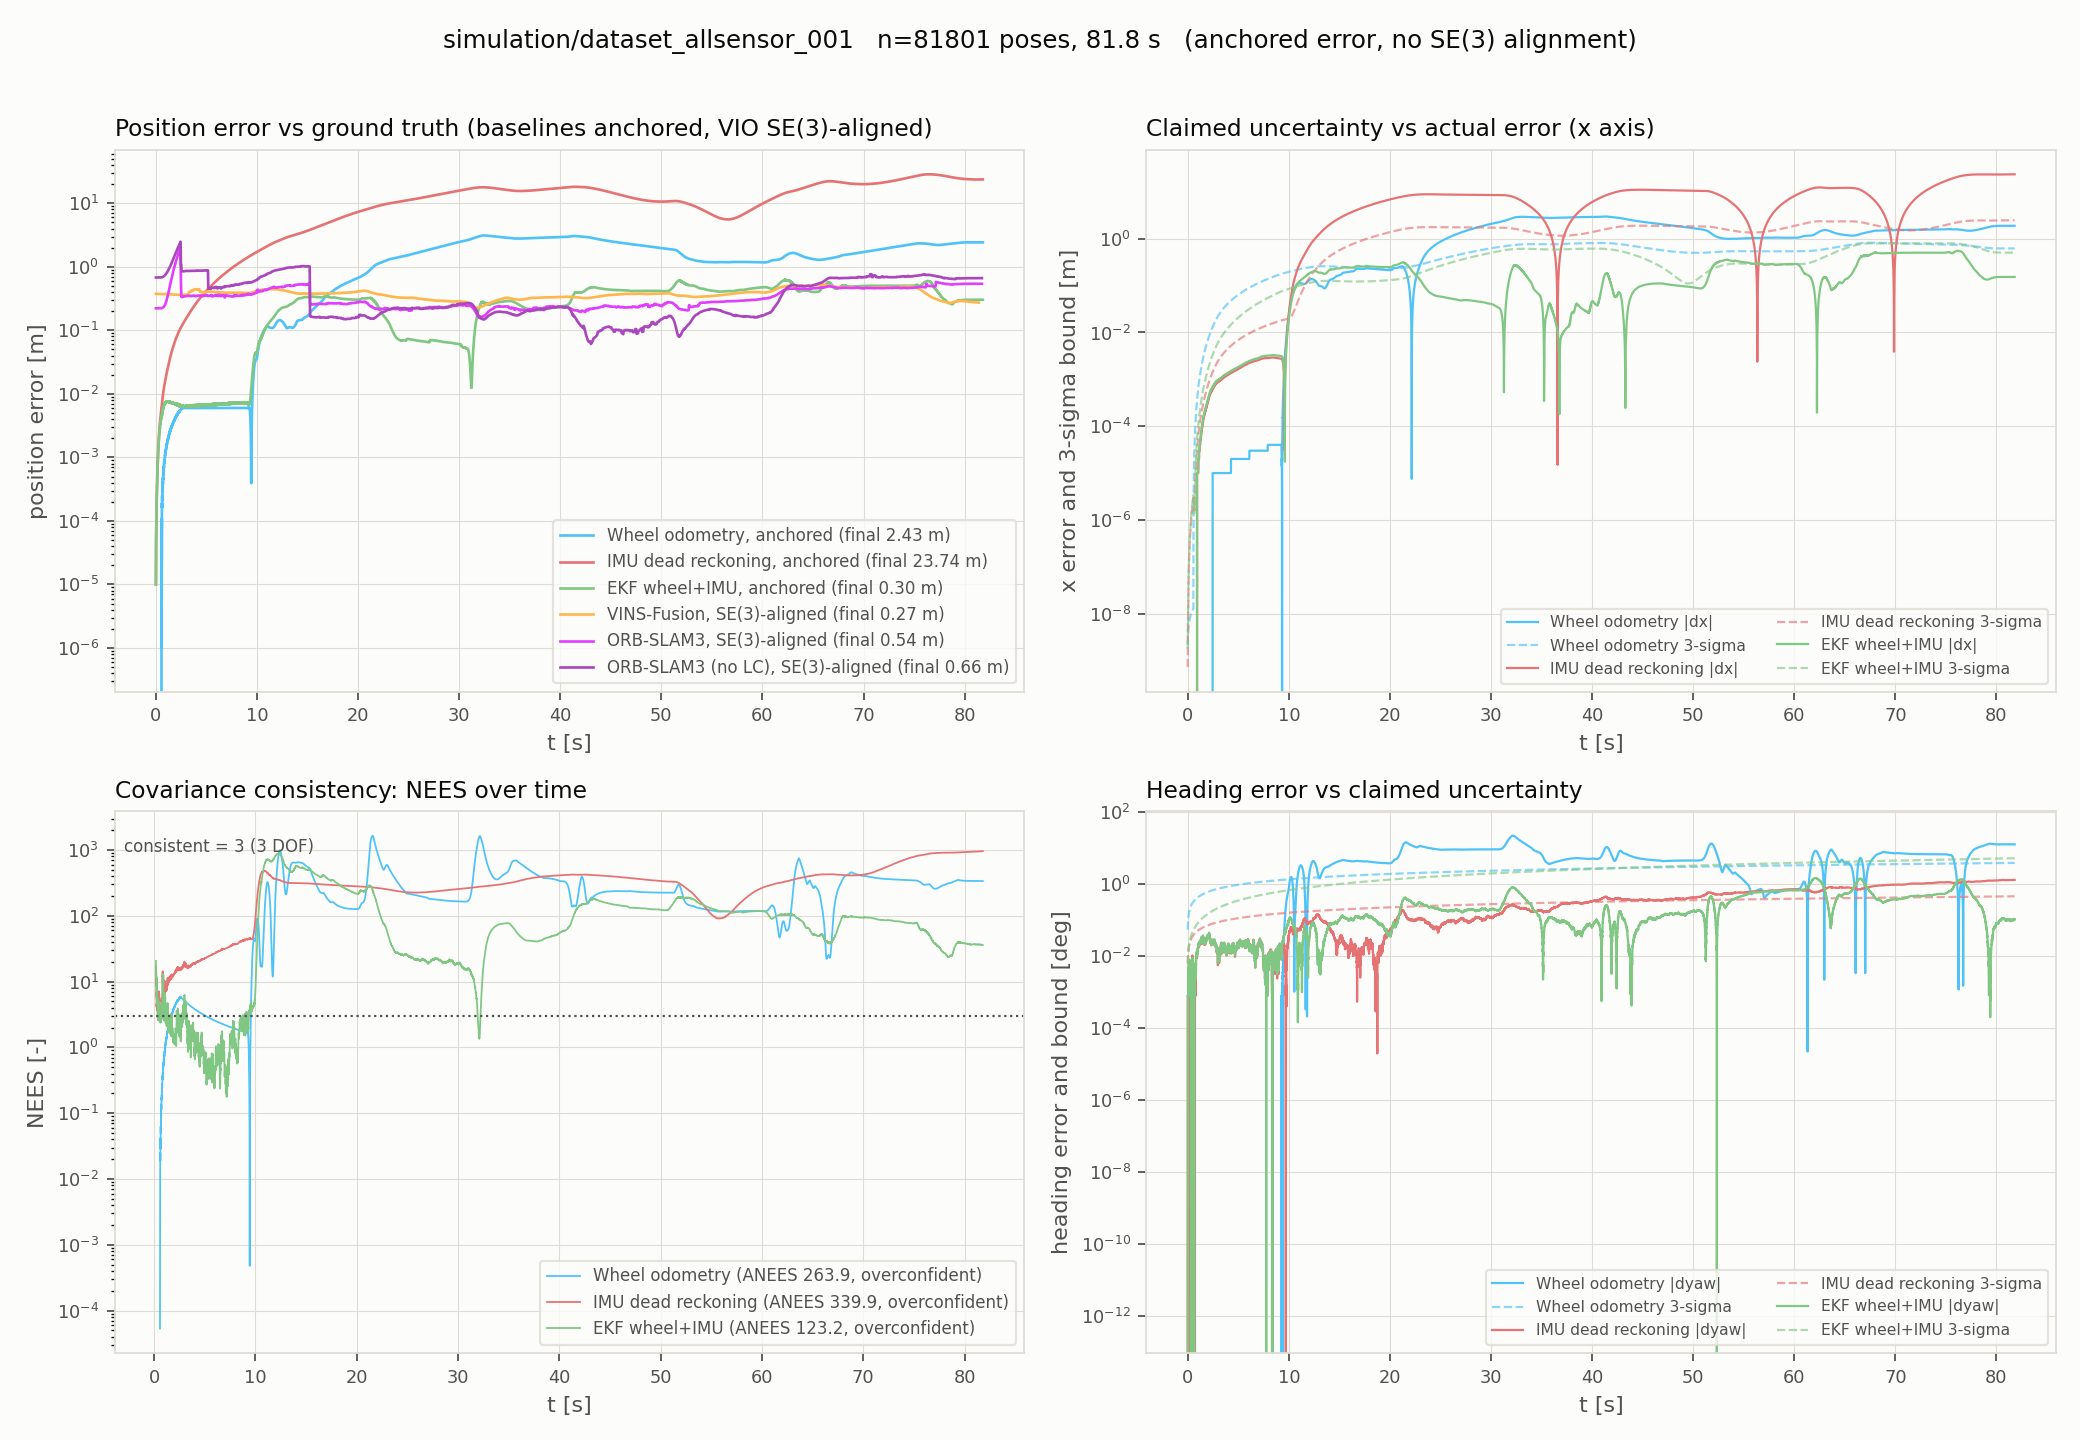
\includegraphics[width=\textwidth]{../../../output/compare/simulation/exp-estimator-baseline/proprio_covariance_dataset_allsensor_001_light.png}
  \caption{Error against claimed uncertainty for \repo{dataset_allsensor_001}.
  Top left: position error over time, baselines anchored and visual estimators
  $SE(3)$-aligned. Top right and bottom right: absolute error against the
  estimator's own $3\sigma$ bound, in $x$ and in heading; where the solid line
  sits above the dashed line of the same colour the filter is overconfident.
  Bottom left: NEES against the consistent value of 3. The step near
  \SI{9.5}{\second} in every panel is the first turn of the run.}
  \label{fig:proprio-covariance}
\end{figure}

\begin{queried}[Method caveat]
The $\chi^2$ interval behind the verdict column assumes independent samples. At
\SI{200}{\hertz} consecutive dead-reckoning errors are almost perfectly
correlated, so the test is run on a \SI{1}{\hertz} subsample (81 to 102 samples per dataset).
That reduces the dependence but does not remove it, and the verdicts should be
read as indicative. The $\sigma$-coverage columns make no independence assumption
and are the sturdier statement.
\end{queried}

\subsection{Cross-validation of the EKF noise model}

The EKF's noise model is derived from the same recording it runs on, whereas the
visual estimators receive no comparable tuning. The wheel and IMU baselines are
unaffected---their measured $\sigma$ values enter only the covariance, never the
trajectory---but the EKF's values enter the Kalman gain and so do change its
output. The comparison was therefore repeated with the noise models exchanged
between bags (\cref{tab:proprio-xval}).

\begin{table}[htbp]
\centering
\caption{EKF accuracy with an in-sample and an out-of-sample noise model. The
change is negative on four of five bags---the borrowed model is \emph{better}
there---and the mean change is about $-10\%$, which is the signature of no
systematic in-sample advantage.}
\label{tab:proprio-xval}
\small
\begin{tabular}{llrr}
\toprule
Dataset & Noise model from & Aligned ATE [\si{\metre}] & Change \\
\midrule
\repo{allsensor_000} & same bag & 0.190 & -- \\
 & \repo{allsensor_001} & 0.206 & $+8.8\%$ \\
\midrule
\repo{allsensor_001} & same bag & 0.308 & -- \\
 & \repo{allsensor_000} & 0.263 & $-14.5\%$ \\
\midrule
\repo{allsensor_002} & same bag & 0.256 & -- \\
 & \repo{allsensor_000} & 0.220 & $-13.9\%$ \\
\midrule
\repo{allsensor_003} & same bag & 0.423 & -- \\
 & \repo{allsensor_000} & 0.392 & $-7.1\%$ \\
\midrule
\repo{allsensor_004} & same bag & 0.494 & -- \\
 & \repo{allsensor_000} & 0.377 & $-23.8\%$ \\
\bottomrule
\end{tabular}
\end{table}

The noise model transfers between runs, and on four of the five bags the borrowed
model is the better one, which no in-sample advantage could produce. The EKF's
accuracy is therefore a property of the estimator rather than of having seen the
answer. Cross-validated it reaches 0.206, 0.263, 0.220, 0.392 and
\SI{0.377}{\metre}, which is 1.38, 1.41, 2.53, 1.31 and 1.13 times better than the
best visual estimator of each dataset. Notably the cross-validated figure on
\repo{allsensor_004} recovers a lead that the in-sample filter did not have.

\subsection{Interpretation and limitations}

Within these two recordings, a five-state planar filter over wheel encoders and a
gyroscope localises more accurately than either stereo visual-inertial system.
That is an uncomfortable result for the thesis premise and is reported as
measured. It does not show that vision is unnecessary; it shows that in this
condition vision has not yet earned its compute, and that the justification has to
come from capabilities dead reckoning does not have at all---loop closure,
relocalization after tracking loss, and the map itself---or from conditions these
bags do not contain.

\begin{queried}[Generalisation limit]
The comparison is confined to \emph{static} scenes. Four worlds and both floor
conditions are now covered and the ranking is stable across them, so the earlier
form of this limitation---that the result held only on featureless floors, vision's
worst case---is no longer the binding one. \flag{Adding the bay markings did not improve
either visual estimator}, which removes that explanation rather than confirming
it---though the markings are a much weaker manipulation than ``textured floor''
suggests (\cref{fig:floor-treatments}), so a genuinely textured surface remains
untested.

What remains is that every dataset carrying wheel encoders is static
(\cref{tab:dataset-registry}). The result must not be restated as
``proprioception outperforms visual SLAM'' without that qualifier, and it cannot
be extended to dynamic scenes---where wheel odometry is unaffected by moving
objects, and where the visual systems' known failures occur---until the
\repo{allsensor} topics are recorded in a dynamic world. That recording remains
the single most informative next run in this line of work.
\end{queried}

\begin{queried}[Queried]
Both visual estimators replayed their bags at $0.5\times$ real time, so each frame
received roughly twice the wall-clock budget it would have online. The accuracy
figures in \cref{tab:proprio-accuracy} are therefore not evidence of real-time
capability, and no timing conclusion may be drawn from this experiment. The three
baselines, being offline, have no replay rate at all, which is a second asymmetry
in the same comparison.
\end{queried}

\begin{queried}[Statistical limit]
$n=5$ across four worlds, and no condition is repeated more than twice. The tables
therefore report individual values deliberately; no mean, standard deviation or
confidence interval is computed, and between-dataset differences are not evidence
of a systematic effect. A single run per world cannot establish a scene-content
effect; it shows only that the estimator ranking survives changes of scene.
\end{queried}

\begin{queried}[Unmeasured variance]
ORB-SLAM3 is multi-threaded and not deterministic, and its run-to-run spread on
identical input has not been measured here: each of its two configurations was run
once per dataset. Several differences this chapter reports sit within a range that
spread could plausibly cover---most sharply \SI{6.481}{\metre} with loop closing
enabled on \repo{allsensor_003} against \SI{0.515}{\metre} with it disabled, and
the reversal on \repo{allsensor_002} where disabling it is three times
\emph{worse}. Those differences are real measurements of the runs that were made,
but they cannot yet be attributed to the loop-closing switch. Three or more
repeats per configuration, reported as median and spread in the manner of the
relogged campaign (\cref{sec:results-validity}), are required before any
loop-closure conclusion is drawn.
\end{queried}

Two further limitations are structural rather than queried. All three baselines
begin from the ground-truth pose, because dead reckoning has no global reference;
a deployed system would have to obtain that pose some other way, which is exactly
the relocalization problem listed as future work. And the covariance result cannot
yet be extended to the visual estimators, because neither writes a pose
covariance---adding that to VINS-Fusion's marginalisation output is an
instrumentation change, not an analysis one, and is the prerequisite for applying
this consistency test to the pipelines the thesis is actually about.

\section{Offline YOLO Detector Performance}
\label{sec:yolo-performance}

YOLO was evaluated independently of either SLAM integration on all four dynamic
no-floor-texture rosbags. Ground-truth object poses came from
\repo{/world/default/pose/info}; because that topic's message headers are zero,
its rosbag receive times were mapped to simulation time by interpolation against
the recorded \repo{/clock} stream. Known model meshes were transformed into the
camera frame and projected into \repo{cam0} to form two-dimensional boxes.
Sampled overlays from every bag were inspected before calculating metrics and
showed spatially plausible agreement between the projected boxes and visible
objects.

\subsection{Bounding-Box Detection and Localization}
\label{sec:yolo-bbox}

The evaluation used 9,860 camera frames, confidence threshold 0.35, NMS IoU
threshold 0.50, and matching IoU threshold 0.50. Ground-truth
boxes smaller than 12 pixels on either side were omitted; heavily occluded
ground-truth boxes and predictions explained by explicitly unlabelled scenery
were ignored rather than counted as errors. Table~\ref{tab:yolo-performance}
reports per-dataset results and a micro-average formed by pooling TP, FP, and FN
counts across all frames.

\begin{table}[htbp]
\centering
\caption{Offline YOLO performance against projected Gazebo object ground truth.
This is a detector-capability measurement, not an evaluation of delivery to the
online SLAM filters.}
\label{tab:yolo-performance}
\resizebox{\textwidth}{!}{%
\begin{tabular}{lrrrrrrrr}
\toprule
Dataset & Frames & TP & FP & FN & Precision & Recall & F1 & Moving recall \\
\midrule
Dynamic 00/000 & 2,347 & 9,987 & 4,826 & 5,900 & 0.674 & 0.629 & 0.651 & 0.617 \\
Dynamic 00/001 & 2,236 & 10,158 & 4,265 & 6,868 & 0.704 & 0.597 & 0.646 & 0.599 \\
Dynamic 01/000 & 2,564 & 8,142 & 4,226 & 6,064 & 0.658 & 0.573 & 0.613 & 0.568 \\
Dynamic 02/000 & 2,713 & 8,661 & 3,743 & 6,502 & 0.698 & 0.571 & 0.628 & 0.581 \\
\midrule
Pooled & 9,860 & 36,948 & 17,060 & 25,334 & 0.684 & 0.593 & 0.635 & 0.591 \\
\bottomrule
\end{tabular}}
\end{table}

The pooled evaluation contains 62,282 scored ground-truth boxes, of which 46,491
are moving, plus 34,476 projected boxes excluded as heavily occluded. The model
produced 58,776 raw predictions. Mean image coverage was 10.42\% for all scored
ground truth, 7.88\% for moving ground truth, and 9.07\% for predictions. At the
stated thresholds, the detector misses approximately 41\% of scored moving
objects; moving-object recall ranges from 0.568 to 0.617 between datasets.
Conversely, the results demonstrate that the trained model can produce detections
on every recorded bag. They do not contradict the zero-box VINS+YOLO logging
anomaly: offline detector capability and online message delivery/timestamp
matching are different mechanisms. Average precision is not reported because
this evaluation retained predictions only above a single confidence threshold.

\begin{figure}[htbp]
  \centering
  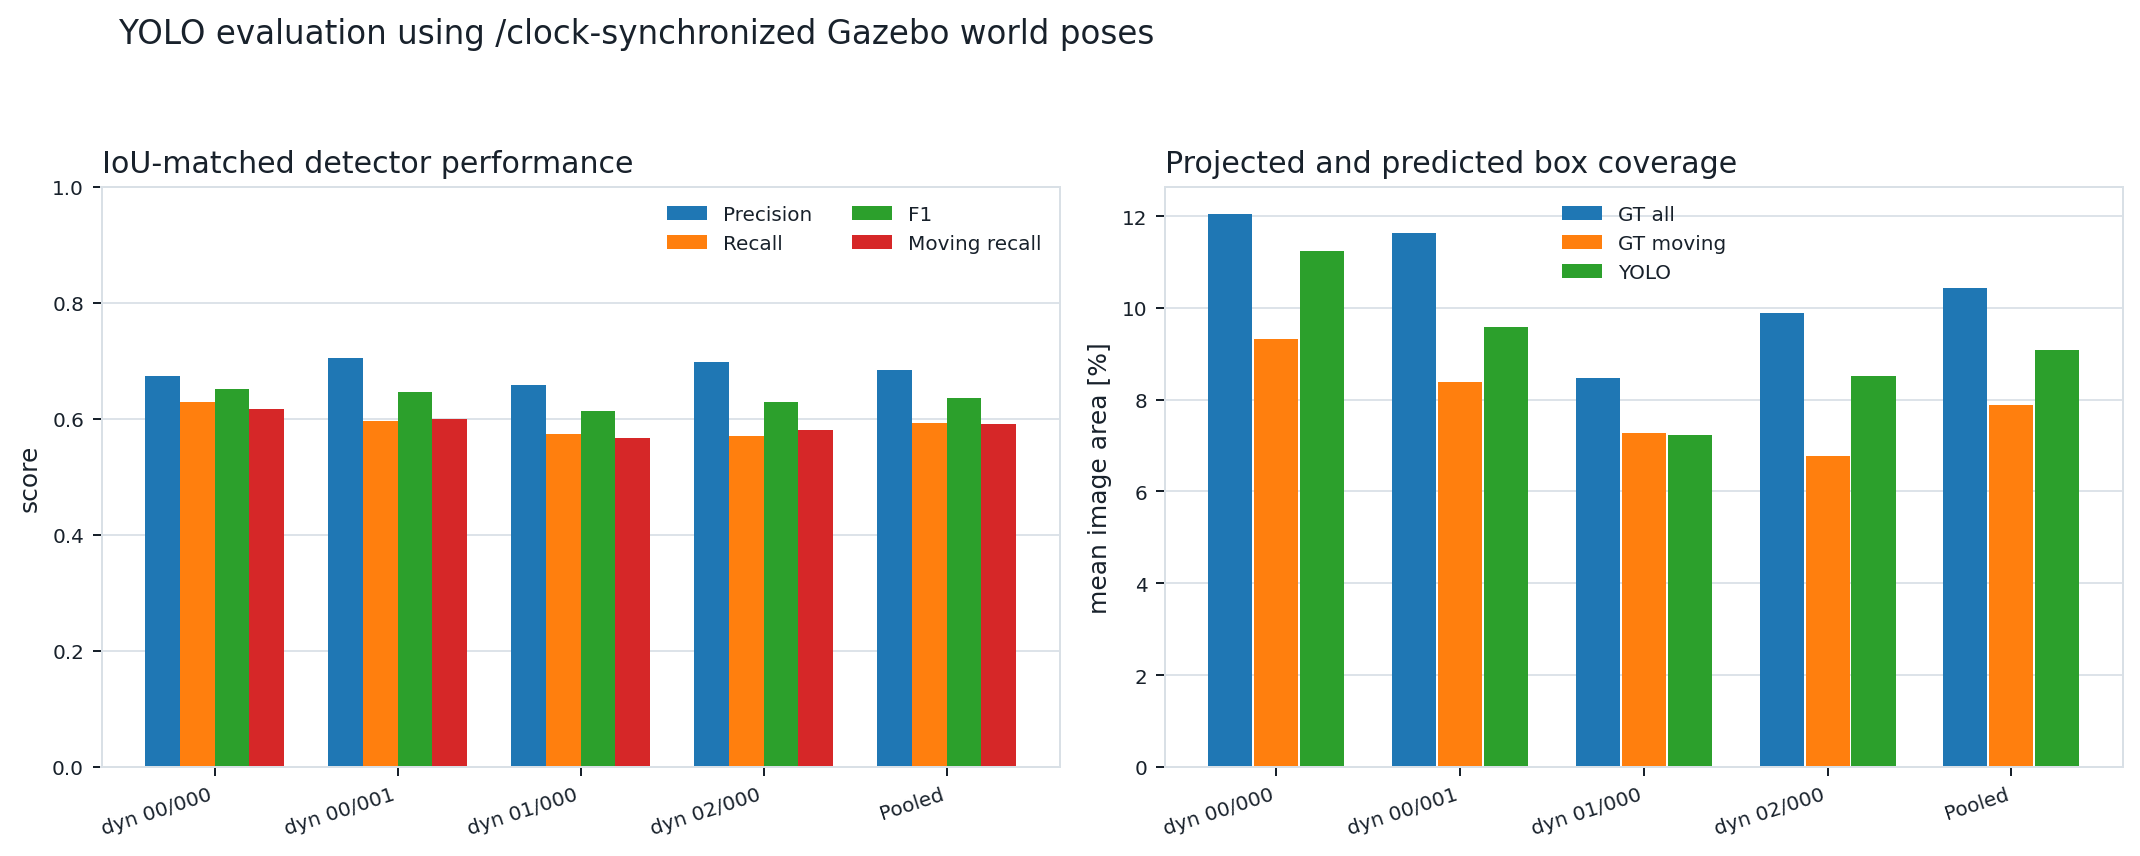
\includegraphics[width=\textwidth]{../../../output/yolo_eval/summary_light.png}
  \caption{Per-dataset and pooled detector scores and box-area coverage. Pooled
  precision, recall, F1, and moving-object recall are calculated from pooled
  counts, rather than by averaging the four displayed dataset scores.}
  \label{fig:yolo-performance-summary}
\end{figure}

\begin{figure}[htbp]
  \centering
  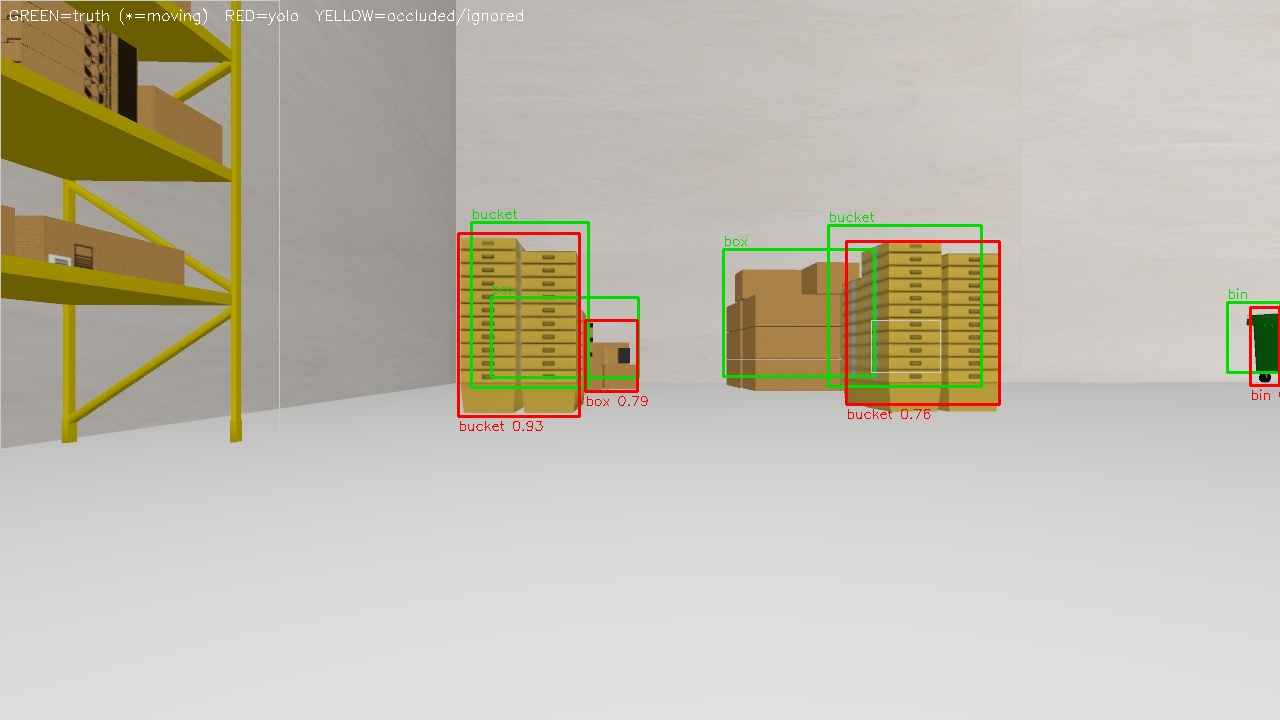
\includegraphics[width=\textwidth]{../../../output/yolo_eval/dyn_00_001/overlay/01116.jpg}
  \caption{Representative validation overlay used before accepting the offline
  metrics. Green boxes are projected ground truth, red boxes are YOLO
  predictions, and yellow boxes are occluded or ignored regions. An asterisk
  marks a ground-truth object classified as moving from its world-pose history.}
  \label{fig:yolo-ground-truth-overlay}
\end{figure}

\clearpage
\subsection{Object-Class Assignment Conditional on Localization}
\label{sec:yolo-classification}

This experiment is not whole-image classification: an image can contain many
objects, and the model outputs a class for each predicted bounding box. To keep
class assignment separate from localization, predictions and ground-truth boxes
were greedily associated by IoU $\geq0.50$ without requiring their classes to
agree. Classification was then evaluated only on the 37,061 localized object
pairs. Missed ground-truth objects and unmatched predictions remain bounding-box
detection errors in Section~\ref{sec:yolo-bbox}; they are not treated as an
additional semantic class here.

\begin{table}[htbp]
\centering
\caption{Object-class assignment conditional on successful IoU association,
pooled across the four dynamic datasets.}
\label{tab:yolo-classification}
\begin{tabular}{lrrrr}
\toprule
Class & Associated objects & Precision & Recall & F1 \\
\midrule
Bin & 2,639 & 1.000 & 1.000 & 1.000 \\
Box & 28,076 & 0.996 & 0.999 & 0.998 \\
Bucket & 6,346 & 0.996 & 0.983 & 0.989 \\
\midrule
Macro average & 37,061 & 0.997 & 0.994 & 0.995 \\
\bottomrule
\end{tabular}
\end{table}

The conditional class accuracy is 0.996: 36,924 of 37,061 associated objects
are on the confusion-matrix diagonal, leaving 137 class substitutions. The
largest substitution is 110 buckets labelled as boxes. This high conditional
accuracy does not cancel the weaker bounding-box recall: an object that was
never localized cannot enter the conditional class-assignment evaluation.

\begin{figure}[htbp]
  \centering
  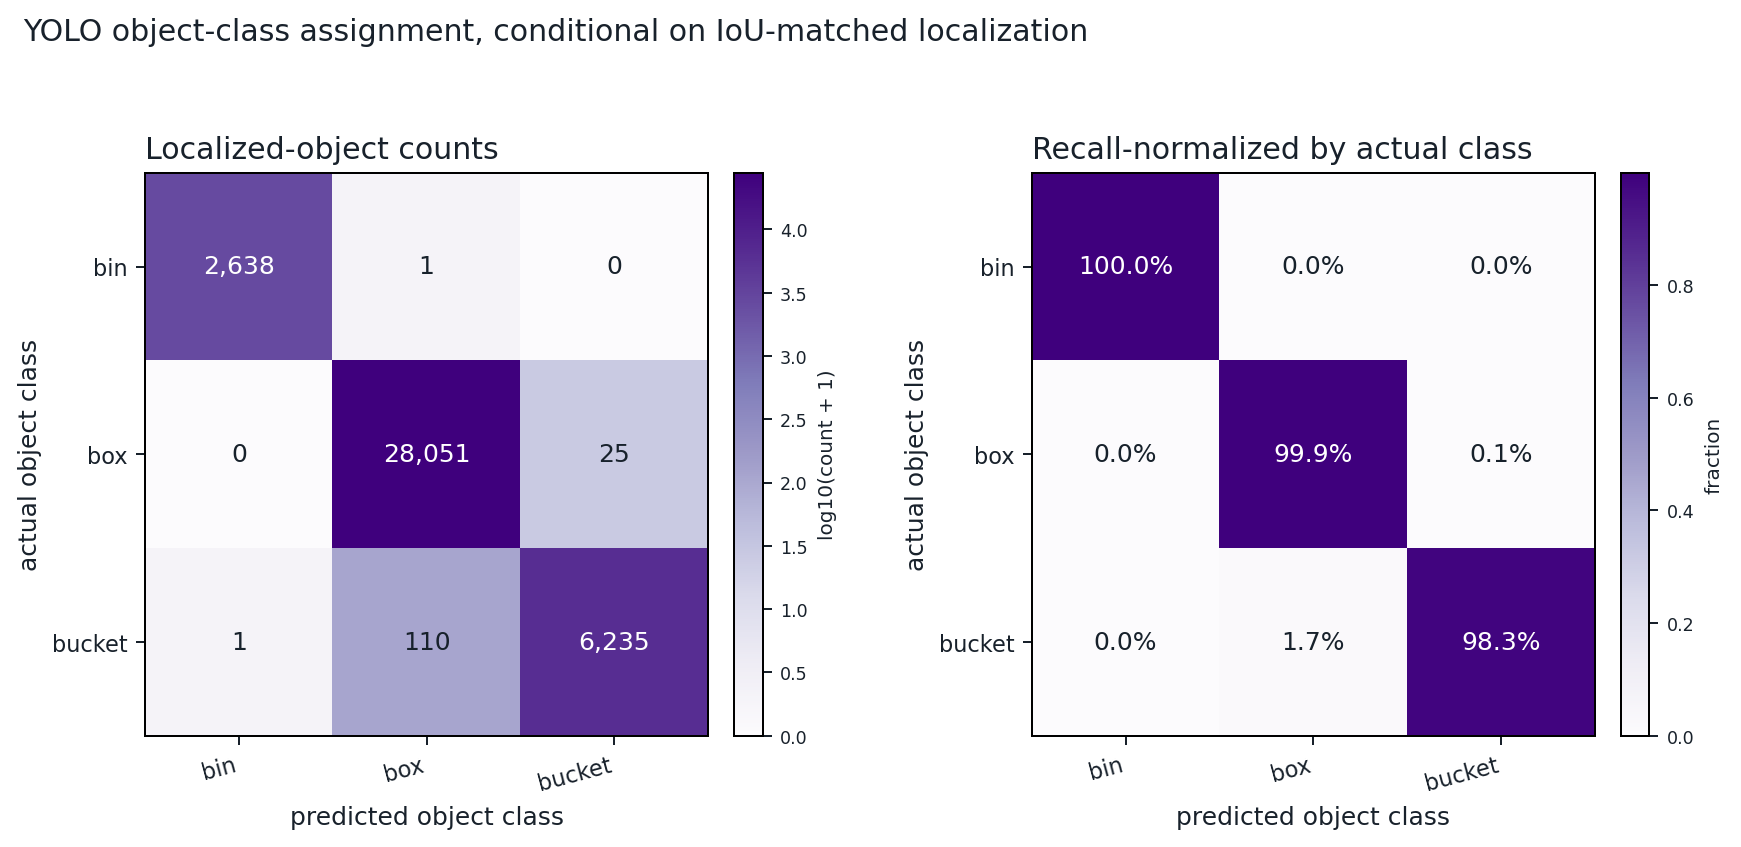
\includegraphics[width=\textwidth]{../../../output/yolo_eval/classification_confusion_light.png}
  \caption{Object-class confusion conditional on class-agnostic IoU association.
  Rows are actual object classes and columns are predicted object classes. The
  left panel gives counts on a logarithmic colour scale; the right panel
  normalizes within each actual class. Background is intentionally excluded.}
  \label{fig:yolo-classification-confusion}
\end{figure}

\section{Observed Anomaly Catalogue}
\label{sec:anomaly-catalogue}

Table~\ref{tab:anomaly-catalogue} records anomalous behaviour visible in the
logs and derived metrics. It deliberately separates observation from causal
explanation: no item below identifies a root cause, and the possible mechanisms
listed in the analysis catalogue remain untested.

\begingroup
\small
\setlength{\tabcolsep}{4pt}
% longtable captions default to 4in, which sets this one in a narrow indented
% block instead of across the table.
\setlength{\LTcapwidth}{\textwidth}
% Column widths plus 8 inter-column gaps must not exceed \textwidth, or the
% table is set into the right margin.
\begin{longtable}{p{0.05\textwidth}p{0.10\textwidth}p{0.26\textwidth}p{0.50\textwidth}}
\caption{Anomaly catalogue for the relogged campaign. Severity prioritizes
impact on interpretation, not certainty about cause.}
\label{tab:anomaly-catalogue}\\
\toprule
ID & Severity & Observation & Quantitative evidence and reporting consequence \\
\midrule
\endfirsthead
\toprule
ID & Severity & Observation & Quantitative evidence and reporting consequence \\
\midrule
\endhead
A1 & Critical & Requested VINS+YOLO filtering was inactive & All 12 folders contain
28,038 mask rows in total, but zero matched detector messages, positive-box
rows, or nonzero-coverage rows. They cannot measure an active semantic-filter
treatment. \\
A2 & High & ORB+YOLO exposure varied between repeats & Positive-box fractions
range from 1.4\% to 99.2\%, including wide variation among repeats of the same
bag. A matched detector message can contain zero boxes, so match count alone is
not treatment dose. \\
A3 & Critical & Every dynamic trajectory contains discontinuities & All 48
dynamic runs contain impossible-speed steps. Median affected-step fractions are
59.6\% (VINS), 30.3\% (ORB), 61.1\% (requested VINS+YOLO), and 26.9\%
(ORB+YOLO). Global ATE cannot be read as ordinary drift. \\
A4 & High & Global and clean-segment errors are strongly separated & Median
global-to-clean ATE ratios are 100, 146, 101, and 239 respectively. Locally
coherent intervals coexist with catastrophic full-run discontinuities. \\
A5 & Medium & Static ORB has an isolated initialization-adjacent jump & All nine
static ORB runs have one or two jumps, with the first near 2.6~s. Where an
inertial transition timestamp exists, the jump precedes it by 0.10--0.17~s;
this temporal association does not establish causation. \\
A6 & Medium & Two ORB run summaries are incomplete & The two static repeat
summaries omit final inertial/map fields, although frame and local-mapping logs
record initialized operation. Summary-only validation would falsely exclude
these runs. \\
A7 & High & ORB baseline/filter inputs are not paired in 11 of 12 cases & Invalid
pairs differ in received-frame count by 9.95--30.06\%, while their durations
differ by less than 0.13\%. Most between-mode differences are descriptive, not
controlled treatment effects. \\
A8 & Medium & VINS reset counts are non-discriminating & All 33 VINS baseline
and requested-filter runs have failure detection disabled and record zero
resets. Zero resets therefore cannot establish healthy estimation. \\
\bottomrule
\end{longtable}
\endgroup

\begin{figure}[htbp]
  \centering
  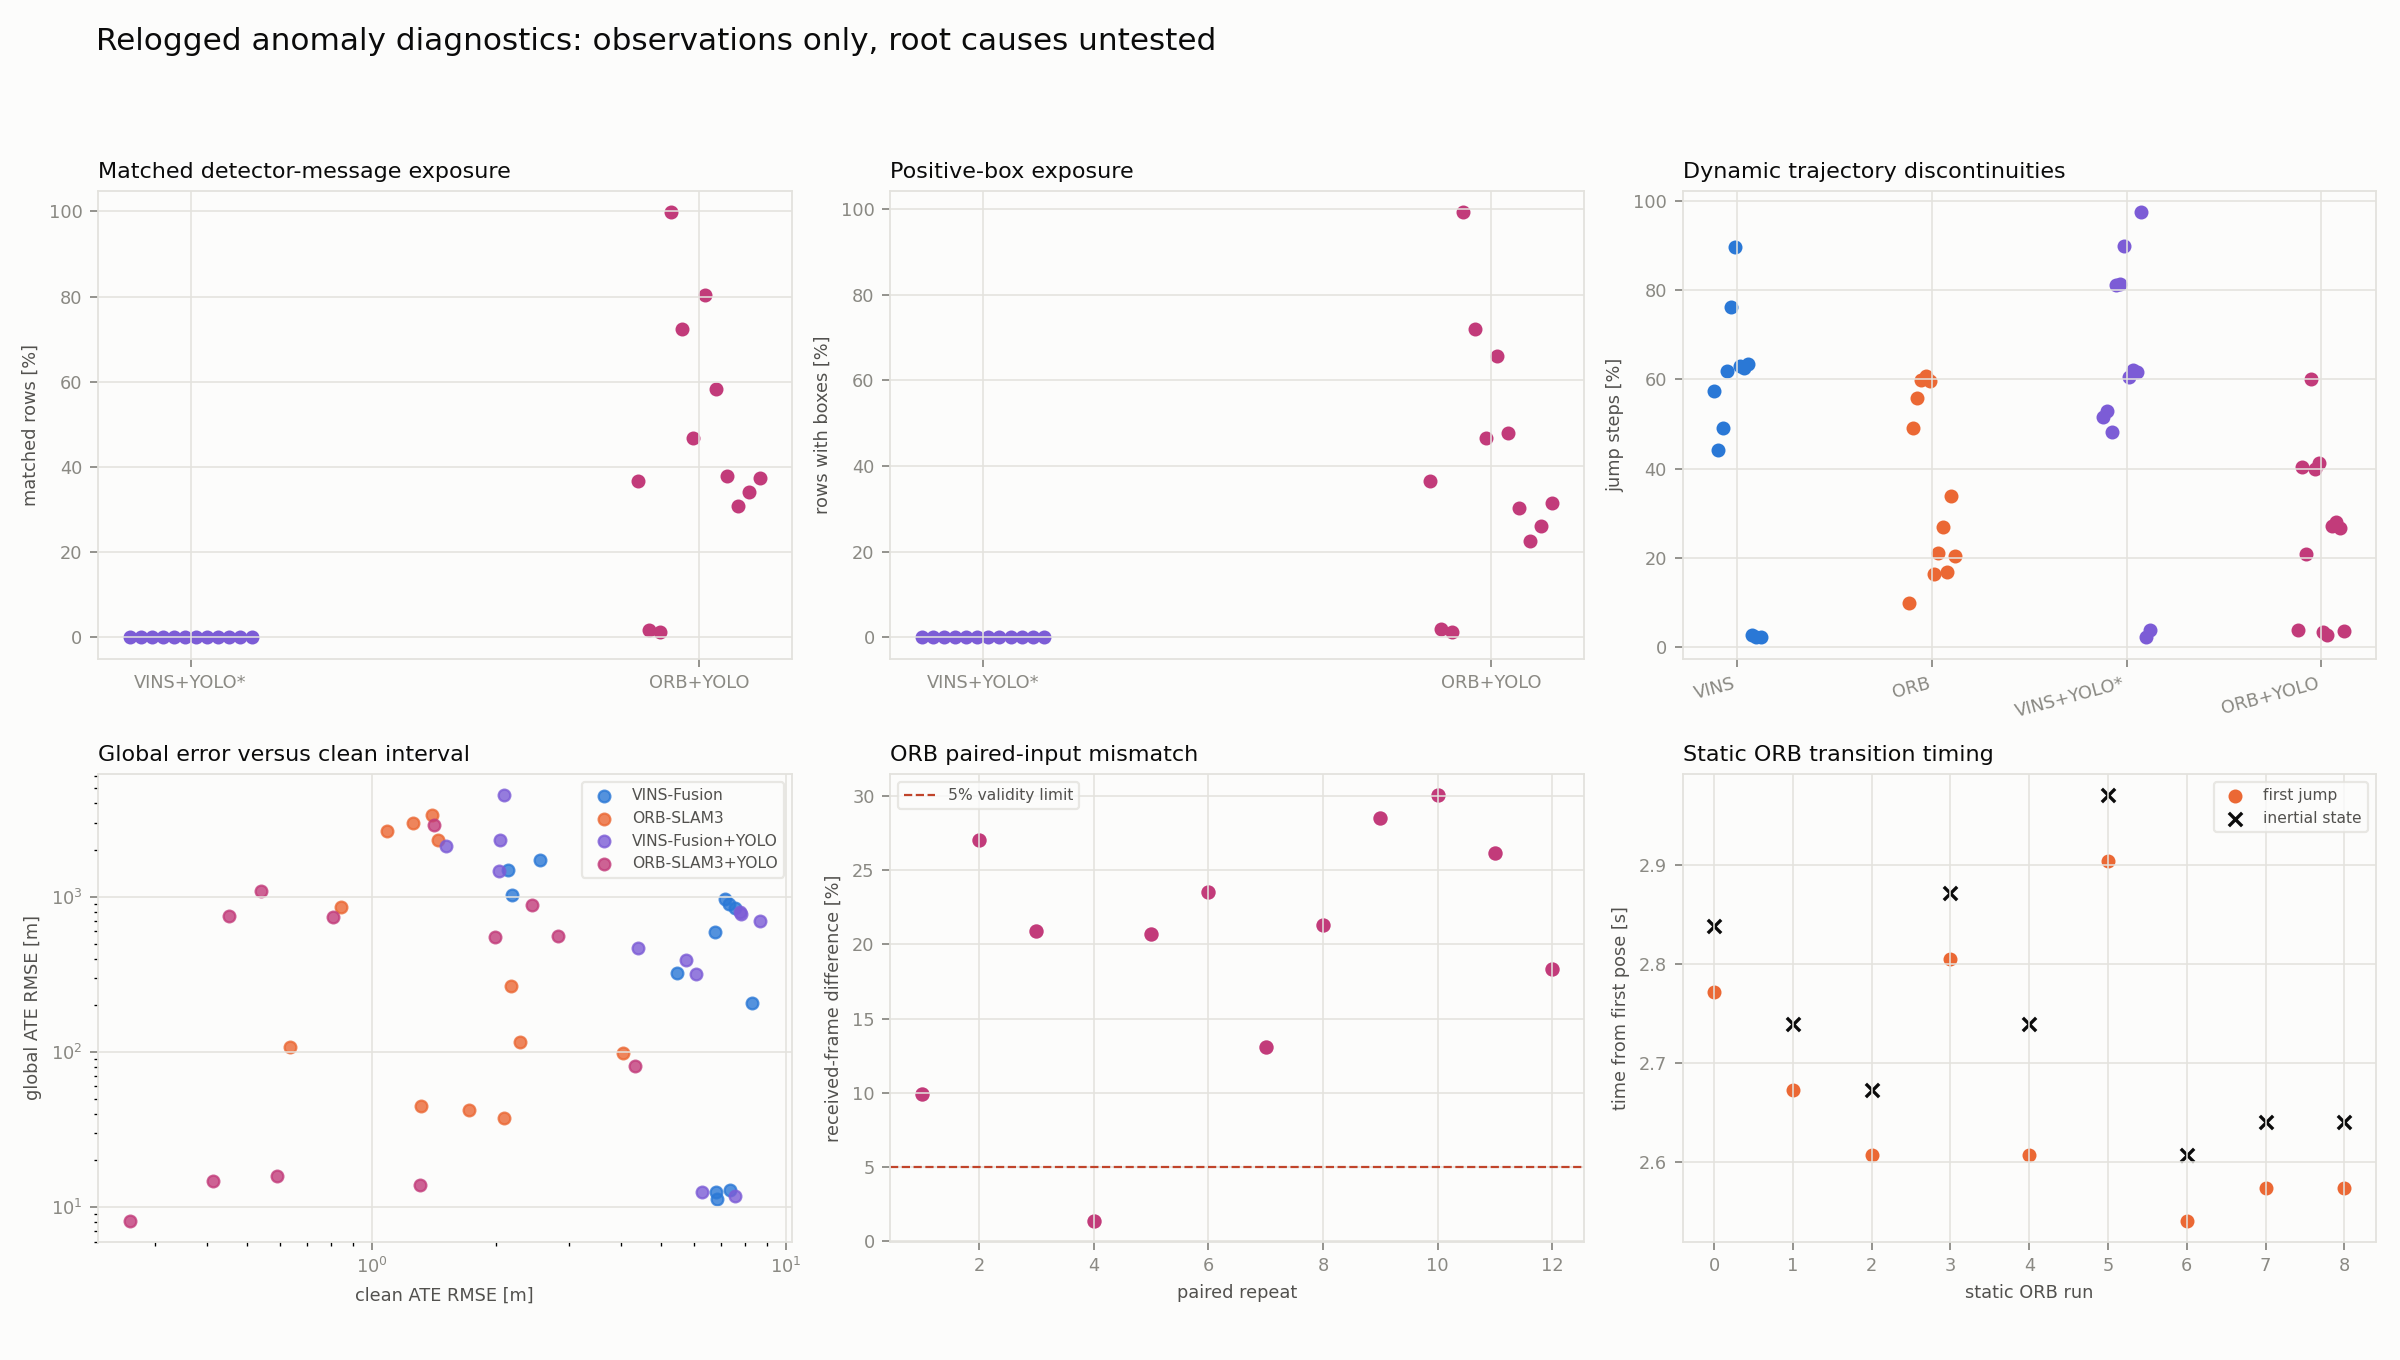
\includegraphics[width=\textwidth]{../../../output/compare/relogged_20260916/anomaly_diagnostics_light.png}
  \caption{Run-level anomaly diagnostics. The panels show detector-message and
  positive-box exposure, dynamic jump fractions, global versus clean-segment
  ATE, ORB paired-input mismatch, and static ORB jump timing. These are
  observations only; the plot does not assign a root cause.}
  \label{fig:anomaly-diagnostics}
\end{figure}

\section{Trajectory Accuracy, Plausibility, and Robustness}
\label{sec:trajectory-results}

\begin{queried}[Excluded: dynamic-scene trajectory results]
Every dynamic-scene trajectory result in this section, and the anomalies A3 and
A4 that derive from them, are \textbf{withheld as findings} and retained only as
excluded evidence. The reason is the environment, not the measurement: the
dynamic worlds move their props along scripted kinematic paths. The props carry
collision geometry but produce no dynamic response against the robot, nothing
constrains their speeds or routes to warehouse traffic, and they can occupy the
same space as the vehicle without consequence. Numbers measured there describe
the simulation, not the problem the thesis poses.

The runs happened, the artifacts are intact, and the plausibility failures are
real properties of those recordings, so they are reported below rather than
deleted --- an excluded measurement that explains a methodological correction is
worth more in the record than a gap. What must not be done is to read them as
evidence about estimator behaviour in a dynamic warehouse.

Two consequences follow. The condition this work is named for currently has no
valid testbed: it is untested, not tested and failed. And the environment becomes
the leading candidate explanation for the breakdown itself, displacing the
open question left in \cref{sec:anomaly-catalogue} --- testable by rebuilding the
worlds with physically simulated props and re-running, which requires no change
to either estimator.

Unaffected: the static-scene results here, the estimator comparison of
\cref{sec:results-proprio}, the detector evaluation of
\cref{sec:yolo-performance} --- prop motion is kinematic, which changes contact
physics rather than appearance, so detectability and class assignment are
untouched --- and the map evaluation of \cref{sec:map-quality}.
\end{queried}

Table~\ref{tab:trajectory-errors} reports medians and IQRs because the dynamic-run
distributions are strongly skewed. In static scenes, VINS attained a median
translational ATE RMSE of \SI{0.370}{\metre} and rotational RMSE of
\SI{1.56}{\degree} over nine valid runs. The nine valid static ORB runs attained
\SI{0.454}{\metre} and \SI{17.92}{\degree}. The orientation difference is much
larger than the positional difference and must be retained as a separate result.
\Cref{sec:rpe} shows that it is produced almost entirely by one or two discrete
events per run rather than by continuously worse orientation tracking.

\begin{table}[htbp]
\centering
\caption{Trajectory error against rosbag ground truth, median (IQR). ``Clean'' is
ATE RMSE after independently aligning the longest segment without an implied
speed above \SI{10}{\metre\per\second}. Requested VINS+YOLO values are not
active-filter measurements.}
\label{tab:trajectory-errors}
\resizebox{\textwidth}{!}{%
\begin{tabular}{llrrrr}
\toprule
Scene & Requested mode & ATE RMSE (m) & Rotation RMSE (deg) & Clean ATE (m) & Jumps \\
\midrule
Static & VINS-Fusion & $0.370\;(0.063)$ & $1.56\;(0.98)$ & $0.370\;(0.063)$ & $0\;(0)$ \\
Static & ORB-SLAM3 & $0.454\;(0.157)$ & $17.92\;(1.72)$ & $0.341\;(0.151)$ & $1\;(1)$ \\
Dynamic & VINS-Fusion & $724.13\;(823.52)$ & $53.97\;(39.38)$ & $6.80\;(2.57)$ & $1116\;(1157.75)$ \\
Dynamic & ORB-SLAM3 & $190.48\;(2315.44)$ & $108.29\;(116.13)$ & $1.42\;(0.89)$ & $484\;(418.5)$ \\
Dynamic & VINS-Fusion+YOLO$^{*}$ & $738.63\;(1251.84)$ & $56.50\;(37.88)$ & $5.91\;(5.53)$ & $1559.5\;(717)$ \\
Dynamic & ORB-SLAM3+YOLO & $556.05\;(769.39)$ & $138.42\;(60.34)$ & $1.06\;(1.58)$ & $208\;(225.5)$ \\
\bottomrule
\multicolumn{6}{l}{$^{*}$Filter requested but no detection frame was matched.}
\end{tabular}}
\end{table}

Every dynamic run contains at least one impossible-speed step. Nine of 12
baseline VINS runs, all 12 baseline ORB runs, 10 of 12 nominal VINS+YOLO runs,
and all 12 ORB+YOLO runs also exceeded the reference-free mean-speed limit of
\SI{3}{\metre\per\second}. Peak translational error exceeded \SI{50}{\metre} in
9, 12, 10, and 10 runs respectively. Global ATE is therefore dominated by
trajectory breakdown. The clean-segment ATE is substantially smaller, which an
earlier draft read as evidence that the runs contain locally coherent intervals.
\Cref{sec:rpe} withdraws that reading: measured directly, the jump-free
relative error is \SIrange{1.8}{3.8}{\metre} per second, so the estimate is
locally wrong by more than the distance the robot travels. Aligning a short
segment absorbs much of that error, which is why clean-segment ATE looked
reassuring.

The per-repeat values behind those aggregates are given in
\cref{tab:truth-summary}.

\subsection{Relative pose error}
\label{sec:rpe}

RPE was implemented after the reporting cutoff and applied to the campaign
without re-running any estimator; \cref{sec:method-trajectory} defines it. It is
reported here because it needs no global alignment, so unlike ATE it cannot be
distorted by a single discontinuity re-seating the rigid fit.
\Cref{tab:rpe-summary} gives the headline interval.

\begin{table}[htbp]
\centering
\caption{Relative pose error at $\Delta=\SI{1}{\second}$, median (IQR) over runs.
``Jump-free'' excludes pairs spanning a detected tracking jump; the difference
between the two columns is the teleport contribution. Requested VINS+YOLO values
are not active-filter measurements.}
\label{tab:rpe-summary}
\footnotesize
\setlength{\tabcolsep}{3pt}
% Generated by script/make_result_tables.py from
% output/compare/relogged_20260916/trajectory_metrics.csv.
% Do not edit by hand; regenerate instead.
\begin{tabular}{llrrrrr}
\toprule
& & & \multicolumn{2}{c}{Translational (m)} & \multicolumn{2}{c}{Rotational (deg)} \\
\cmidrule(lr){4-5}\cmidrule(lr){6-7}
Scene & Requested mode & Jumps & all pairs & jump-free & all pairs & jump-free \\
\midrule
Static & VINS-Fusion & 0\,(0) & 0.063\,(0.027) & 0.063\,(0.027) & 0.57\,(0.05) & 0.57\,(0.05) \\
Static & ORB-SLAM3 & 1\,(1) & 0.310\,(0.308) & 0.096\,(0.064) & 10.56\,(0.69) & 0.25\,(0.33) \\
\midrule
Dynamic & VINS-Fusion & 1116\,(1158) & 44.652\,(49.397) & 2.825\,(1.595) & 2.05\,(1.63) & 2.76\,(2.01) \\
Dynamic & ORB-SLAM3 & 484\,(418) & 19.477\,(158.567) & 2.079\,(0.267) & 15.15\,(4.82) & 2.49\,(2.51) \\
Dynamic & VINS-Fusion+YOLO$^{*}$ & 1560\,(717) & 44.106\,(95.564) & 3.784\,(1.611) & 2.33\,(4.76) & 2.72\,(1.02) \\
Dynamic & ORB-SLAM3+YOLO & 208\,(226) & 38.174\,(78.432) & 1.805\,(0.634) & 21.60\,(9.72) & 6.33\,(10.39) \\
\bottomrule
\end{tabular}

\end{table}

Two results follow, and the first corrects this chapter.

\paragraph{The dynamic runs are not locally coherent.} Excluding every pair that
spans a jump, dynamic translational RPE at $\Delta=\SI{1}{\second}$ is still
\SIrange{1.8}{3.8}{\metre}. The robot covers about \SI{1.4}{\metre} in that
second, so between teleports the estimate misstates its own motion by more than
the distance travelled. Against the static runs, whose jump-free figures are
\SIrange{0.063}{0.096}{\metre}, dynamic local error is \num{20} to \num{60}
times worse. The corruption is therefore continuous, not confined to isolated
steps, and the earlier reading of clean-segment ATE as evidence of local
coherence does not survive. This was a registered prediction before the metric
was run, and it failed in the direction that matters.

\begin{table}[htbp]
\centering
\caption{Jump-free translational RPE against interval, median over runs, in
metres. ``Growth'' is the ratio from \SI{0.5}{\second} to \SI{5}{\second};
linear accumulation would give \num{10}$\times$ and a pure random walk
\num{3.2}$\times$.}
\label{tab:rpe-sweep}
\small
\setlength{\tabcolsep}{5pt}
% Generated by script/make_result_tables.py from
% output/compare/relogged_20260916/trajectory_metrics.csv.
% Do not edit by hand; regenerate instead.
\begin{tabular}{llrrrrr}
\toprule
Scene & Requested mode & \SI{0.5}{\second} & \SI{1.0}{\second} & \SI{2.0}{\second} & \SI{5.0}{\second} & Growth \\
\midrule
Static & VINS-Fusion & 0.038 & 0.063 & 0.112 & 0.252 & 6.7$\times$ \\
Static & ORB-SLAM3 & 0.057 & 0.096 & 0.162 & 0.307 & 5.4$\times$ \\
\midrule
Dynamic & VINS-Fusion & 1.524 & 2.825 & 5.067 & 10.082 & 6.6$\times$ \\
Dynamic & ORB-SLAM3 & 1.158 & 2.079 & 3.776 & 6.787 & 5.9$\times$ \\
Dynamic & VINS-Fusion+YOLO$^{*}$ & 2.189 & 3.784 & 5.455 & 10.985 & 5.0$\times$ \\
Dynamic & ORB-SLAM3+YOLO & 0.976 & 1.805 & 3.041 & 4.384 & 4.5$\times$ \\
\bottomrule
\end{tabular}

\end{table}

\Cref{tab:rpe-sweep} shows why this is one mechanism rather than two. Error grows
with interval at \numrange{4.5}{6.7}$\times$ over a tenfold increase in
$\Delta$, and that growth exponent is the same for static and dynamic scenes;
only the magnitude differs, by roughly \num{40}$\times$. The dynamic runs are
not failing in a qualitatively different way from the static ones --- they are
running the same error process far hotter.

\paragraph{ORB-SLAM3's static rotational penalty is entirely jump-localised.}
Static ORB-SLAM3 carries a rotational ATE of \SI{17.92}{\degree} against
VINS-Fusion's \SI{1.56}{\degree}, an elevenfold gap that invites the reading
that ORB-SLAM3 tracks orientation poorly. RPE refutes it. Across the nine static
ORB runs, all-pairs rotational RPE is \SIrange{9.28}{11.63}{\degree}, but
jump-free rotational RPE is \SIrange{0.10}{0.66}{\degree} --- at or below
VINS-Fusion's \SIrange{0.49}{0.69}{\degree} on the same recordings. Every one of
those runs contains one or two jumps and no more.

The whole rotational gap is thus produced by one or two discrete re-seating
events per run, not by continuously worse tracking. This gives anomaly~A5 its
significance: that jump occurs near \SI{2.6}{\second}, immediately before
inertial initialization completes, and it is predominantly rotational. Between
those events ORB-SLAM3's orientation tracking is competitive with VINS-Fusion's.
No causal mechanism is established here --- the association is temporal --- but
the error is now localized to an event rather than attributed to the estimator's
steady-state behaviour.

\begin{sidewaystable}[p]
\centering
\caption{Truth-based trajectory error for every repeat of the relogged
campaign. Every dataset is a no-floor-texture world, so that shared part of each
dataset name is omitted. ``ATE'' and ``clean'' are global and
longest-clean-segment ATE RMSE in metres, ``rot'' is rotational geodesic RMSE in
degrees, and ``jmp'' counts steps implying more than \SI{10}{\metre\per\second}.
All 66 runs are operational; two static ORB run summaries have incomplete
schemas, and only one of 12 ORB baseline/filter pairs passed input matching.
Static datasets were not run in either filtered mode; those cells are set to --.}
\label{tab:truth-summary}
\scriptsize
\setlength{\tabcolsep}{4pt}
% Generated by script/make_result_tables.py from
% output/compare/relogged_20260916/trajectory_metrics.csv.
% Do not edit by hand; regenerate instead.
\begin{tabular}{llrrrrrrrrrrrrrrrr}
\toprule
& & \multicolumn{4}{c}{VINS-Fusion} & \multicolumn{4}{c}{ORB-SLAM3} & \multicolumn{4}{c}{VINS-Fusion+YOLO$^{*}$} & \multicolumn{4}{c}{ORB-SLAM3+YOLO} \\
\cmidrule(lr){3-6}\cmidrule(lr){7-10}\cmidrule(lr){11-14}\cmidrule(lr){15-18}
Dataset & Rep & ATE & rot & clean & jmp & ATE & rot & clean & jmp & ATE & rot & clean & jmp & ATE & rot & clean & jmp \\
& & (m) & (deg) & (m) & (n) & (m) & (deg) & (m) & (n) & (m) & (deg) & (m) & (n) & (m) & (deg) & (m) & (n) \\
\midrule
dynamic 00\_000 & 01 & 596.37 & 38.5 & 6.77 & 858 & 45.21 & 176.5 & 1.31 & 109 & 392.55 & 107.0 & 5.74 & 1122 & 13.84 & 76.7 & 1.31 & 37 \\
dynamic 00\_000 & 02 & 206.97 & 92.2 & 8.32 & 609 & 857.95 & 162.0 & 0.84 & 512 & 466.72 & 108.0 & 4.39 & 1183 & 892.31 & 129.9 & 2.45 & 213 \\
dynamic 00\_000 & 03 & 324.01 & 88.4 & 5.47 & 580 & 3364.34 & 70.8 & 1.40 & 610 & 318.66 & 108.7 & 6.07 & 991 & 81.20 & 173.1 & 4.33 & 119 \\
dynamic 00\_001 & 01 & 1030.40 & 63.6 & 2.18 & 1374 & 3002.57 & 29.7 & 1.26 & 1150 & 2309.93 & 74.6 & 2.04 & 1805 & 2885.77 & 82.2 & 1.42 & 1159 \\
dynamic 00\_001 & 02 & 1481.00 & 62.8 & 2.14 & 1695 & 2669.73 & 26.1 & 1.09 & 1141 & 2129.97 & 75.2 & 1.51 & 1810 & 553.35 & 93.5 & 1.98 & 454 \\
dynamic 00\_001 & 03 & 1724.94 & 175.1 & 2.55 & 1995 & 2311.30 & 23.1 & 1.45 & 1098 & 1457.89 & 59.6 & 2.03 & 1997 & 558.76 & 112.8 & 2.82 & 378 \\
dynamic 01\_000 & 01 & 904.94 & 53.3 & 7.29 & 1608 & 98.88 & 169.1 & 4.05 & 239 & 698.15 & 52.0 & 8.67 & 1545 & 8.20 & 102.3 & 0.26 & 44 \\
dynamic 01\_000 & 02 & 851.90 & 53.8 & 7.55 & 1596 & 115.45 & 172.4 & 2.28 & 327 & 796.03 & 52.6 & 7.77 & 1582 & 14.78 & 173.8 & 0.41 & 26 \\
dynamic 01\_000 & 03 & 965.82 & 54.1 & 7.14 & 1619 & 107.60 & 167.7 & 0.64 & 456 & 779.10 & 53.3 & 7.79 & 1574 & 749.16 & 162.6 & 0.45 & 203 \\
dynamic 02\_000 & 01 & 12.49 & 6.1 & 6.80 & 72 & 37.83 & 59.3 & 2.09 & 388 & 4518.77 & 25.1 & 2.09 & 2610 & 1097.95 & 159.7 & 0.54 & 231 \\
dynamic 02\_000 & 02 & 12.88 & 5.5 & 7.36 & 61 & 265.50 & 62.9 & 2.17 & 689 & 11.85 & 6.4 & 7.55 & 62 & 737.27 & 148.9 & 0.81 & 219 \\
dynamic 02\_000 & 03 & 11.30 & 4.3 & 6.81 & 58 & 42.37 & 145.8 & 1.72 & 408 & 12.55 & 6.9 & 6.29 & 66 & 15.81 & 146.9 & 0.59 & 31 \\
\midrule
static 000 & 01 & 0.37 & 1.6 & 0.37 & 0 & 0.58 & 17.9 & 0.55 & 1 & -- & -- & -- & -- & -- & -- & -- & -- \\
static 000 & 02 & 0.41 & 1.5 & 0.41 & 0 & 0.79 & 20.4 & 0.77 & 1 & -- & -- & -- & -- & -- & -- & -- & -- \\
static 000 & 03 & 0.43 & 1.6 & 0.43 & 0 & 1.20 & 19.1 & 0.30 & 2 & -- & -- & -- & -- & -- & -- & -- & -- \\
static 001 & 01 & 0.39 & 2.3 & 0.39 & 0 & 0.45 & 18.9 & 0.27 & 2 & -- & -- & -- & -- & -- & -- & -- & -- \\
static 001 & 02 & 0.29 & 1.8 & 0.29 & 0 & 0.45 & 18.1 & 0.21 & 2 & -- & -- & -- & -- & -- & -- & -- & -- \\
static 001 & 03 & 0.48 & 2.2 & 0.48 & 0 & 0.38 & 17.2 & 0.26 & 1 & -- & -- & -- & -- & -- & -- & -- & -- \\
static 002 & 01 & 0.34 & 0.8 & 0.34 & 0 & 0.42 & 16.7 & 0.39 & 1 & -- & -- & -- & -- & -- & -- & -- & -- \\
static 002 & 02 & 0.36 & 0.8 & 0.36 & 0 & 0.46 & 17.6 & 0.43 & 1 & -- & -- & -- & -- & -- & -- & -- & -- \\
static 002 & 03 & 0.34 & 0.7 & 0.34 & 0 & 0.36 & 16.9 & 0.34 & 1 & -- & -- & -- & -- & -- & -- & -- & -- \\
\bottomrule
\end{tabular}


\vspace{1ex}
\raggedright\footnotesize
$^{*}$Filter requested but no detection frame was matched in any repeat; these
columns are not active-filter measurements.
\end{sidewaystable}

\begin{figure}[htbp]
  \centering
  % The summary table belongs with these panels, so it is set inside the float
  % rather than as a separate table that page-breaking could carry away.
  {\small\setlength{\tabcolsep}{3pt}% Generated by script/make_result_tables.py from
% output/compare/relogged_20260916/trajectory_metrics.csv.
% Do not edit by hand; regenerate instead.
\begin{tabular}{lrrrrrrr}
\toprule
Requested mode & Poses & Overlap & Path & ATE RMSE & Rot RMSE & Clean ATE & Jumps \\
& (n) & (s) & (m) & (m) & (deg) & (m) & (n) \\
\midrule
VINS-Fusion & 1494 & 77.0 & 5486.93 & 596.367 & 38.51 & 6.771 & 858 \\
ORB-SLAM3 & 1105 & 77.3 & 408.22 & 45.206 & 176.53 & 1.314 & 109 \\
VINS-Fusion+YOLO$^{*}$ & 2175 & 77.1 & 1958.14 & 392.546 & 107.04 & 5.743 & 1122 \\
ORB-SLAM3+YOLO & 943 & 77.2 & 239.53 & 13.839 & 76.72 & 1.310 & 37 \\
\bottomrule
\end{tabular}
}

  \vspace{0.5ex}
  {\footnotesize $^{*}$Filter requested but no detection frame was matched.}

  \vspace{2ex}
  % The image carries its own rendered title, the same summary table, and a
  % footnote in the top 310 px of 2496; that band is trimmed away because those
  % numbers are now typeset above.
  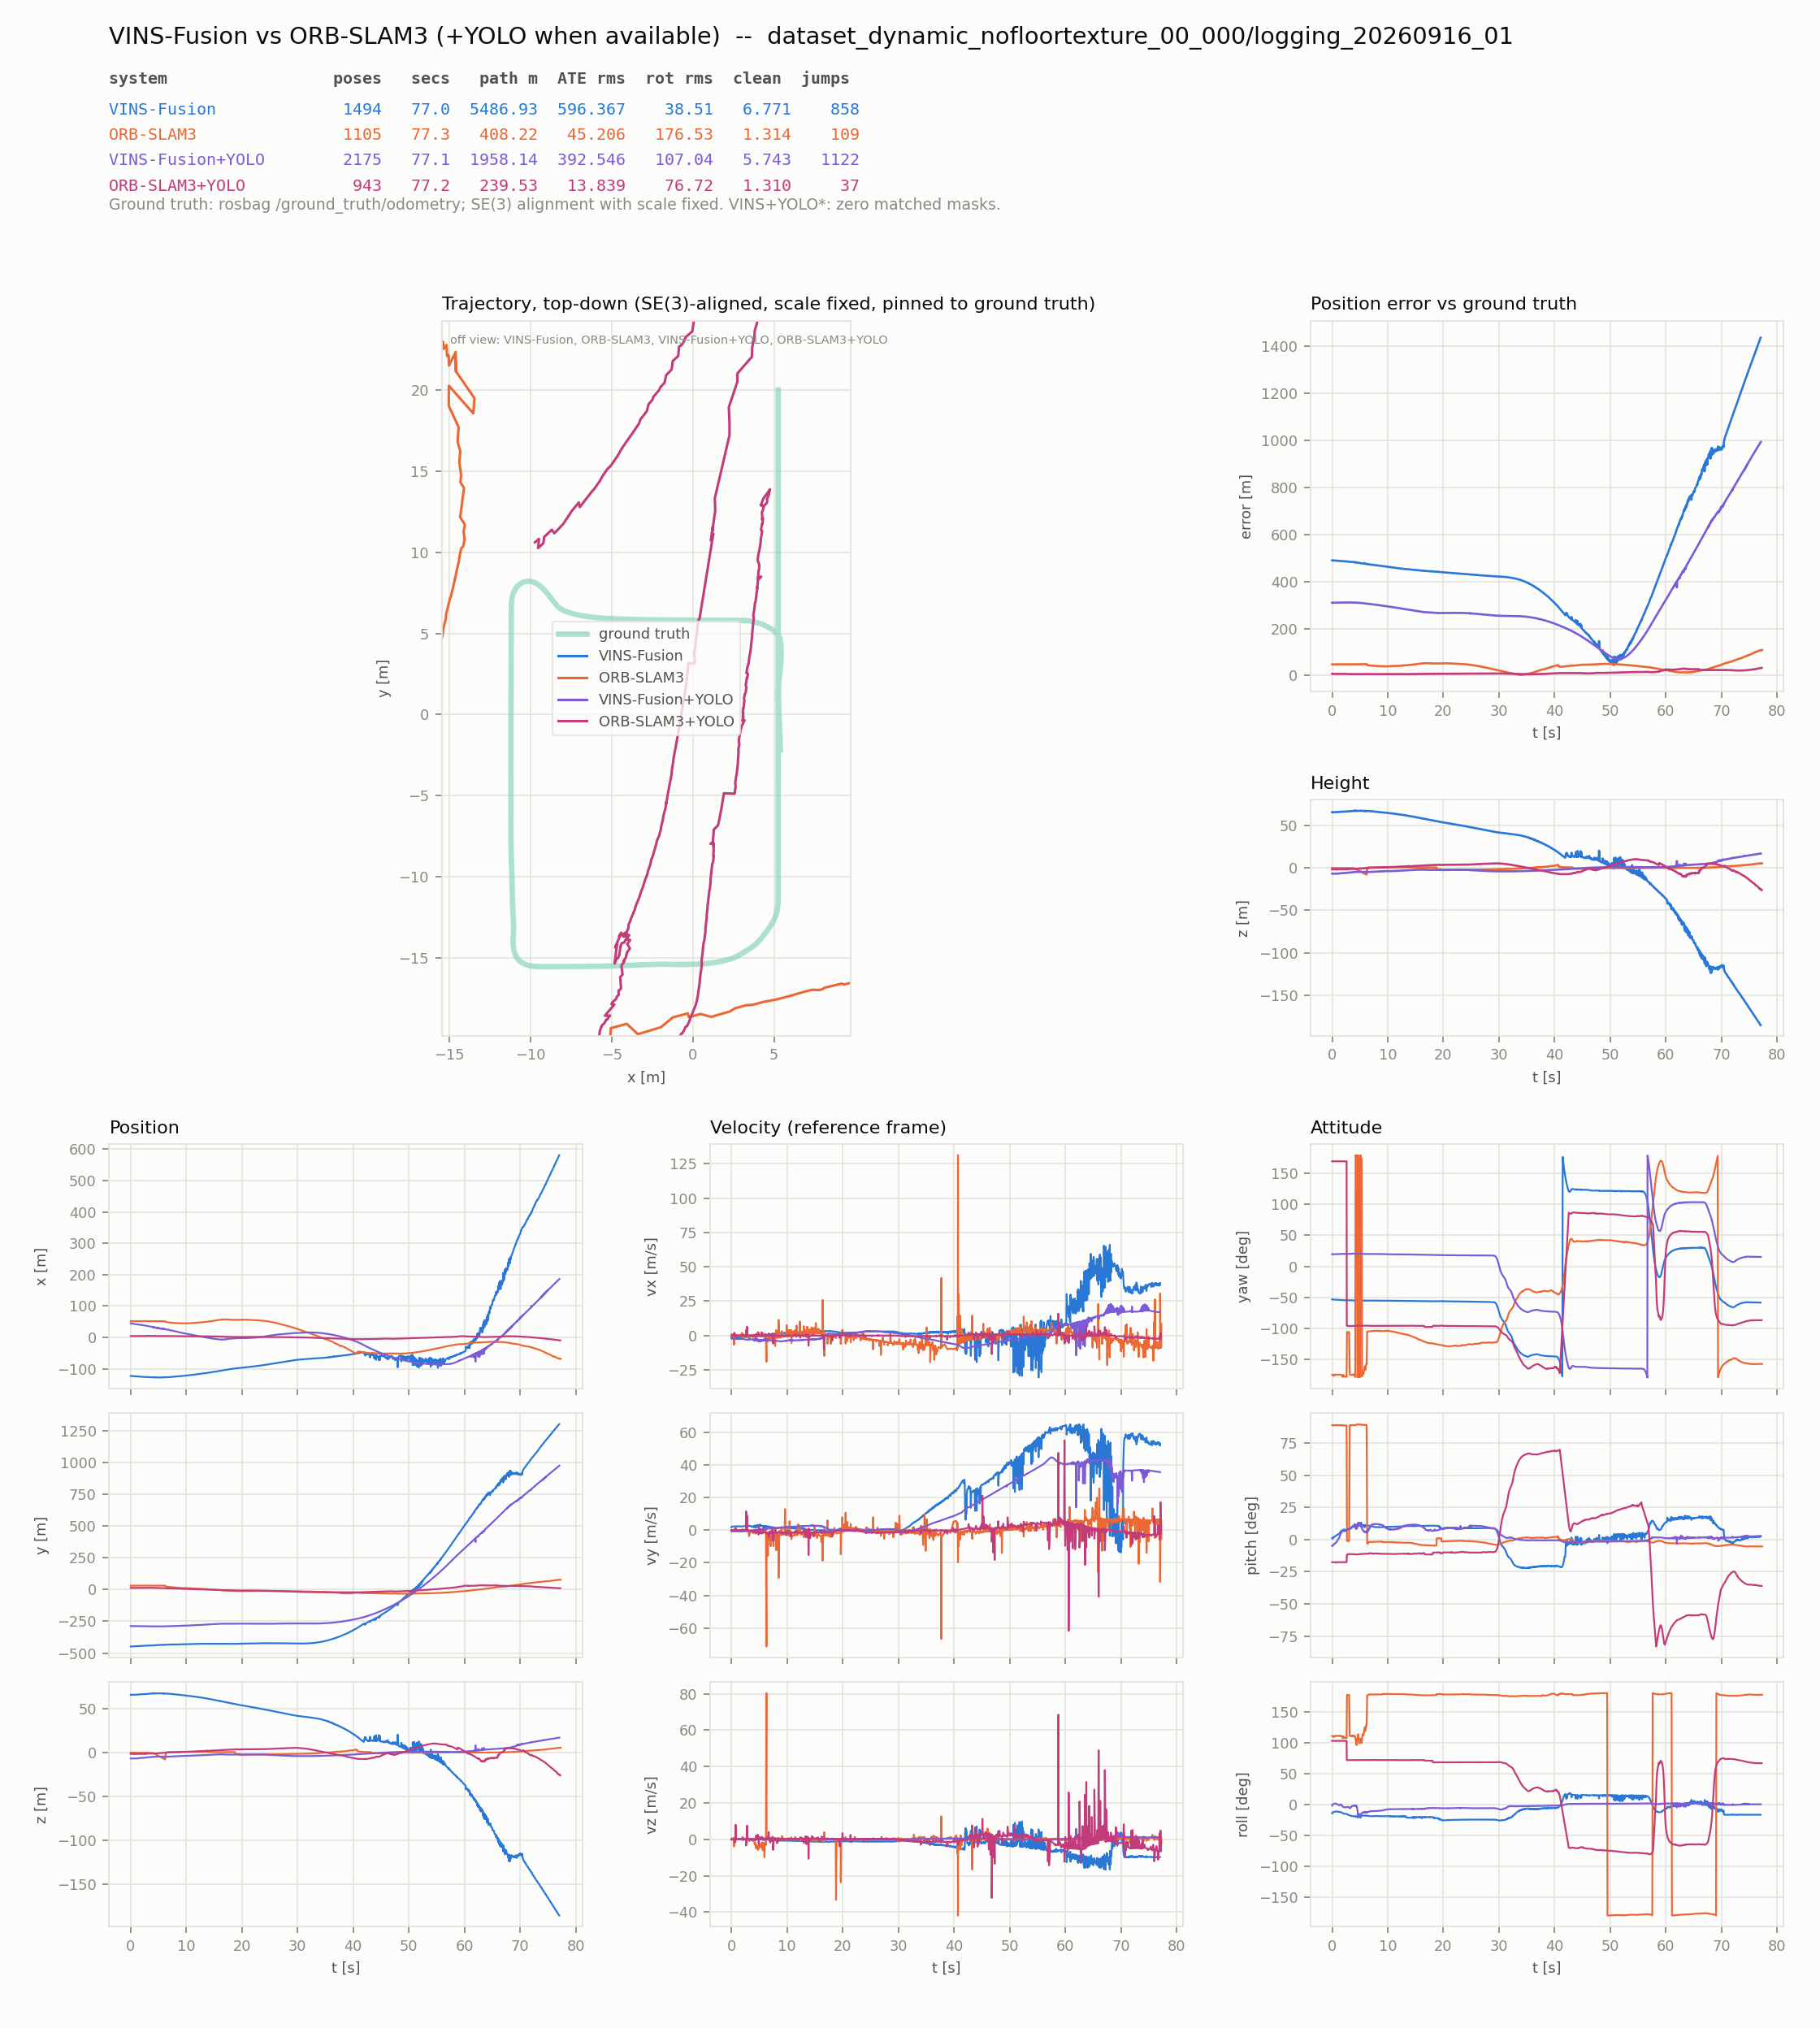
\includegraphics[width=\textwidth, trim={0 0 0 140pt}, clip]{../../../output/compare/relogged_20260916/simulation/dataset_dynamic_nofloortexture_00_000/logging_20260916_01/compare_light.png}
  \caption{Representative repeated-run trajectory diagnostic for
  \repo{dataset_dynamic_nofloortexture_00_000/logging_20260916_01}, in the same
  visual format as the existing comparison figures. The table gives the
  per-system summary for this run; ``clean'' is ATE RMSE over the longest
  jump-free segment. The very large paths and frequent jumps are retained rather
  than clipped into a favourable view. ATE and rotational errors use the rosbag
  \repo{/ground_truth/odometry} topic after rigid $SE(3)$ alignment with scale
  fixed. The nominal VINS+YOLO trace is invalid as a filtering treatment because
  no masks were matched.}
  \label{fig:relogged-trajectory-example}
\end{figure}

Baseline ORB-SLAM3 logged $7.75\pm6.03$ tracking-loss events and
$9.52\pm6.49$~s of lost tracking per dynamic run (mean $\pm$ sample SD,
$n=12$). ORB+YOLO logged $9.17\pm3.01$ events and $11.46\pm5.32$~s. VINS logged
no estimator resets in either requested mode, but the absence of resets does not
make its trajectories plausible. The event types are estimator-specific and are
not treated as numerically equivalent.

\begin{figure}[htbp]
  \centering
  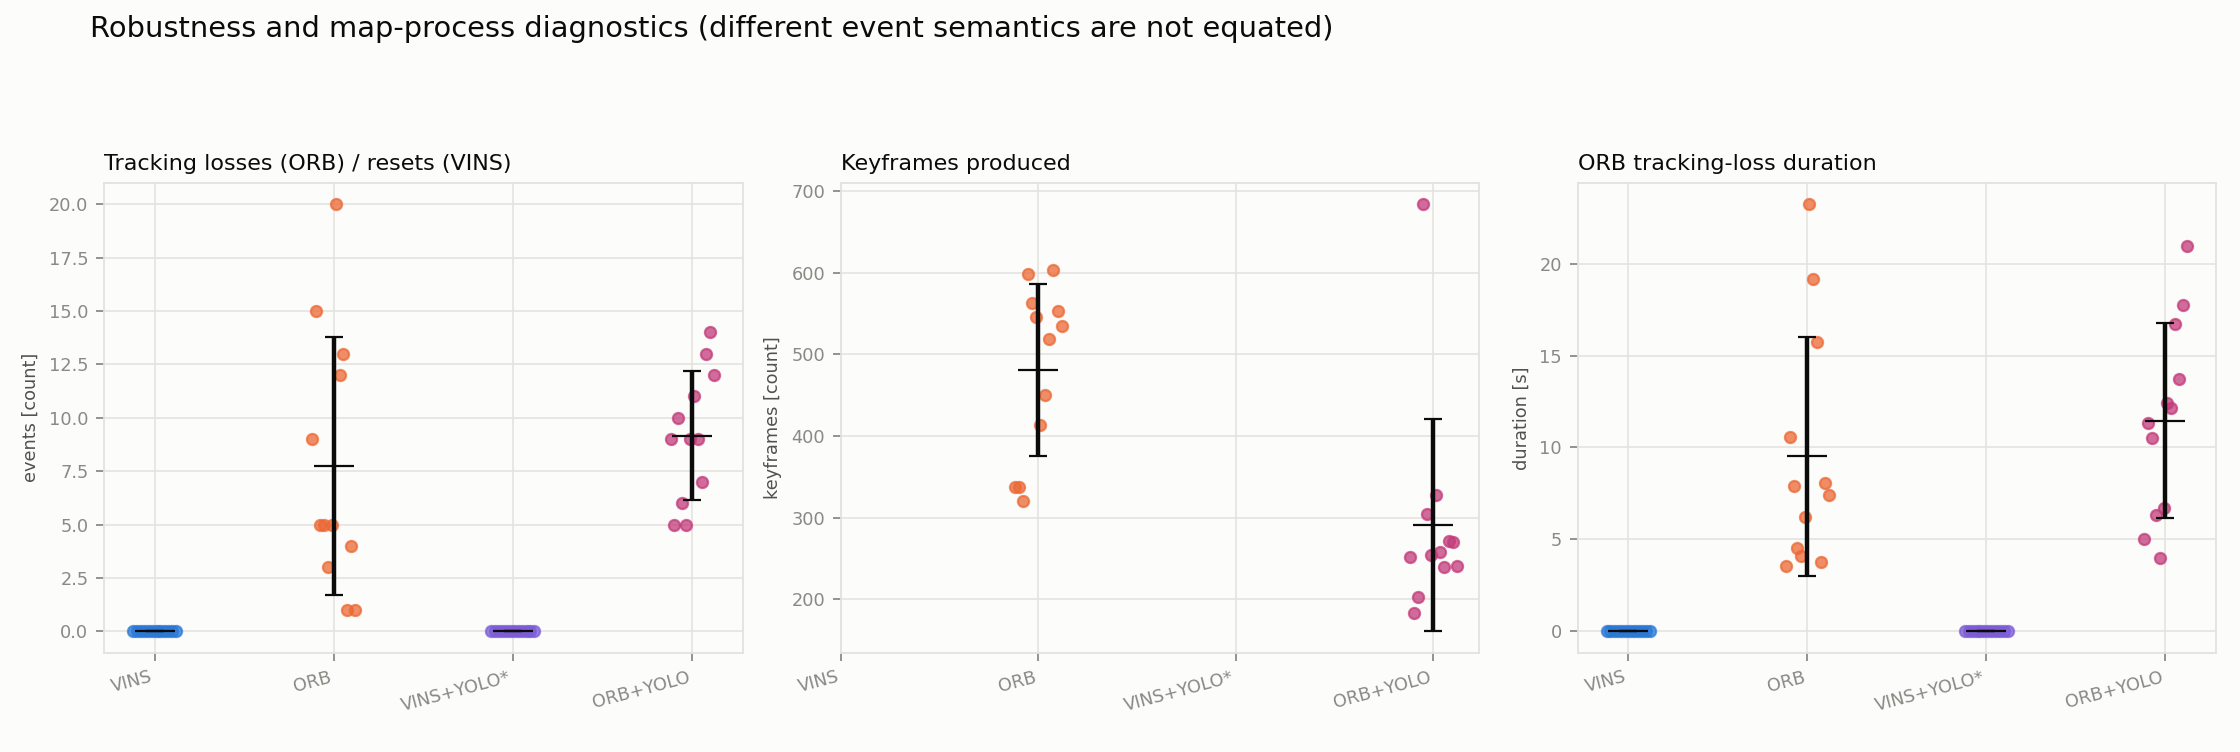
\includegraphics[width=\textwidth]{../../../output/compare/relogged_20260916/robustness_light.png}
  \caption{Per-run robustness and keyframe observations for the dynamic datasets.
  Points are experimental runs and black marks are mean $\pm$ sample SD. VINS
  reset count and ORB tracking-loss count have different semantics. The asterisk
  identifies the requested VINS filter mode in which no masks were matched.}
  \label{fig:robustness-results}
\end{figure}

\section{Real-Time and Computational Measurements}
\label{sec:compute-results}

Table~\ref{tab:capacity-results} summarizes process-local measurements over the
12 dynamic runs in each requested mode. CPU is the change in cumulative process
CPU time divided by monotonic wall time; 100\% denotes one fully used logical
core, so values above 100\% represent multithreaded execution. Memory is peak
resident set size. The separate detector process, rosbag, Gazebo, RViz, and
RTAB-Map are not included.

\begin{table}[htbp]
\centering
\caption{Dynamic-run capacity and resource measurements, mean $\pm$ sample SD,
$n=12$ per row. Nominal VINS+YOLO values are not active-filter measurements.}
\label{tab:capacity-results}
\resizebox{\textwidth}{!}{%
\begin{tabular}{lrrrr}
\toprule
Requested mode & Throughput (Hz) & Retained input (\%) & CPU (\% core) & Peak RSS (MiB) \\
\midrule
VINS-Fusion & $27.14\pm5.81$ & $100.00\pm0.00$ & $443.66\pm58.96$ & $629.51\pm282.62$ \\
ORB-SLAM3 & $23.47\pm4.77$ & $88.55\pm13.42$ & $385.22\pm27.71$ & $1226.06\pm81.83$ \\
VINS-Fusion+YOLO$^{*}$ & $28.83\pm3.16$ & $100.00\pm0.00$ & $406.43\pm89.95$ & $646.14\pm306.15$ \\
ORB-SLAM3+YOLO & $14.47\pm5.42$ & $66.96\pm15.26$ & $410.86\pm42.83$ & $1054.64\pm91.11$ \\
\bottomrule
\multicolumn{5}{l}{$^{*}$Filter requested but no detection frame was matched.}
\end{tabular}}
\end{table}

The ORB+YOLO folders show lower achieved throughput and retention than baseline
ORB, while process CPU is of similar order. This is an observation, not an
isolated detector-cost effect: the external detector is excluded from CPU and 11
paired runs received materially different image counts. Baseline VINS processed
all enqueued images in its logs, whereas baseline ORB discarded frames whenever
the one-frame queue was overwritten.

\begin{figure}[htbp]
  \centering
  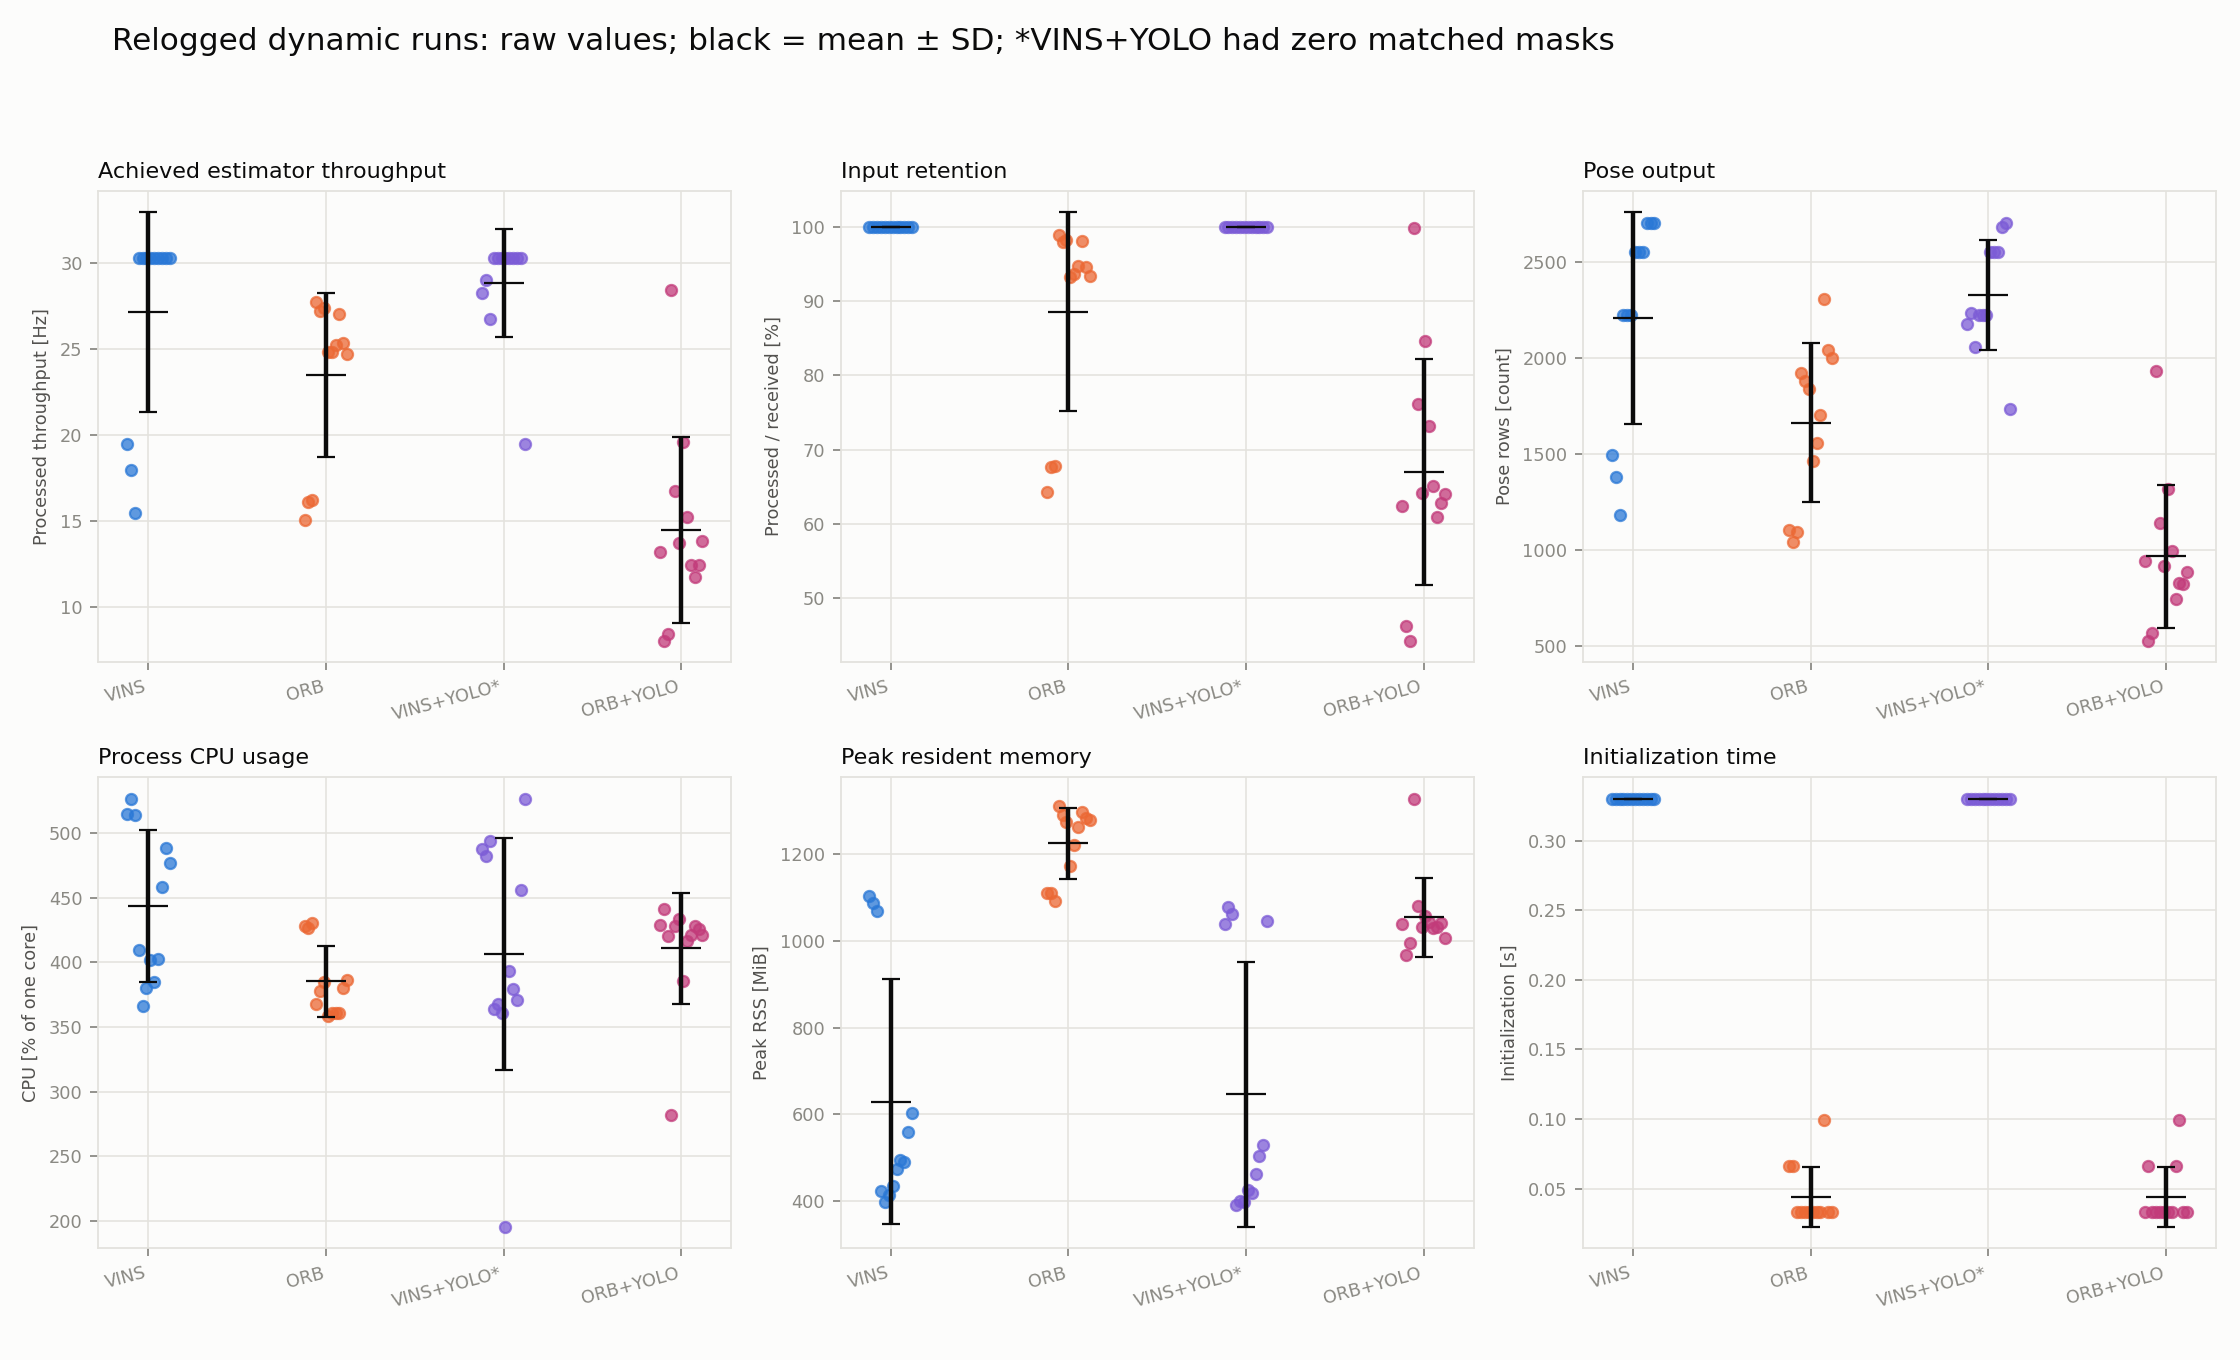
\includegraphics[width=\textwidth]{../../../output/compare/relogged_20260916/capacity_resources_light.png}
  \caption{Raw dynamic-run capacity and process-resource values. Each point is a
  run; black marks show mean $\pm$ sample SD. This plot exposes run-to-run spread
  rather than presenting only aggregate bars.}
  \label{fig:capacity-resources}
\end{figure}

Per-module results use each run's event distribution. Figure~\ref{fig:module-latency}
shows pooled event boxplots for shape, overlaid with one median point per run so
frames are not mistaken for independent experimental repeats. Across run medians,
ORB tracking was $63.19\pm7.06$~ms and ORB local mapping was
$189.58\pm16.95$~ms. The requested ORB+YOLO mode measured
$112.53\pm24.61$~ms and $356.30\pm68.36$~ms respectively. VINS feature tracking
was $48.00\pm10.83$~ms and its back end was $60.41\pm17.12$~ms; nominal
VINS+YOLO values were $43.61\pm11.49$~ms and $57.90\pm16.29$~ms, but cannot be
interpreted as filter effects because that filter was inactive. These timings
refer to different estimator stages and are not added or treated as directly
equivalent algorithms.

\begin{figure}[htbp]
  \centering
  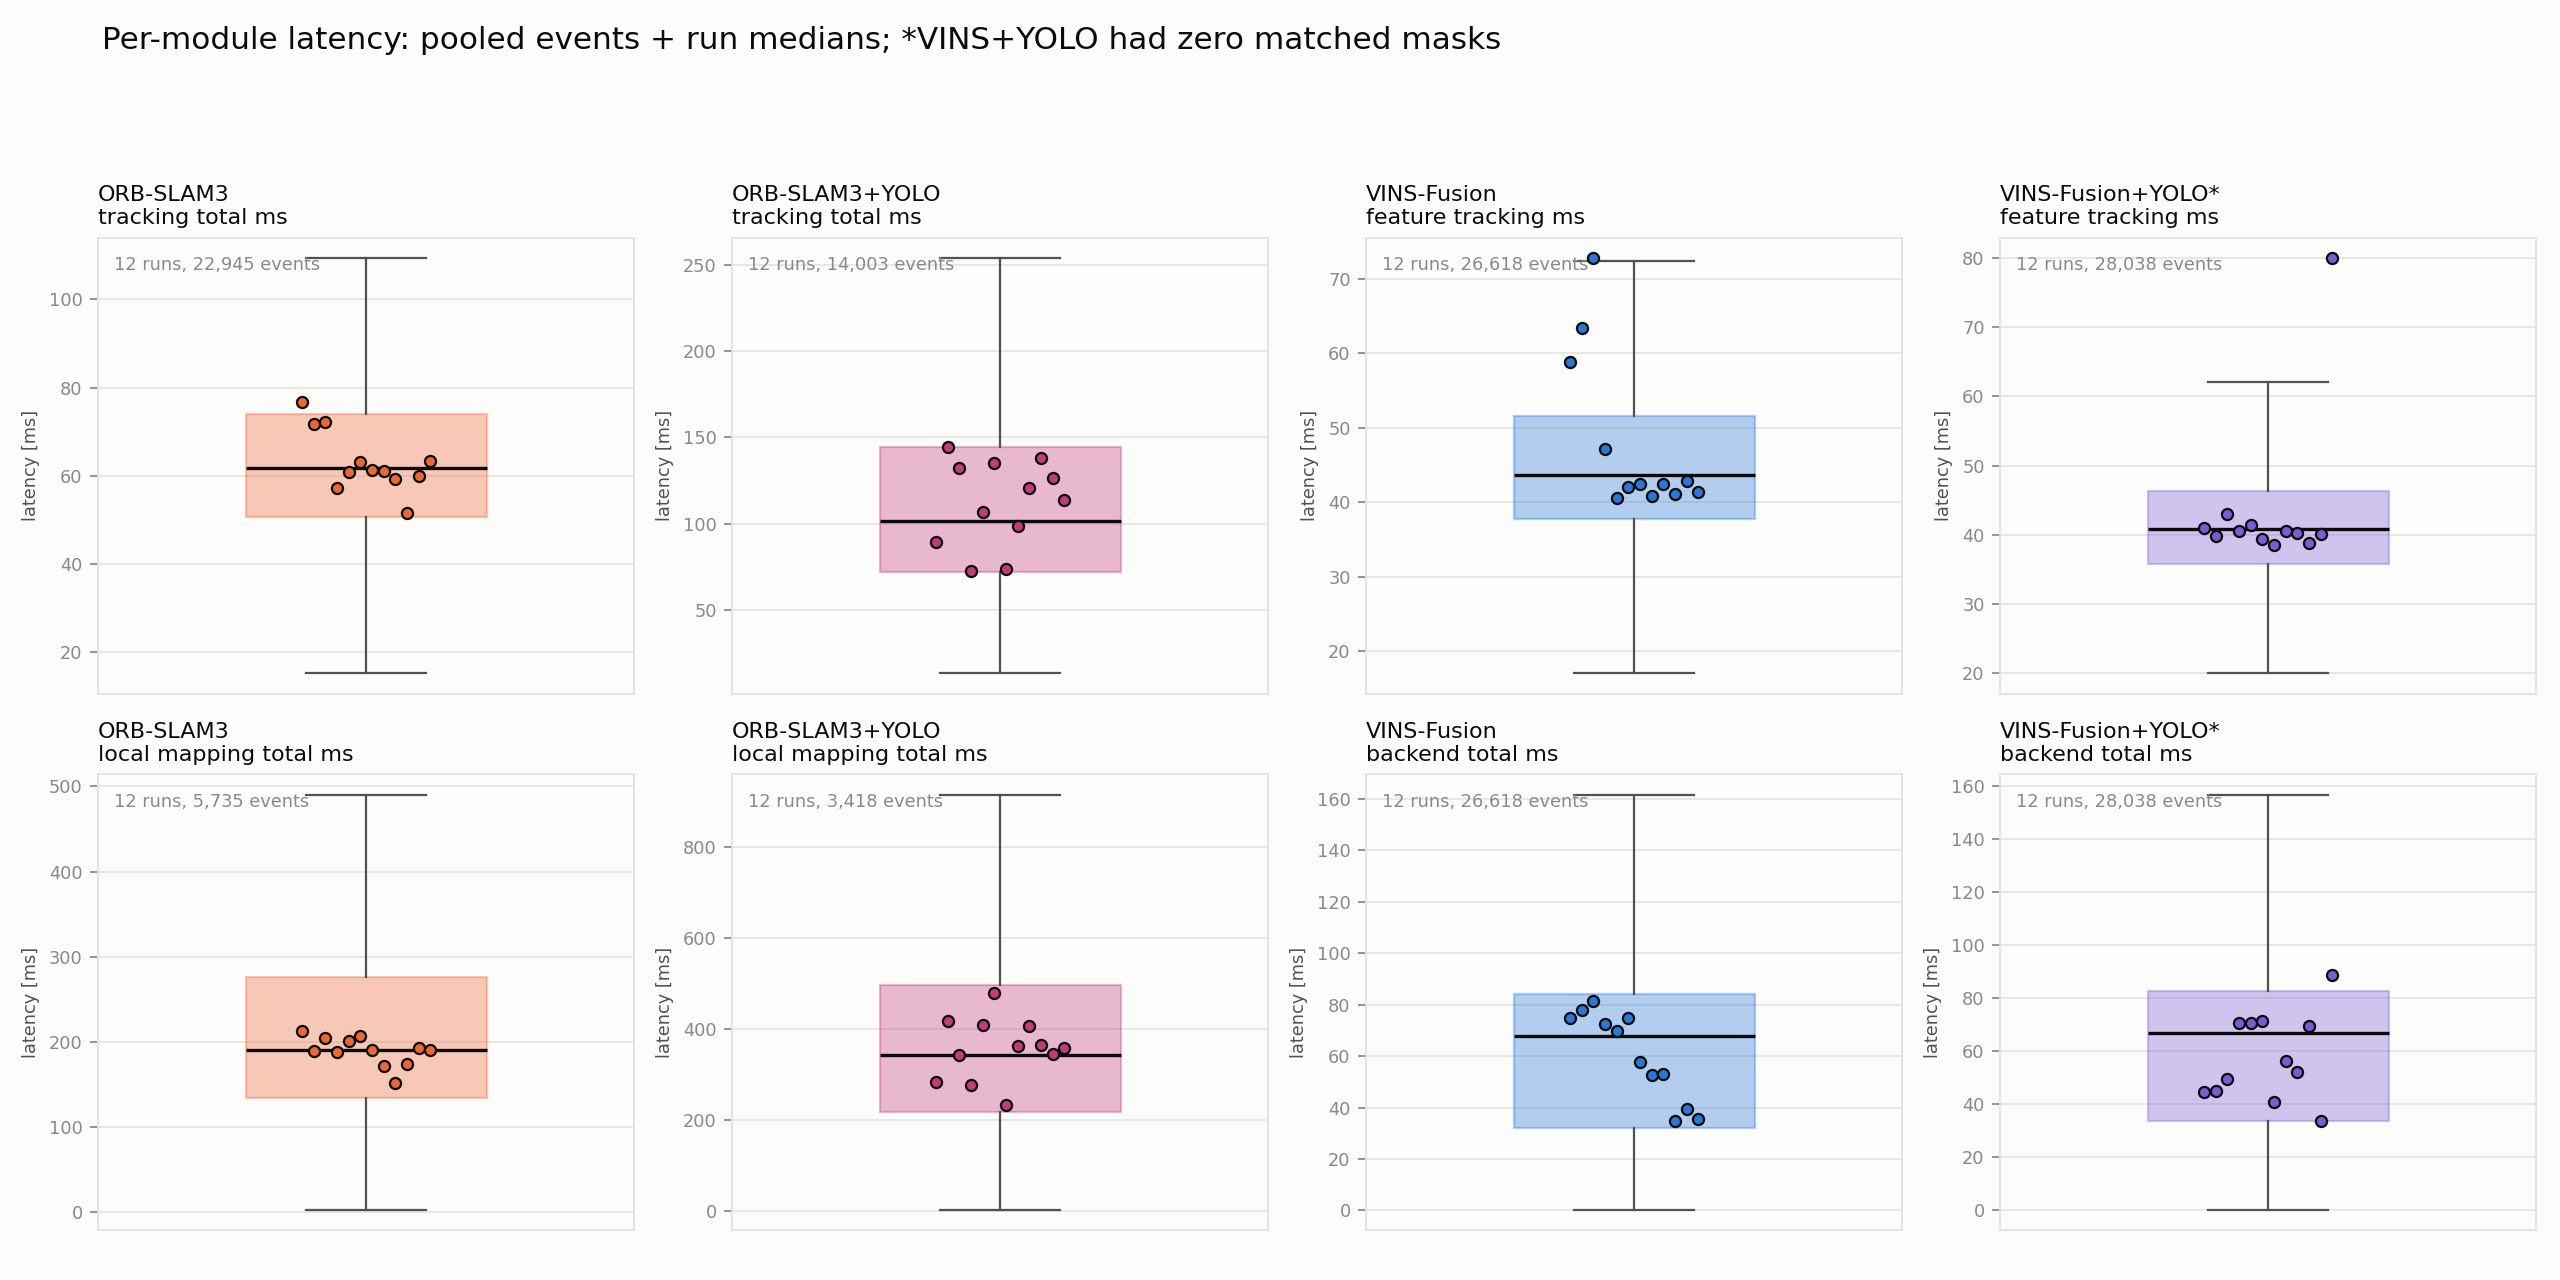
\includegraphics[width=\textwidth]{../../../output/compare/relogged_20260916/module_latency_light.png}
  \caption{Module-latency distributions for dynamic datasets. Boxes summarize
  all recorded module events; coloured points are per-run medians ($n=12$ in
  each requested mode). ORB local mapping is asynchronous per keyframe, while
  VINS back-end rows follow estimator updates.}
  \label{fig:module-latency}
\end{figure}

\clearpage
\section{Dense Map Reconstruction and Map-Quality Evaluation}
\label{sec:map-quality}

\subsection{Question, scope, and conditions}

Trajectory error answers whether the robot knew where it was. It does not answer
whether the map it produced describes the building, nor whether a planner could
have used that map. This section evaluates the one dense map reconstructed so far
against two references of very different strength: the simulator's own collision
geometry, which is independent of the map, and the ground-truth route of the run
that built the map, which is not. The two questions are kept separate because
they fail in different ways --- a map can be geometrically faithful and still
unusable, and it can be navigable over an easy route while misrepresenting the
parts of the building that route never entered --- and because only the first
reference is independent evidence.

The evaluation is confined to the \textbf{tiny} warehouse. A large-warehouse
equivalent is \status{planned}; no database for it exists at the reporting
cutoff. Tiny-map and large-map results must not be pooled or read as repeated
trials of one condition, because the two worlds differ in extent, aisle width,
and route length. \Cref{tab:map-conditions} records the conditions.

\begin{table}[htbp]
\centering
\caption{Conditions for the dense-map evaluation. The database and the
ground-truth route come from the \emph{same} run, which bounds what the
drivability figures can establish.}
\label{tab:map-conditions}
\small
\begin{tabularx}{\textwidth}{>{\raggedright\arraybackslash}p{0.26\textwidth}>{\raggedright\arraybackslash}X}
\toprule
Factor & Level \\
\midrule
Map under test & \repo{map/map_tiny.db}, RTAB-Map 0.23.7, created 2026-09-08 \\
World &
  \repo{aws-robomaker-small-warehouse-world/worlds/small_warehouse_static/small_warehouse_static_tinymap.world}
  (tiny geometry, despite residing in the \repo{small_warehouse_static} family
  directory) \\
Scene dynamics & static \\
Grid resolution & \SI{0.05}{\metre} \\
Geometry tolerance & \SI{0.25}{\metre} \\
Robot footprint & $0.83\times0.50$~m rectangle from
  \repo{nav2_ackermann.yaml}, not a circumscribed radius \\
World-to-map placement & $x=\SI{1.850}{\metre}$, $y=\SI{8.600}{\metre}$,
  $\theta=\SI{-89.90}{\degree}$, measured once by \repo{script/fit_map_pose.py} \\
Drivability reference, as plotted & \repo{dataset_static_tiny_repeat},
  \num{2973} poses; an independent run, no longer present in the workspace or on
  the removable drive \\
Substitute available & \repo{dataset/dataset_map_tiny},
  \repo{/ground_truth/odometry}: \num{3032} messages over \SI{60.6}{\second} of
  simulation time. This is the run that \emph{built} the map, so it is not an
  equivalent replacement \\
Evaluator & \repo{script/validate_map.py} \\
Experimental unit, $n$ & one database; $n=1$ \\
\bottomrule
\end{tabularx}
\end{table}

\subsection{Map placement as a validity precondition}
\label{sec:map-placement}

Both metrics depend on seating the occupancy grid in world coordinates, so
placement is a precondition rather than a display choice: a mis-seated grid
scores real structure against the wrong cells and makes a good map look bad. The
transform is a constant for a given database and is measured once, by fitting
occupied cells to the world file's wall and obstacle edges without using odometry
or ground truth. It is deliberately not taken from the live
\texttt{map~$\rightarrow$~odom} correction, which moves with front-end drift.

The measured fit is $(1.850, 8.600)\,\si{\metre}$ at \SI{-89.90}{\degree}, with a
margin of \SI{60.9}{\percent} over the best rival orientation more than
\SI{5}{\degree} away. An independent prediction --- the spawn pose of the IMU body
frame, which sits \SI{0.338}{\metre} ahead of \texttt{base\_footprint} --- gives
$(1.800, 8.662)\,\si{\metre}$. The two agree to \SI{0.080}{\metre}, inside the
grid's own \SI{0.05}{\metre} resolution. Two independent routes to the same
number is what makes this a measurement rather than a tuned parameter.

\subsection{Graph and database summary}

\Cref{tab:map-graph} summarizes the stored graph, read directly from the database
in read-only mode. The counts are small: \num{30} nodes over a \SI{59.3}{\second}
span, reflecting RTAB-Map's retention policy rather than the rate at which images
were offered to it.

\begin{table}[htbp]
\centering
\caption{Stored contents of \repo{map/map_tiny.db}. Link rows are stored per
direction; the undirected count is the number of distinct node pairs.}
\label{tab:map-graph}
\small
\begin{tabularx}{\textwidth}{>{\raggedright\arraybackslash}p{0.30\textwidth}rr>{\raggedright\arraybackslash}X}
\toprule
Element & Rows & Undirected & Note \\
\midrule
Nodes & 30 & -- & ids 1--30, stamp span \SI{59.3}{\second} \\
Neighbour links & 56 & 28 & sequential odometry constraints \\
Global loop closures & 5 & 3 & pairs $(9,22)$, $(10,23)$, $(29,30)$ \\
Gravity links & 30 & 30 & one per node \\
Local-space links & 0 & 0 & none recorded \\
Visual words & \num{10357} & -- & vocabulary size \\
Features & \num{28374} & -- & stored keypoints \\
\bottomrule
\end{tabularx}
\end{table}

Of the three distinct closure pairs, $(9,22)$ and $(10,23)$ join nodes roughly
half a lap apart and are genuine revisits of an earlier place. The third,
$(29,30)$, joins consecutive nodes and is therefore not a revisit; it should not
be counted as evidence of place recognition.

\subsection{Geometry against the world file}

Geometry is scored against the rasterized collision geometry of the world file at
a \SI{0.25}{\metre} tolerance. Recall is measured against \emph{surfaces} rather
than filled interiors, because a stereo camera can only observe the outside of a
shelf; counting its interior as missed geometry would cap even a perfect map well
below \SI{100}{\percent}.

\begin{table}[htbp]
\centering
\caption{Occupied-cell geometry of \repo{map/map_tiny.db} against
\repo{small_warehouse_static_tinymap.world} at \SI{0.25}{\metre} tolerance.}
\label{tab:map-geometry}
\small
\begin{tabularx}{\textwidth}{>{\raggedright\arraybackslash}p{0.34\textwidth}r>{\raggedright\arraybackslash}X}
\toprule
Metric & Value & Population \\
\midrule
Occupied-cell precision & \SI{96.6}{\percent} & \num{11634} occupied cells \\
Recall, region the map observed & \SI{89.5}{\percent} & observed surfaces \\
Recall, whole building & \SI{67.2}{\percent} & all surfaces in the world file \\
\bottomrule
\end{tabularx}
\end{table}

The gap between \SI{89.5}{\percent} and \SI{67.2}{\percent} is route coverage, not
mapping failure: the run never entered the side aisles, so roughly a third of the
building was never observed by any sensor. The two numbers answer different
questions and neither replaces the other --- the first is a statement about
mapping quality, the second about where the robot went.

\subsection{Drivability against the true route}
\label{sec:map-drivability}

The robot demonstrably drove the reference route, so every pose on it was
collision-free in reality. Stamping the real footprint onto the map at each pose
therefore converts any collision into a \emph{proven} false obstacle, and any
unknown cell into a hole a planner would have to cross blind. This metric needs no
assumption about what a good map looks like.

It does, however, depend on where the route came from, and that is the weak point
of this result. The route used to produce \cref{tab:map-drivability} came from a
separate run, \repo{dataset_static_tiny_repeat}, which is no longer present in
the workspace or on the removable drive. The figures below therefore stand as a
dated independent measurement that cannot currently be re-derived.

The only surviving recording of this warehouse, \repo{dataset/dataset_map_tiny},
is not an equivalent substitute, because it is the run that built the map. Three
measurements establish this. Applying the placement of
\cref{sec:map-placement} to the stored node poses puts them a median of
\SI{0.069}{\metre} from that recording's ground-truth route; comparing each node
against the ground-truth pose carrying the \emph{same} timestamp gives a median
of \SI{0.340}{\metre} and a maximum of \SI{0.52}{\metre}; and all \num{30}
nodes fall inside the recording's sim-time interval. The second of these is the
discriminating one, since a different run over the same loop would agree in space
but not in time. The two routes are also visibly different: the lost run is a
single oval circuit, while this one is a figure-eight through the centre of the
building.

The evaluation was nevertheless repeated against this recording, and the outcome
confirms the objection rather than resolving it. Both results are reported in
\cref{tab:map-drivability}.

\begin{table}[htbp]
\centering
\caption{Drivability of \repo{map/map_tiny.db} under the true
$0.83\times0.50$~m nav2 footprint, evaluated against two different routes.
``Independent'' is \repo{dataset_static_tiny_repeat}, the run that did not build
the map and is no longer available. ``Build run'' is
\repo{dataset/dataset_map_tiny}, the run the map was constructed from. Geometry
is identical in both cases because it does not depend on the route.}
\label{tab:map-drivability}
\small
\setlength{\tabcolsep}{4pt}
\begin{tabularx}{\textwidth}{>{\raggedright\arraybackslash}p{0.30\textwidth}rr>{\raggedright\arraybackslash}X}
\toprule
Metric & Independent & Build run & Meaning \\
\midrule
Poses scored & \num{2973} & \num{3032} & \\
Clear and mapped & \SI{99.3}{\percent} & \SI{100.0}{\percent} & footprint free
  and observed \\
False obstacle & \SI{0.7}{\percent} & \SI{0.0}{\percent} & proven error \\
Unmapped under footprint & \SI{0.0}{\percent} & \SI{0.0}{\percent} & blind cells
  on the route \\
Clearance, median & \SI{1.07}{\metre} & \SI{1.01}{\metre} & to nearest obstacle \\
Clearance, 5th percentile & \SI{0.45}{\metre} & \SI{0.46}{\metre} & inflation
  radius is \SI{0.80}{\metre} \\
\bottomrule
\end{tabularx}
\end{table}

The difference between the two columns is the independence effect, measured rather
than assumed. Against the run that built it, the map records \emph{no} false
obstacle at all: it cannot contradict the trajectory it was constructed from. The
\SI{0.7}{\percent} that the independent run exposes is precisely the part of the
map that only a route the mapper had not seen could reveal. The right-hand column
is therefore not a better result than the left; it is a weaker question, and the
\SI{0.0}{\percent} should not be quoted as a map-quality figure.

Clearance is nearly unchanged between the two, which is expected: it is a property
of where each route runs relative to mapped geometry, not of which run built the
map. Both routes spend part of their length inside nav2's inflation radius.

\begin{figure}[htbp]
  \centering
  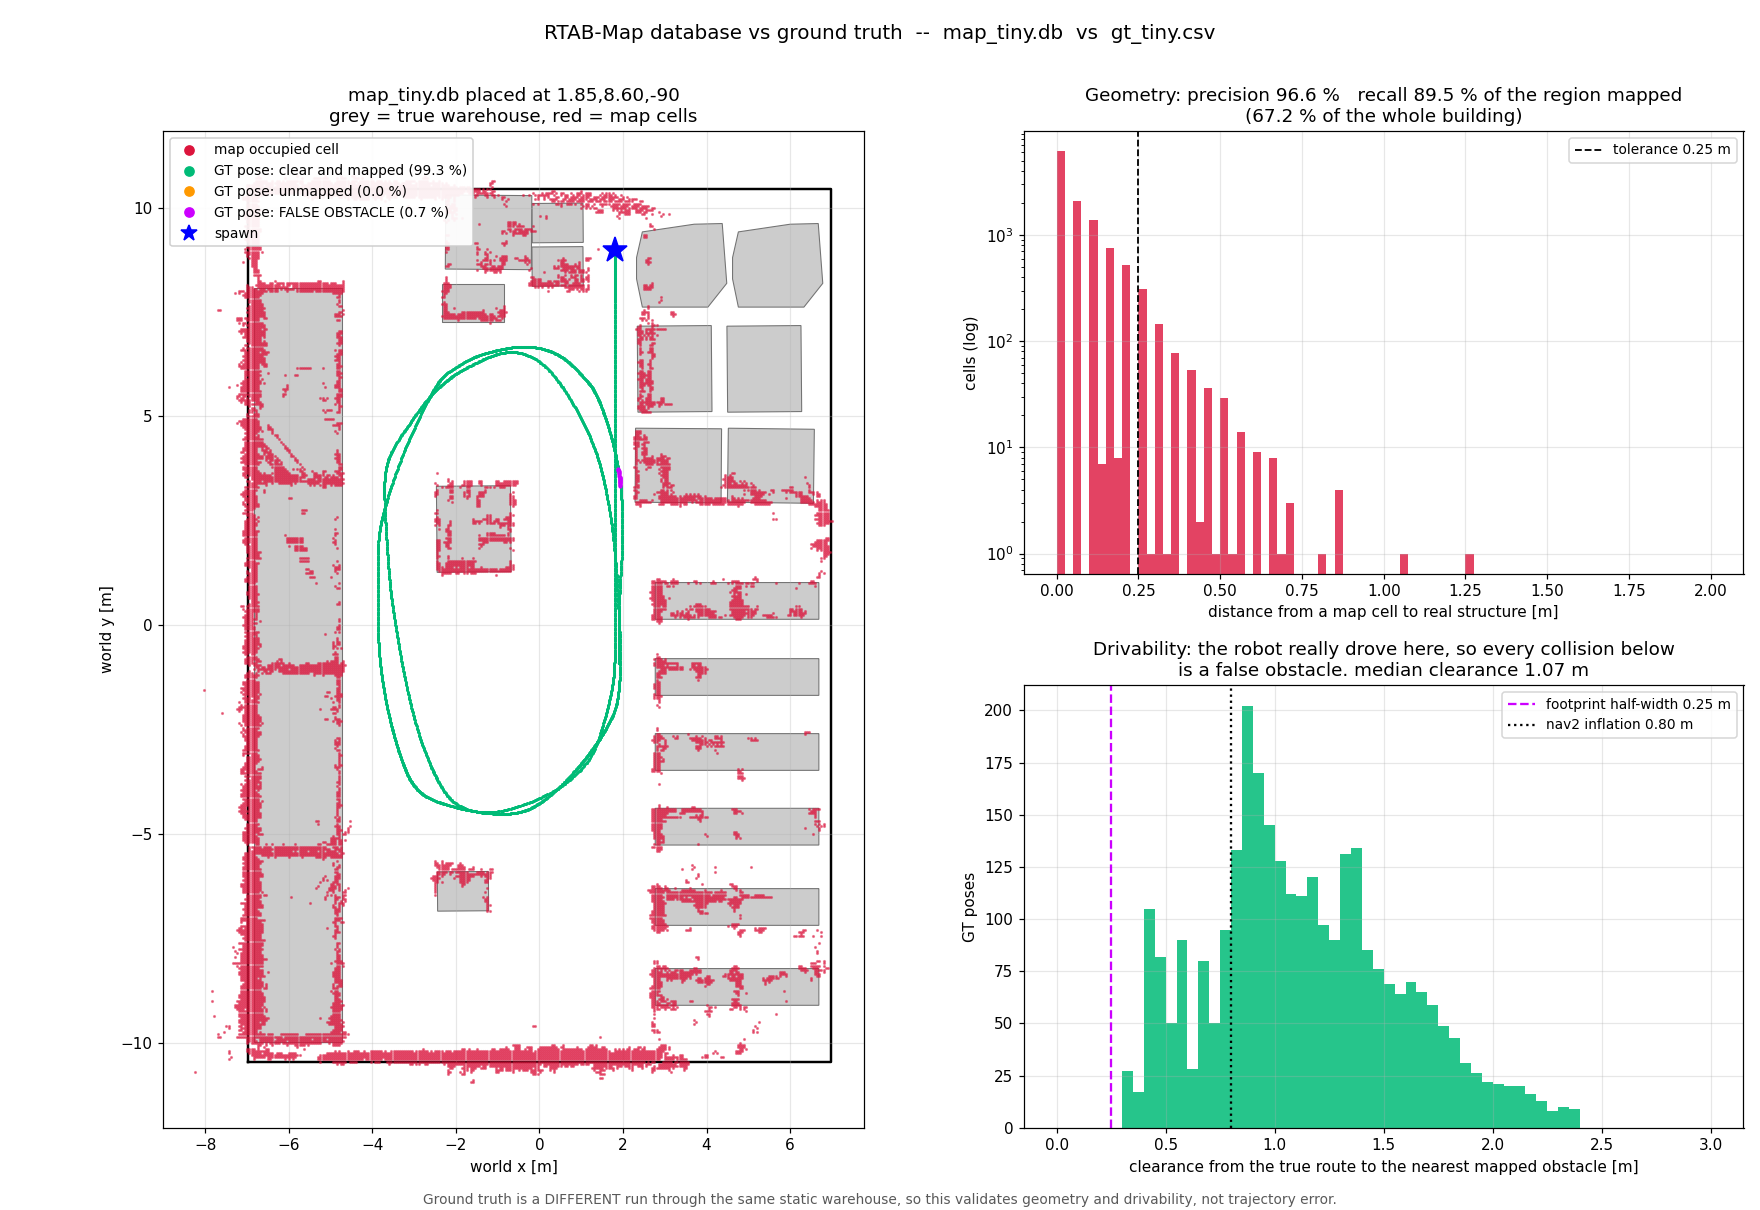
\includegraphics[width=\textwidth]{../../../output/compare/rtab_map_vs_gt.png}
  \caption{Dense-map evaluation of \repo{map/map_tiny.db}. Left: occupied cells
  (red) over the world file's true collision geometry (grey), with the
  ground-truth route coloured by drivability and the spawn marked. Top right:
  distance from each occupied cell to real structure, with the
  \SI{0.25}{\metre} tolerance marked; the bulk falls well inside tolerance with a
  thin tail to about \SI{1.25}{\metre}. Bottom right: clearance from the true
  route to the nearest mapped obstacle, against the footprint half-width and the
  nav2 inflation radius. The ground truth was a different run through the same
  static warehouse, so this validates geometry and drivability, not trajectory
  error; that run is no longer available
  (\cref{sec:map-drivability}).}
  \label{fig:map-vs-gt}
\end{figure}

\begin{figure}[htbp]
  \centering
  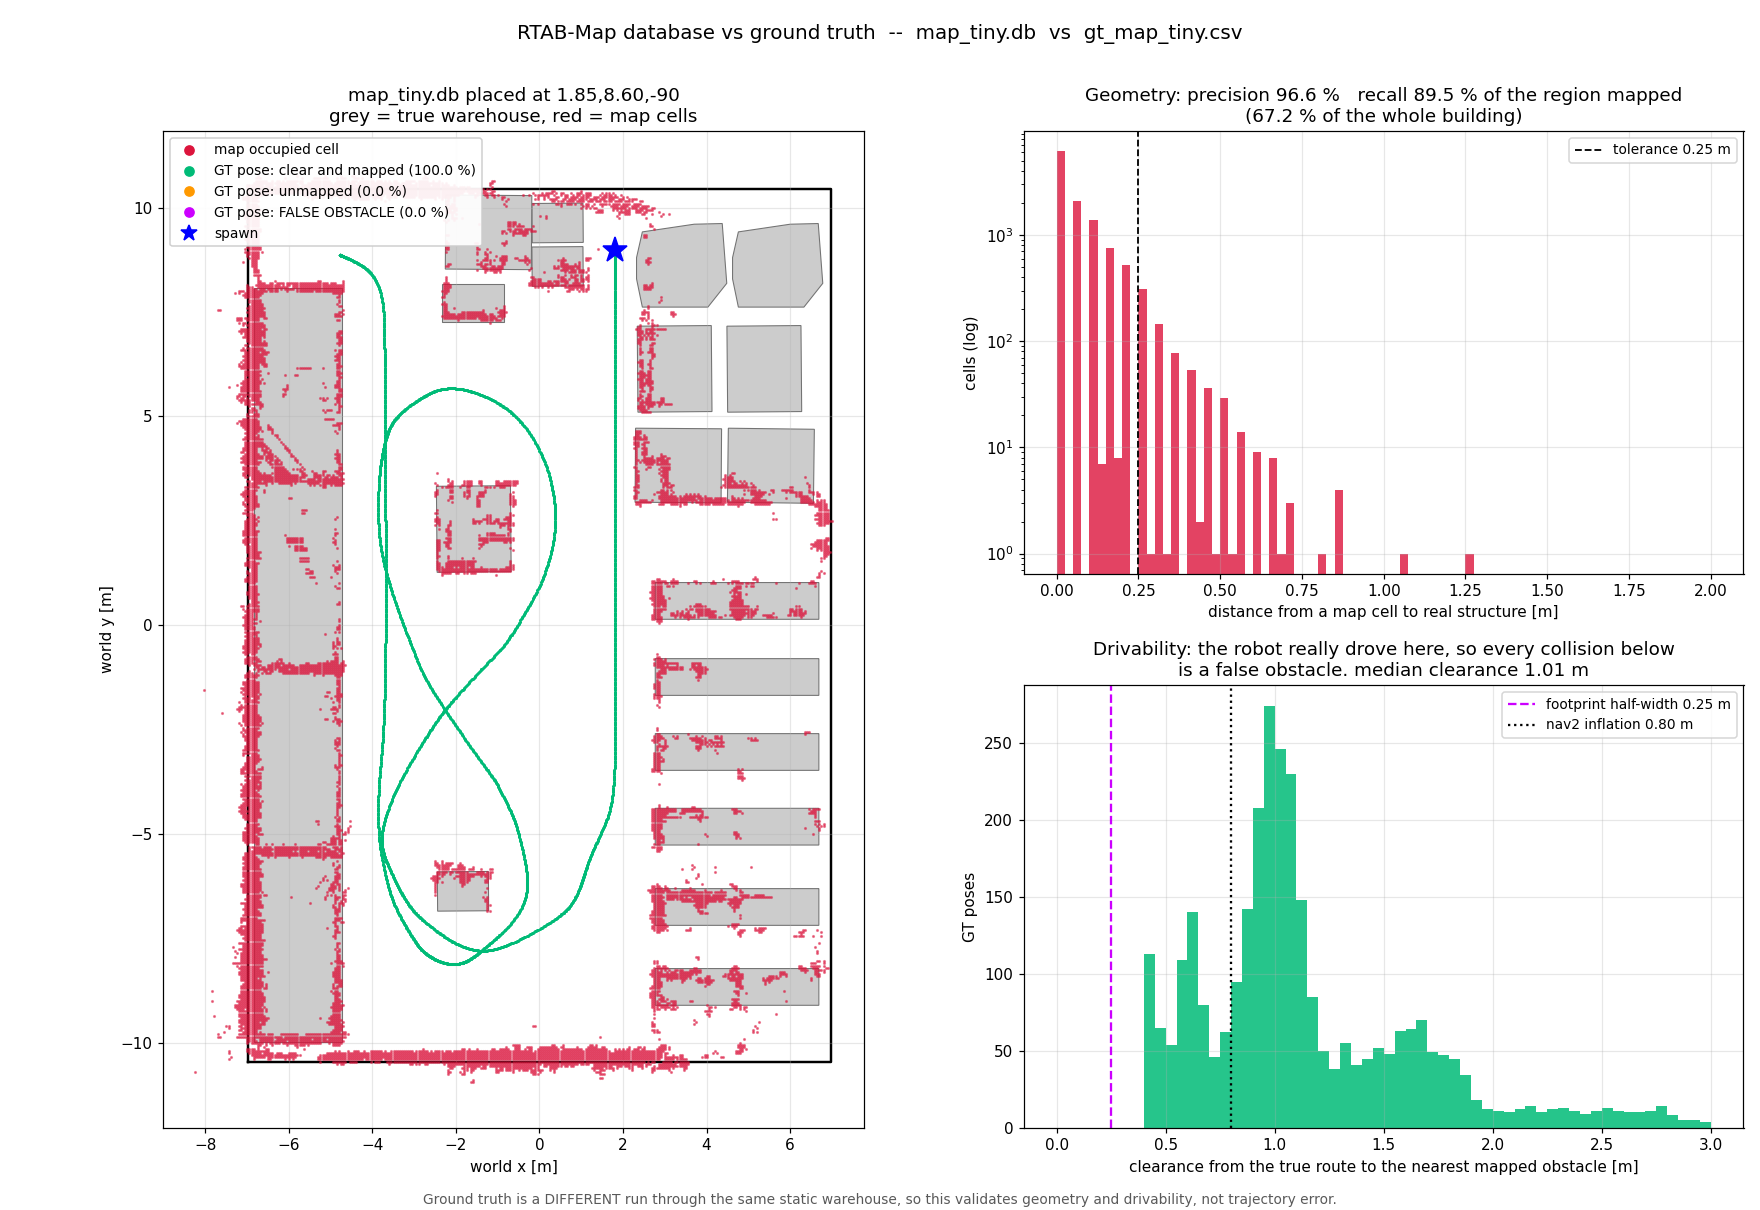
\includegraphics[width=\textwidth]{../../../output/compare/rtab_map_vs_gt_selfcheck.png}
  \caption{The same database scored against the run that built it,
  \repo{dataset/dataset_map_tiny}. The route is a figure-eight rather than the
  oval of \cref{fig:map-vs-gt}, and no pose on it collides with the map: the
  false-obstacle rate falls from \SI{0.7}{\percent} to \SI{0.0}{\percent}. The
  geometry panels are identical to \cref{fig:map-vs-gt} because geometry does not
  depend on the route. The footer claiming a different run is emitted
  unconditionally by the evaluator and is incorrect for this figure.}
  \label{fig:map-vs-gt-selfcheck}
\end{figure}

\subsection{Interpretation and limitations}

Within its stated scope the tiny map is geometrically faithful and navigable:
\SI{96.6}{\percent} of what it marks as occupied is real, it recovers
\SI{89.5}{\percent} of the surfaces it actually observed, and it contains no blind
cells and only \SI{0.7}{\percent} proven false obstacles along a route the robot
really drove. The geometry half of that is independent evidence and is the
strongest map result the project currently holds; the drivability half is a
self-consistency check and is weaker than it looks. Both are a direct improvement
on earlier assessments that judged the same database unnavigable --- those were measured with the grid mis-seated, so the comparison
was against the wrong cells. That correction is a methodological finding in its
own right and is why \cref{sec:map-quality} reports placement before any metric.

Four limitations bound what these numbers support.

\begin{itemize}
  \item \textbf{The drivability reference cannot be re-read.} The run that
    provided it is lost, and the only surviving recording of this warehouse is the
    one that built the map, which would answer a weaker question. Re-establishing
    this result needs a fresh independent recording --- a second run, not a second
    map.
  \item \textbf{The route is easy.} It is one large loop down the wide central
    aisle and never squeezes into a side aisle. The \SI{0.7}{\percent} false-obstacle
    figure is therefore a floor, not a worst case. A route through the narrow
    aisles is the test that would actually stress this map, and it has not been
    run.
  \item \textbf{Clearance couples to planner cost.} The 5th-percentile clearance
    of \SI{0.45}{\metre} sits below nav2's \SI{0.80}{\metre} inflation radius, and
    a visible share of the true route lies inside it. Nothing is blocked, but a
    planner would charge a high cost for driving where the robot demonstrably
    drove. That coupling should be examined before any planned path is trusted.
  \item \textbf{$n=1$, and the scope is one world.} A single database on the tiny
    warehouse supports no uncertainty estimate and no claim about the large
    warehouse, where longer routes and narrower bays change both the drift
    exposure and the clearance margin.
  \item \textbf{Residual distortion is not a placement problem.} Walls appear
    doubled and thickened and shelf rows bowed in the overlay. No rigid transform
    removes that; it is internal map distortion and is the property that would
    limit navigation, independently of how well the grid is seated.
\end{itemize}

\begin{queried}[Queried: reproducibility of the drivability half]
The geometry result is fully reproducible: both \repo{map/map_tiny.db} and the
world file are present. The drivability result is not. Its reference run,
\repo{dataset_static_tiny_repeat}, is absent from \repo{dataset/} and from the
removable drive, and the only surviving recording of this warehouse is the one
that built the map, which would answer a weaker question
(\cref{sec:map-drivability}). The database additionally stores an empty parameter
set, so the configuration that produced it is not recoverable from the file, and
the RTAB-Map engineering record's claim that the node stamps match no dataset is
contradicted by the pose agreement reported above. The drivability figures should
therefore be read as a dated measurement rather than a standing result, and should
not be carried into the major report until an independent route has been recorded
and retained.
\end{queried}

\subsection{Planned extension to the large warehouse}

The same evaluation is \status{planned} for the large warehouse and is not
started: no large-map database exists at the cutoff. Three things must be settled
before those numbers would mean anything. The world-to-map placement must be
measured for the new database rather than assumed, since the tiny-map constant
$(1.850, 8.600, \SI{-89.90}{\degree})$ is specific to that database and world. A
ground-truth route must be recorded from a run \emph{other} than the one that
builds the map, which the tiny-map case did not do and which is what would turn
drivability into independent evidence. Finally, the route should deliberately
include narrow bays, so that the false-obstacle rate is exercised rather than
merely reported. Until then,
no map-quality claim extends beyond the tiny warehouse.

\section{Loop Closure, Map Merging, and Global-Correction Evidence}
\label{sec:global-events}

The expanded ORB logs now expose back-end events. Baseline ORB-SLAM3 recorded six
loop closures: two in each repeat of
\repo{dataset_static_nofloortexture_002}. Each of those runs also recorded two
global bundle-adjustment executions. One baseline dynamic run
(\repo{dataset_dynamic_nofloortexture_02_000/logging_20260916_03}) and one
ORB+YOLO run
(\repo{dataset_dynamic_nofloortexture_01_000/logging_20260916_02}) recorded a map
merge. These counters demonstrate that the native ORB back-end paths executed;
they do not demonstrate that the resulting corrections were correct. The
failed trajectory-plausibility checks and the absence of an event-aligned
before/after counterfactual prevent a correction-benefit claim. RTAB-Map reconstruction remains a separate pipeline and is not exercised by
this relogged campaign; its dense-map evidence is reported independently in
\cref{sec:map-quality}, on a different world and database.

\section{Interpretation, Limitations, and Advisor Decisions}
\label{sec:results-discussion}


\subsection{Where each pipeline is weak, block by block}
\label{sec:block-performance}

\Cref{fig:blockperf-static,fig:blockperf-dynamic} put every instrumented stage of
the three pipelines on one page and colour it by a stated criterion.
\Cref{tab:blockperf-static-orb} through \cref{tab:blockperf-dynamic-vins} give the evidence behind every
colour: the metric, its value, the criterion it was tested against, and which of
three rules produced the verdict. Both the figures' fills and the tables are
generated by \repo{script/block_performance.py} from the run artifacts; no colour
in either figure was chosen by hand.

The three rules are deliberately distinguished, because they answer different
questions and only one of them is about accuracy:

\begin{description}[leftmargin=2.2em,style=nextline]
  \item[ablation] The block was removed, disabled or swapped and the run repeated.
    The value is the ratio of aligned ATE without it to aligned ATE with it. This
    is the only rule that speaks to trajectory error.
  \item[latency] The block's median time as a share of its stage, or a stage
    against the \SI{66.0}{\milli\second} inter-frame budget implied by
    \SI{30.3}{\hertz} imagery at $0.5\times$ replay. Describes cost, not accuracy.
  \item[outcome] A counter the block emits, against a stated threshold---accepted
    loop candidates, usable solver solutions, filter consistency.
\end{description}

\paragraph{Where the criteria come from.}
Every verdict is a comparison against a threshold, and those thresholds do not all
have the same standing. The tables label each one, and the distinction matters
more than the values:

\begin{description}[leftmargin=2.4em,style=nextline]
  \item[\textit{derived}] Follows from something outside this report. There are
    two. The \SI{66.0}{\milli\second} frame budget is arithmetic on the recorded
    conditions, $1000/(30.3\,\mathrm{Hz}\times0.5$ replay$)$: a per-frame stage
    slower than this cannot keep up, and no judgement is involved. The consistency
    target $\mathrm{ANEES}=3.0$ is the standard result that a correctly scaled
    covariance makes the normalised error squared average the degrees of freedom,
    which for a pose error is three.
  \item[\textit{convention}] A round number adopted here so the rule is stated
    rather than left implicit. Nothing external fixes \SI{40}{\percent} of a stage
    rather than \SI{35}{\percent}, $2.0\times$ for a load-bearing block rather than
    $1.5\times$, \SI{10}{\percent} of loop candidates accepted, or
    \SI{99}{\percent} of solver calls returning a usable solution. These are
    contestable, which is why the measured value sits beside the threshold in
    every row: a reader who prefers a different line can redraw it without
    re-running anything.
\end{description}

\begin{queried}[Withdrawn criterion]
An earlier revision of these tables graded VINS-Fusion's solver quality against
``median final cost $>5000$''. That threshold was chosen after observing 1176 in
static scenes and 14110 in dynamic ones, so it separated two numbers already in
hand and the \flag{``poor'' verdict it produced was guaranteed by the choice
rather than tested by it}. Raw Ceres cost also has no absolute scale, depending on
residual count and weighting, so no fixed threshold on it is meaningful in
principle. It is replaced by the solver's own \repo{solver_solution_usable} flag,
which is binary and emitted by the solver rather than invented here:
\SI{99.64}{\percent} of solves in static scenes and \SI{99.55}{\percent} in
dynamic ones return a usable solution, and the block is now graded \perfmark{good}
in both. The non-convergence rate---\SI{22.9}{\percent} of solves in static scenes
and \SI{45.3}{\percent} in dynamic ones reaching the iteration or
\SI{80}{\milli\second} cap---is reported in the note column and deliberately not
graded, because any threshold on it would repeat the same error.
\end{queried}

\begin{queried}[Reading the colours]
A red block is \emph{not} a claim that it caused the trajectory error, unless its
rule is \texttt{ablation}. Only four blocks in the entire project have an
ablation behind them: the EKF's wheel correction, its IMU prediction, its
yaw-rate model, and ORB-SLAM3's loop closing. Every other red marks a block that
is expensive or that emits a poor counter, which is a different and weaker
statement. Yellow means no claim at all---not instrumented, not exercised in these
runs, or not implemented in this fork.
\end{queried}

\begin{figure}[p]
  \centering
  %% Generated by script/block_performance.py -- do not edit.
\expandafter\def\csname blockcolour@static@orbextract\endcsname{perfpoor}
\expandafter\def\csname blockcolour@static@orbimupre\endcsname{perfgood}
\expandafter\def\csname blockcolour@static@orbposepred\endcsname{perfgood}
\expandafter\def\csname blockcolour@static@orbtracklocal\endcsname{perfgood}
\expandafter\def\csname blockcolour@static@orbkfdec\endcsname{perfgood}
\expandafter\def\csname blockcolour@static@orbkfins\endcsname{perfgood}
\expandafter\def\csname blockcolour@static@orbmpcull\endcsname{perfgood}
\expandafter\def\csname blockcolour@static@orbnewpoints\endcsname{perfgood}
\expandafter\def\csname blockcolour@static@orblba\endcsname{perfpoor}
\expandafter\def\csname blockcolour@static@orbkfcull\endcsname{perfgood}
\expandafter\def\csname blockcolour@static@orbtrackingtotal\endcsname{perfgood}
\expandafter\def\csname blockcolour@static@orbimuinit\endcsname{perfgood}
\expandafter\def\csname blockcolour@static@orbimuref\endcsname{perfgood}
\expandafter\def\csname blockcolour@static@orbplacerec\endcsname{perfpoor}
\expandafter\def\csname blockcolour@static@orbloopfusion\endcsname{perfpoor}
\expandafter\def\csname blockcolour@static@orbfullba\endcsname{perfnone}
\expandafter\def\csname blockcolour@static@orbyolo\endcsname{perfnone}
\expandafter\def\csname blockcolour@static@vinstrack\endcsname{perfgood}
\expandafter\def\csname blockcolour@static@vinsqueue\endcsname{perfpoor}
\expandafter\def\csname blockcolour@static@vinsimuprop\endcsname{perfgood}
\expandafter\def\csname blockcolour@static@vinstri\endcsname{perfgood}
\expandafter\def\csname blockcolour@static@vinsconstruct\endcsname{perfgood}
\expandafter\def\csname blockcolour@static@vinssolve\endcsname{perfpoor}
\expandafter\def\csname blockcolour@static@vinsmarg\endcsname{perfgood}
\expandafter\def\csname blockcolour@static@vinsoutlier\endcsname{perfgood}
\expandafter\def\csname blockcolour@static@vinsslide\endcsname{perfgood}
\expandafter\def\csname blockcolour@static@vinsbackendtotal\endcsname{perfpoor}
\expandafter\def\csname blockcolour@static@vinssolverq\endcsname{perfgood}
\expandafter\def\csname blockcolour@static@vinsloop\endcsname{perfnone}
\expandafter\def\csname blockcolour@static@vinsrtab\endcsname{perfnone}
\expandafter\def\csname blockcolour@static@vinsyolo\endcsname{perfnone}
\expandafter\def\csname blockcolour@static@ekfwheelupd\endcsname{perfgood}
\expandafter\def\csname blockcolour@static@ekfbiasobs\endcsname{perfgood}
\expandafter\def\csname blockcolour@static@ekfimupred\endcsname{perfgood}
\expandafter\def\csname blockcolour@static@ekfyaw\endcsname{perfpoor}
\expandafter\def\csname blockcolour@static@ekfanchor\endcsname{perfnone}
\expandafter\def\csname blockcolour@static@ekfcov\endcsname{perfpoor}
%
  \resizebox{\textwidth}{!}{\pipelinefig{static}}
  \caption{Per-block performance in the \textbf{static} condition, over the five
  \repo{allsensor} datasets. The EKF baseline appears here and not in
  \cref{fig:blockperf-dynamic} because no dynamic dataset carries wheel encoders.
  Evidence for every colour is in \cref{tab:blockperf-static-orb,tab:blockperf-static-vins,tab:blockperf-static-ekf}, one table per algorithm.}
  \label{fig:blockperf-static}
\end{figure}
\clearpage

\begin{table}[p]
\centering
\caption{Per-block evidence for \textbf{ORB-SLAM3} in the static condition, \cref{fig:blockperf-static}. Five \repo{allsensor} datasets, median across runs, loop closing enabled (\repo{logging_20260916_01}).}
\label{tab:blockperf-static-orb}
\scriptsize
\setlength{\tabcolsep}{3pt}
%% Generated by script/block_performance.py -- do not edit.
\begin{tabularx}{\textwidth}{>{\raggedright\arraybackslash}p{0.155\textwidth}l>{\raggedright\arraybackslash}X r>{\raggedright\arraybackslash}p{0.20\textwidth}l}
\toprule
Block & Rule & Metric & Value & Criterion / note & Verdict \\
\midrule
\multicolumn{6}{l}{\textbf{Tracking}} \\
\addlinespace[2pt]
\quad Extract ORB (+preproc, stereo) & latency & median image\_preprocessing\_feature\_stereo\_ms & \num{33.1} & \textit{convention:} $<$40\% of stage (61.4\% of stage) & \perfmark{poor} \\
\addlinespace[3.5pt]
\quad IMU preintegration & latency & median imu\_preintegration\_ms & \num{0.120} & \textit{convention:} $<$40\% of stage (0.2\% of stage) & \perfmark{good} \\
\addlinespace[3.5pt]
\quad Initial pose estimation & latency & median pose\_prediction\_ms & \num{0.087} & \textit{convention:} $<$40\% of stage (0.2\% of stage) & \perfmark{good} \\
\addlinespace[3.5pt]
\quad Track local map & latency & median local\_map\_tracking\_ms & \num{16.5} & \textit{convention:} $<$40\% of stage (30.7\% of stage) & \perfmark{good} \\
\addlinespace[3.5pt]
\quad New keyframe decision & latency & median keyframe\_decision\_ms & \num{0.169} & \textit{convention:} $<$40\% of stage (0.3\% of stage) & \perfmark{good} \\
\addlinespace[3.5pt]
\quad TRACKING total & latency & median tracking\_total\_ms & \num{53.8} & \textit{derived:} $<$\SI{66.0}{\milli\second} frame budget & \perfmark{good} \\
\addlinespace[3.5pt]
\quad Dynamic feature removal (YOLO) & none & -- & -- & -- (filter disabled in every run reported here) & \perfmark{none} \\
\addlinespace[3.5pt]
\addlinespace[5pt]
\multicolumn{6}{l}{\textbf{Local mapping}} \\
\addlinespace[2pt]
\quad KeyFrame insertion & latency & median keyframe\_insertion\_ms & \num{10.3} & \textit{convention:} $<$40\% of stage (3.3\% of stage) & \perfmark{good} \\
\addlinespace[3.5pt]
\quad Recent MapPoints culling & latency & median map\_point\_culling\_ms & \num{0.383} & \textit{convention:} $<$40\% of stage (0.1\% of stage) & \perfmark{good} \\
\addlinespace[3.5pt]
\quad New points creation & latency & median map\_point\_creation\_fusion\_ms & \num{41.5} & \textit{convention:} $<$40\% of stage (13.3\% of stage) & \perfmark{good} \\
\addlinespace[3.5pt]
\quad Local BA & latency & median local\_ba\_ms & \num{244.4} & \textit{convention:} $<$40\% of stage (78.1\% of stage) & \perfmark{poor} \\
\addlinespace[3.5pt]
\quad Local keyframes culling & latency & median keyframe\_culling\_ms & \num{10.9} & \textit{convention:} $<$40\% of stage (3.5\% of stage) & \perfmark{good} \\
\addlinespace[3.5pt]
\quad IMU initialization & latency & median imu\_initialization\_ms & \num{0.002} & \textit{convention:} $<$40\% of stage (negligible) & \perfmark{good} \\
\addlinespace[3.5pt]
\quad IMU scale refinement & latency & median inertial\_refinement\_ms & \num{0.001} & \textit{convention:} $<$40\% of stage (negligible) & \perfmark{good} \\
\addlinespace[3.5pt]
\addlinespace[5pt]
\multicolumn{6}{l}{\textbf{Loop closing}} \\
\addlinespace[2pt]
\quad Place recognition & outcome & candidates accepted & 4 of 281 & \textit{convention:} $>$\SI{10}{\percent} of candidates accepted (2494 events) & \perfmark{poor} \\
\addlinespace[3.5pt]
\quad Loop fusion + essential graph & ablation & ATE(on)/ATE(off) & 1.37 & \textit{convention:} $<$1.0 (enabling it should help) (one run per configuration) & \perfmark{poor} \\
\addlinespace[3.5pt]
\quad Full BA & outcome & global BA executions & -- & -- (see \cref{tab:orb-loop}) & \perfmark{none} \\
\addlinespace[3.5pt]
\bottomrule
\end{tabularx}

\end{table}
\clearpage
\begin{table}[p]
\centering
\caption{Per-block evidence for \textbf{VINS-Fusion} in the static condition, \cref{fig:blockperf-static}. Five \repo{allsensor} datasets, median across runs.}
\label{tab:blockperf-static-vins}
\scriptsize
\setlength{\tabcolsep}{3pt}
%% Generated by script/block_performance.py -- do not edit.
\begin{tabularx}{\textwidth}{>{\raggedright\arraybackslash}p{0.155\textwidth}l>{\raggedright\arraybackslash}X r>{\raggedright\arraybackslash}p{0.20\textwidth}l}
\toprule
Block & Rule & Metric & Value & Criterion / note & Verdict \\
\midrule
\multicolumn{6}{l}{\textbf{Front end}} \\
\addlinespace[2pt]
\quad Feature tracking & latency & median feature\_tracking\_ms & \num{55.2} & $<$\SI{66.0}{\milli\second} frame budget & \perfmark{good} \\
\addlinespace[3.5pt]
\quad Feature queue & latency & median feature\_queue\_wait\_ms & \num{403.7} & $<$\SI{66.0}{\milli\second} frame budget (backlog 4.0 frames) & \perfmark{poor} \\
\addlinespace[3.5pt]
\quad Persistent-feature removal (YOLO) & none & -- & -- & -- (filter disabled in every run reported here) & \perfmark{none} \\
\addlinespace[3.5pt]
\addlinespace[5pt]
\multicolumn{6}{l}{\textbf{Back end}} \\
\addlinespace[2pt]
\quad IMU propagation & latency & median imu\_propagation\_ms & \num{0.272} & \textit{convention:} $<$40\% of stage (0.4\% of stage) & \perfmark{good} \\
\addlinespace[3.5pt]
\quad Triangulation & latency & median triangulation\_ms & \num{0.063} & \textit{convention:} $<$40\% of stage (0.1\% of stage) & \perfmark{good} \\
\addlinespace[3.5pt]
\quad Problem construction & latency & median problem\_construction\_ms & \num{3.2} & \textit{convention:} $<$40\% of stage (4.7\% of stage) & \perfmark{good} \\
\addlinespace[3.5pt]
\quad Ceres solve & latency & median solver\_ms & \num{48.3} & \textit{convention:} $<$40\% of stage (71.9\% of stage) & \perfmark{poor} \\
\addlinespace[3.5pt]
\quad Marginalization & latency & median marginalization\_ms & \num{4.1} & \textit{convention:} $<$40\% of stage (6.1\% of stage) & \perfmark{good} \\
\addlinespace[3.5pt]
\quad Outlier rejection & latency & median outlier\_rejection\_ms & \num{0.155} & \textit{convention:} $<$40\% of stage (0.2\% of stage) & \perfmark{good} \\
\addlinespace[3.5pt]
\quad Slide window & latency & median slide\_window\_ms & \num{0.212} & \textit{convention:} $<$40\% of stage (0.3\% of stage) & \perfmark{good} \\
\addlinespace[3.5pt]
\quad BACK END total & latency & median backend\_total\_ms & \num{67.2} & $<$\SI{66.0}{\milli\second} frame budget & \perfmark{poor} \\
\addlinespace[3.5pt]
\quad Solver convergence & outcome & solves returning a usable solution & 99.64\% & \textit{convention:} $\geq$\SI{99}{\percent} usable (\SI{22.8}{\percent} hit the iteration or \SI{80}{\milli\second} cap without converging; reported, not graded) & \perfmark{good} \\
\addlinespace[3.5pt]
\addlinespace[5pt]
\multicolumn{6}{l}{\textbf{Loop closing}} \\
\addlinespace[2pt]
\quad Loop fusion & none & -- & -- & -- (not implemented in this fork) & \perfmark{none} \\
\addlinespace[3.5pt]
\quad RTAB-Map correction & none & -- & -- & -- (separate process; correction never injected) & \perfmark{none} \\
\addlinespace[3.5pt]
\bottomrule
\end{tabularx}

\end{table}
\clearpage
\begin{table}[p]
\centering
\caption{Per-block evidence for the \textbf{EKF wheel\,+\,IMU} baseline, \cref{fig:blockperf-static}. Every row but the last two is an ablation: the block was removed or swapped and all five datasets re-run, so these are the only verdicts in this section that speak to trajectory error.}
\label{tab:blockperf-static-ekf}
\scriptsize
\setlength{\tabcolsep}{3pt}
%% Generated by script/block_performance.py -- do not edit.
\begin{tabularx}{\textwidth}{>{\raggedright\arraybackslash}p{0.155\textwidth}l>{\raggedright\arraybackslash}X r>{\raggedright\arraybackslash}p{0.20\textwidth}l}
\toprule
Block & Rule & Metric & Value & Criterion / note & Verdict \\
\midrule
\multicolumn{6}{l}{\textbf{EKF}} \\
\addlinespace[2pt]
\quad Wheel speed correction & ablation & ATE without the wheel update / with & 54.08 & \textit{convention:} $\geq$2.0$\times$ (block is load-bearing) (median over 5 bags; joint with the other row -- one flag removes both) & \perfmark{good} \\
\addlinespace[3.5pt]
\quad Gyro-bias observation & ablation & ATE without the wheel update / with & 54.08 & \textit{convention:} $\geq$2.0$\times$ (block is load-bearing) (median over 5 bags; joint with the other row -- one flag removes both) & \perfmark{good} \\
\addlinespace[3.5pt]
\quad IMU prediction & ablation & ATE of wheel-only / EKF & 6.56 & \textit{convention:} $\geq$2.0$\times$ (block is load-bearing) (median over 5 bags) & \perfmark{good} \\
\addlinespace[3.5pt]
\quad Yaw-rate model (bicycle) & ablation & ATE with differential / with bicycle & 1.02 & \textit{convention:} $\geq$2.0$\times$ (block is load-bearing) (median over 5 bags) & \perfmark{poor} \\
\addlinespace[3.5pt]
\quad Initial pose anchor & none & -- & -- & -- (ground-truth pose; not a performance block) & \perfmark{none} \\
\addlinespace[3.5pt]
\quad Covariance propagation & outcome & ANEES (3 DOF) & -- & \textit{derived:} 3.0 for a consistent filter (64.7--123.2; see \cref{tab:proprio-covariance}) & \perfmark{poor} \\
\addlinespace[3.5pt]
\bottomrule
\end{tabularx}

\end{table}
\clearpage
\begin{figure}[p]
  \centering
  %% Generated by script/block_performance.py -- do not edit.
\expandafter\def\csname blockcolour@dynamic@orbextract\endcsname{perfpoor}
\expandafter\def\csname blockcolour@dynamic@orbimupre\endcsname{perfgood}
\expandafter\def\csname blockcolour@dynamic@orbposepred\endcsname{perfgood}
\expandafter\def\csname blockcolour@dynamic@orbtracklocal\endcsname{perfgood}
\expandafter\def\csname blockcolour@dynamic@orbkfdec\endcsname{perfgood}
\expandafter\def\csname blockcolour@dynamic@orbkfins\endcsname{perfgood}
\expandafter\def\csname blockcolour@dynamic@orbmpcull\endcsname{perfgood}
\expandafter\def\csname blockcolour@dynamic@orbnewpoints\endcsname{perfgood}
\expandafter\def\csname blockcolour@dynamic@orblba\endcsname{perfpoor}
\expandafter\def\csname blockcolour@dynamic@orbkfcull\endcsname{perfgood}
\expandafter\def\csname blockcolour@dynamic@orbtrackingtotal\endcsname{perfgood}
\expandafter\def\csname blockcolour@dynamic@orbimuinit\endcsname{perfnone}
\expandafter\def\csname blockcolour@dynamic@orbimuref\endcsname{perfnone}
\expandafter\def\csname blockcolour@dynamic@orbplacerec\endcsname{perfpoor}
\expandafter\def\csname blockcolour@dynamic@orbloopfusion\endcsname{perfnone}
\expandafter\def\csname blockcolour@dynamic@orbfullba\endcsname{perfnone}
\expandafter\def\csname blockcolour@dynamic@orbyolo\endcsname{perfnone}
\expandafter\def\csname blockcolour@dynamic@vinstrack\endcsname{perfgood}
\expandafter\def\csname blockcolour@dynamic@vinsqueue\endcsname{perfpoor}
\expandafter\def\csname blockcolour@dynamic@vinsimuprop\endcsname{perfgood}
\expandafter\def\csname blockcolour@dynamic@vinstri\endcsname{perfgood}
\expandafter\def\csname blockcolour@dynamic@vinsconstruct\endcsname{perfgood}
\expandafter\def\csname blockcolour@dynamic@vinssolve\endcsname{perfpoor}
\expandafter\def\csname blockcolour@dynamic@vinsmarg\endcsname{perfgood}
\expandafter\def\csname blockcolour@dynamic@vinsoutlier\endcsname{perfgood}
\expandafter\def\csname blockcolour@dynamic@vinsslide\endcsname{perfgood}
\expandafter\def\csname blockcolour@dynamic@vinsbackendtotal\endcsname{perfgood}
\expandafter\def\csname blockcolour@dynamic@vinssolverq\endcsname{perfgood}
\expandafter\def\csname blockcolour@dynamic@vinsloop\endcsname{perfnone}
\expandafter\def\csname blockcolour@dynamic@vinsrtab\endcsname{perfnone}
\expandafter\def\csname blockcolour@dynamic@vinsyolo\endcsname{perfnone}
%
  \resizebox{\textwidth}{!}{\pipelinefig{dynamic}}
  \caption{Per-block performance in the \textbf{dynamic} condition, over the
  twelve relogged dynamic runs of each estimator. Loop closing carries no
  ablation here because the relogged campaign has no loop-closure-disabled
  variant. Evidence in \cref{tab:blockperf-dynamic-orb,tab:blockperf-dynamic-vins},
  one table per algorithm.}
  \label{fig:blockperf-dynamic}
\end{figure}
\clearpage
\begin{table}[p]
\centering
\caption{Per-block evidence for \textbf{ORB-SLAM3} in the dynamic condition, \cref{fig:blockperf-dynamic}. Twelve relogged dynamic runs, median across runs.}
\label{tab:blockperf-dynamic-orb}
\scriptsize
\setlength{\tabcolsep}{3pt}
\input{tables/block_performance_dynamic_orb}
\end{table}
\clearpage
\begin{table}[p]
\centering
\caption{Per-block evidence for \textbf{VINS-Fusion} in the dynamic condition, \cref{fig:blockperf-dynamic}. Twelve relogged dynamic runs, median across runs.}
\label{tab:blockperf-dynamic-vins}
\scriptsize
\setlength{\tabcolsep}{3pt}
%% Generated by script/block_performance.py -- do not edit.
\begin{tabularx}{\textwidth}{>{\raggedright\arraybackslash}p{0.155\textwidth}l>{\raggedright\arraybackslash}X r>{\raggedright\arraybackslash}p{0.20\textwidth}l}
\toprule
Block & Rule & Metric & Value & Criterion / note & Verdict \\
\midrule
\multicolumn{6}{l}{\textbf{Front end}} \\
\addlinespace[2pt]
\quad Feature tracking & latency & median feature\_tracking\_ms & \num{42.5} & $<$\SI{66.0}{\milli\second} frame budget & \perfmark{good} \\
\addlinespace[3.5pt]
\quad Feature queue & latency & median feature\_queue\_wait\_ms & \num{502.1} & $<$\SI{66.0}{\milli\second} frame budget (backlog 7.5 frames) & \perfmark{poor} \\
\addlinespace[3.5pt]
\quad Persistent-feature removal (YOLO) & none & -- & -- & -- (filter disabled in every run reported here) & \perfmark{none} \\
\addlinespace[3.5pt]
\addlinespace[5pt]
\multicolumn{6}{l}{\textbf{Back end}} \\
\addlinespace[2pt]
\quad IMU propagation & latency & median imu\_propagation\_ms & \num{0.204} & \textit{convention:} $<$40\% of stage (0.3\% of stage) & \perfmark{good} \\
\addlinespace[3.5pt]
\quad Triangulation & latency & median triangulation\_ms & \num{0.062} & \textit{convention:} $<$40\% of stage (0.1\% of stage) & \perfmark{good} \\
\addlinespace[3.5pt]
\quad Problem construction & latency & median problem\_construction\_ms & \num{1.1} & \textit{convention:} $<$40\% of stage (1.7\% of stage) & \perfmark{good} \\
\addlinespace[3.5pt]
\quad Ceres solve & latency & median solver\_ms & \num{57.2} & \textit{convention:} $<$40\% of stage (89.8\% of stage) & \perfmark{poor} \\
\addlinespace[3.5pt]
\quad Marginalization & latency & median marginalization\_ms & \num{2.4} & \textit{convention:} $<$40\% of stage (3.7\% of stage) & \perfmark{good} \\
\addlinespace[3.5pt]
\quad Outlier rejection & latency & median outlier\_rejection\_ms & \num{0.068} & \textit{convention:} $<$40\% of stage (0.1\% of stage) & \perfmark{good} \\
\addlinespace[3.5pt]
\quad Slide window & latency & median slide\_window\_ms & \num{0.167} & \textit{convention:} $<$40\% of stage (0.3\% of stage) & \perfmark{good} \\
\addlinespace[3.5pt]
\quad BACK END total & latency & median backend\_total\_ms & \num{63.7} & $<$\SI{66.0}{\milli\second} frame budget & \perfmark{good} \\
\addlinespace[3.5pt]
\quad Solver convergence & outcome & solves returning a usable solution & 99.55\% & \textit{convention:} $\geq$\SI{99}{\percent} usable (\SI{45.1}{\percent} hit the iteration or \SI{80}{\milli\second} cap without converging; reported, not graded) & \perfmark{good} \\
\addlinespace[3.5pt]
\addlinespace[5pt]
\multicolumn{6}{l}{\textbf{Loop closing}} \\
\addlinespace[2pt]
\quad Loop fusion & none & -- & -- & -- (not implemented in this fork) & \perfmark{none} \\
\addlinespace[3.5pt]
\quad RTAB-Map correction & none & -- & -- & -- (separate process; correction never injected) & \perfmark{none} \\
\addlinespace[3.5pt]
\bottomrule
\end{tabularx}

\end{table}
\clearpage


Four readings follow that the trajectory tables alone do not give.

\textbf{Both visual front ends are the dominant cost, and neither keeps up
cleanly.} ORB-SLAM3 spends \SI{33.1}{\milli\second} of a \SI{53.8}{\milli\second}
tracking budget on preprocessing, extraction and stereo matching in static scenes,
rising to \SI{45.1}{\milli\second} of \SI{61.2}{\milli\second} in dynamic ones.
VINS-Fusion's back end waits \SI{403.7}{\milli\second} per frame on its feature
queue in static scenes and \SI{502.1}{\milli\second} in dynamic ones, against a
\SI{66.0}{\milli\second} frame budget, with a backlog of four to seven frames.
\flag{These are the same deficit wearing different clothes}: neither estimator
processes frames as fast as they arrive, and the two differ in what they do about
it. ORB-SLAM3 subscribes best-effort at depth five and discards the overflow,
which is the frame shortfall of \cref{sec:results-validity}; VINS-Fusion
subscribes reliably at depth 100 and absorbs it as latency. The frame counters see
one and not the other.

\textbf{Local BA dominates ORB-SLAM3's local mapping} at \SI{244.4}{\milli\second}
of \SI{312.9}{\milli\second} in static scenes. It runs per keyframe rather than
per frame, so it does not compete directly with the frame budget, but it is where
that pipeline's compute goes.

\textbf{Loop closing is not earning its place in these scenes.} Across the five
\repo{allsensor} datasets, enabling it leaves the median aligned ATE
\num{1.37} times \emph{worse} than disabling it, and only 4 of 281 place-recognition
candidates were ever accepted (\cref{tab:orb-loop}). This is the project's one
ORB-SLAM3 ablation, and it is still one run per configuration, so it sits inside
an unmeasured run-to-run spread---the verdict is reported, not relied upon.

\textbf{The EKF's accuracy rests on one intervention.} Removing the wheel update
costs a factor of \num{54} in aligned ATE; removing the IMU prediction costs
\num{6.6}. The \num{54} covers the wheel speed correction and the gyroscope-bias
observation \emph{together}: both are measurement rows of the same update, one
flag removes both, and no flag removes only one, so
\cref{tab:blockperf-static-ekf} lists the figure against each row while marking it
as joint rather than presenting two independent results. Swapping the yaw-rate model from the bicycle formulation to the
rear-wheel differential, by contrast, changes nothing measurable---median
\num{1.0}, and on \repo{allsensor_004} the noisier estimator is the better one.
That is worth stating plainly, because the differential model is four times worse
as a \emph{rate} estimator (\cref{tab:proprio-noise}) and dominates standalone
wheel odometry's error. Inside the filter it barely matters, because the wheel
rate is used only to observe the gyroscope bias and is weighted by its own
measured $\sigma$. The design choice of \cref{sec:proprio-method} is vindicated by
its own ablation.

The campaign succeeds as an instrumentation milestone: repeated run-level data,
front-end and back-end timing, input retention, process resources, initialization,
tracking loss, keyframes, loop closures, map merges, and raw trajectories are now
available in auditable form. Ground-truth accuracy can now be measured, but the
campaign does not support the intended semantic-filter hypothesis or a clean
dynamic-scene estimator ranking. The limitations are:

\Cref{tab:limitations} lists them with the consequence each one carries.

\begin{table}[htbp]
\centering
\caption{Limitations of the results reported in this chapter, and what each one
prevents. ``Scope'' identifies the experiment affected: R is the relogged
campaign, E the estimator comparison of \cref{sec:results-proprio}, and A both.}
\label{tab:limitations}
\small
\begin{tabularx}{\textwidth}{l>{\raggedright\arraybackslash}p{0.36\textwidth}>{\raggedright\arraybackslash}X}
\toprule
Scope & Limitation & Consequence \\
\midrule
A & RPE was missing & now implemented and reported (\cref{sec:rpe}); it
  withdrew this chapter's local-coherence reading \\
R & every dynamic trajectory fails the jump-plausibility criterion & no dynamic
  estimator ranking \\
R & the VINS semantic treatment was inactive in all repeats & no VINS filtering
  conclusion \\
R & 11 of 12 ORB treatment pairs fail the paired-input rule & no cross-treatment
  accuracy conclusion \\
R & YOLO truth is projected simulator geometry, not annotated visible extent, and
  the retained confidence threshold is fixed & no AP claim \\
R & class metrics are conditional on successful IoU localization & must not be
  read as end-to-end accuracy \\
R & two static ORB run summaries have incomplete schemas & retained as
  operational; counters unavailable \\
A & CPU and memory are per-estimator-process figures & not whole-system cost \\
A & one laptop and one replay rate throughout & no hardware or input-rate stress
  surface \\
E & \flag{replay rate $0.5\times$ for both visual estimators} & accuracy figures
  are not evidence of real-time capability \\
E & \flag{baselines are offline, visual estimators ran live} & timing-induced
  error is present on one side of the comparison only \\
E & \flag{only \repo{allsensor} bags carry wheel encoders} & the baseline exists
  for static featureless-floor scenes only; no dynamic condition \\
E & \flag{$n=5$ across four worlds, no condition repeated more than twice} & no
  mean, deviation or interval; between-bag differences are not effects \\
E & \flag{ORB-SLAM3 drops frames at a depth-5 best-effort subscriber; VINS buffers
  100 deep} & input delivery is not matched between the two; no timing comparison
  is admissible \\
E & \flag{ORB-SLAM3 run-to-run spread unmeasured, one run per configuration} &
  loop-closure differences cannot be attributed; repeats required \\
E & \flag{loop-closure state absent from \repo{run_metadata.csv}} & configurations
  distinguishable only by inspecting \repo{loop_closing.csv} \\
E & \flag{origin of the wheel yaw-rate offset untested} & the drift is predicted
  but not yet attributable or correctable (\cref{sec:h1-falsified}) \\
E & wheel-rate offset is absorbed by the EKF gyroscope-bias state & now
  quantified: EKF heading error rises tenfold where the wheel rate is poor
  (\cref{tab:ekf-coupling}) \\
E & \flag{accelerometer characterisation unstable across bags} & bias 0.019 to
  0.068, scale 1.020 to 1.067 for one simulated sensor \\
E & neither visual estimator writes a pose covariance & the consistency test
  cannot be applied to them \\
\bottomrule
\end{tabularx}
\end{table}

No root cause is assigned in this report. In particular, differences are not
attributed to calibration, timestamp handling, masks, replay scheduling, or a
specific estimator component without a controlled diagnostic experiment. The
immediate advisor decision is whether the next work period should first restore
active, input-matched filtering and plausible full trajectories, or
instead prioritize the planned integration of relocalization, global
optimization, and map merging. The latter remains future work and would provide
a unified localization/map input for navigation; path planning itself remains
outside scope.

\section*{Analysis Artifacts}
\addcontentsline{toc}{section}{Analysis Artifacts}

The numerical sources for this chapter are
\path{output/compare/relogged_20260916/run_metrics.csv},
\path{module_latency_summary.csv}, \path{trajectory_metrics.csv}, and
\path{pair_validity.csv}. The anomaly evidence is preserved in
\path{anomaly_catalog.csv} and \path{anomaly_run_metrics.csv}. The reproducible
offline renderers are \path{script/analyse_relogged_runs.py} and
\path{script/analyse_relogged_anomalies.py}. The per-run and example-run tables
in this chapter are typeset from \path{trajectory_metrics.csv} by
\path{script/make_result_tables.py}, which writes
\path{report/minor_report/tables/}; they are not hand-entered numbers.
Dense-map evidence is \path{map/map_tiny.db} with
\path{output/compare/rtab_map_vs_gt.png} (independent run) and
\path{rtab_map_vs_gt_selfcheck.png} (build run), produced by
\path{script/validate_map.py} with the placement measured by
\path{script/fit_map_pose.py}; the graph counts and the node-pose agreement were
read from the database read-only. Relative pose error is in
\path{rpe_metrics.csv} (interval sweep) with the \SI{1}{\second} values carried
into \path{trajectory_metrics.csv}; both tables are rendered by
\path{script/make_result_tables.py}. The evaluator prints its metrics to the console
and writes no machine-readable summary of its own, so both runs are transcribed to
\path{output/compare/rtab_map_vs_gt_metrics.csv}, with the second run's console
output preserved verbatim in \path{rtab_map_vs_gt_selfcheck.txt}. The first run's
console output was not captured and its ground-truth bag no longer exists, so its
row is transcribed from the engineering record. Offline detector evidence is stored
below \path{output/yolo_eval/dyn_00_000/}, \path{dyn_00_001/},
\path{dyn_01_000/}, and \path{dyn_02_000/}; the pooled source is
\path{summary_metrics.csv}, and the pooled detection association counts are in
\path{confusion_matrix.csv}. Conditional object-class results are in
\path{classification_confusion_matrix.csv} and
\path{classification_metrics.csv}. Its evaluator and summarizer are
\path{script/yolo_eval.py} and \path{script/summarise_yolo_eval.py}. Light and
dark figures, including one
comparison figure for every dataset/repeat group, are stored below
\path{output/compare/relogged_20260916/}; its \path{ground_truth/} subdirectory
contains the seven extracted rosbag truth trajectories. Raw estimator directories
and raw bags were not modified.
